% cd /home/gerald/van_development/van/aa
% cp /home/gerald/van_development/van/edu/latex/emoji.sty 
% 
% Build rules:
% pdflatex -shell-escape dia.tex
% evince dia.pdf

% This is the preamble of a LaTeX source code.
\documentclass[10pt,a4paper]{article}

% Import a package for a specific purpose: see https://www.ctan.org/
\usepackage[textwidth=17cm,textheight=26cm]{geometry}  % Customize the page layout.
\usepackage{tikzsymbols}    % Various emoticon, ...: \includegraphics.
\usepackage{enumitem}       % Control layout of itemize, enumerate, description.
\usepackage{wasysym}        % Provide symbols like \XBox.
\usepackage{scrextend}      % KOMA-Script class: labeling .
\usepackage{mdframed}       % Breakable framed and coloured boxes: mdframed.
\usepackage{anyfontsize}    % Select any font size: see \square.
\usepackage{stix}           % Complete set of mathematical glyphs: \boxtimes.
\usepackage[ngerman]{babel} % German orthography.
\usepackage{etoc}           % Table of contents control: \addcontentsline.
\usepackage{pdfpages}       % Inclusion of external PDF document: \includepdf.
\usepackage{colortbl}       % Allow rows and columns to be coloured: \rowcolor.
\usepackage{tcolorbox}      % Coloured and framed text boxes: tcolorbox
\tcbuselibrary{fitting,skins}
\usepackage{listings}       % Typeset programming code: lstlisting.
\usepackage{paracol}         % Multiple columns with texts in parallel: paracol.


% xxx
\usepackage{float}


% All paragraphs are without indentation.
\setlength{\parindent}{0pt}%


% Print a citiation left aligned.
\newcommand{\lmotto}[2]{%
  \begin{minipage}{0.33\textwidth}
    \small{} #1 \\
    \hspace*{\fill} #2
  \end{minipage}
  \topvskip\topvskip
}

% Print a citiation right aligned.
\newcommand{\rmotto}[2]{%
  \hfill
  \begin{minipage}{0.33\textwidth}
    \small{} #1 \\
    \hspace*{\fill} #2
  \end{minipage}
  \topvskip\topvskip
}

% Introduce a paragraph section with a number.
\renewcommand{\theparagraph}{\arabic{paragraph}.}

% Force the numbering of a paragraph text.
\setcounter{secnumdepth}{4}

% Settings for a sub paragraph segment.
% Increment the sub paragraph counter.
% Print the sub paragraph title.
% Extend the contents.
\newcommand\p[1] {%
  \stepcounter{paragraph}
  {\large\bf\theparagraph \hskip 2pt \large\bf #1 \ \hskip -8pt}
  \addcontentsline{toc}{section} {\theparagraph\hskip 3pt #1}
}

% Subparagraph counters.
\newcounter{subc}
\renewcommand{\thesubc}{\arabic{subc}.}

\newcounter{subsubc}
\renewcommand{\thesubsubc}{\arabic{subsubc}.}

% Settings for a sub paragraph segment.
% Increment the sub paragraph counter.
% Print the sub paragraph title.
% Extend the contents.
\newcommand\subp[1] {%
  \stepcounter{subc}
  {\bf\theparagraph\thesubc}\hskip 3pt\rm #1\hskip 4pt
  \addcontentsline{toc}{subsection}{\theparagraph\thesubc\hskip 3pt #1}
}

% Settings for a sub sub paragraph segment.
% Increment the sub sub paragraph counter.
% Print the sub sub paragraph title.
% Extend the contents.
\newcommand\subsubp[1] {%
  \stepcounter{subsubc}
  {\bf\theparagraph\thesubc\thesubsubc}\hskip 3pt\rm #1\hskip 4pt
  \addcontentsline{toc}{subsubsection}{\theparagraph\thesubc\thesubsubc\hskip 3pt #1}
}

% Note counter.
\newcounter{notec}
\newcommand\notep[1]{%
  \stepcounter{notec}
  \vskip #1pt
  {\bf\arabic{notec}.}
}

% Elements of a title page.
\newcommand\svthema{Diagnose}
\newcommand\svperson{Gerald Schüller}
\newcommand\svdatum{\today}


% Color list:
\definecolor{alizarin}{rgb}{0.82, 0.1, 0.26}
\definecolor{amber(sae/ece)}{rgb}{1.0, 0.49, 0.0}
\definecolor{amethyst}{rgb}{0.6, 0.4, 0.8}
\definecolor{aqua}{rgb}{0.0, 1.0, 1.0}
\definecolor{aquamarine}{rgb}{0.5, 1.0, 0.83}
\definecolor{battleshipgrey}{rgb}{0.52, 0.52, 0.51}  
\definecolor{burntorange}{rgb}{0.8, 0.33, 0.0}
% \definecolor{cornellred}{rgb}{0.7, 0.11, 0.11}  
\definecolor{darkbrown}{rgb}{0.4, 0.26, 0.13}
\definecolor{eggshell}{rgb}{0.94, 0.92, 0.84}
\definecolor{english}{rgb}{0.0, 0.5, 0.0}
\definecolor{indigo(web)}{rgb}{0.29, 0.0, 0.51}
\definecolor{midnightblue}{rgb}{0.1, 0.1, 0.44}


% Document and protocol track
\newcommand\expt[1] {{\color {darkbrown} {\bf #1}}}       % Experiment
\newcommand\info[1] {{\color {midnightblue} {\bf #1}}}    % Informatoin

\newcommand\prop[1] {{\color {alizarin} {\bf #1}}}        % Proposal
\newcommand\draf[1] {{\color {amber(sae/ece)} {\bf #1}}}  % Draft
\newcommand\rele[1] {{\color {english} \bf {#1}}}         % Release
\newcommand\rewo[1] {{\color {aqua} {\bf #1}}}            % Rework

\newcommand\emps[1] {{\color {indigo(web)} {\bf #1}}}     % Emphasis

\newcommand\opti[1] {{\color {amethyst} {\bf #1}}}        % Optional
\newcommand\mand[1] {{\color {burntorange} {\bf #1}}}     % Mandatory


% Frame list style of a single day.
\mdfdefinestyle{daystyle}{%
  skipabove=4pt,
  skipbelow=0pt,
  %  leftmargin=-16pt,
  leftmargin=-10pt,
  topline=false,
  bottomline=false,
  leftline=false,
  rightline=false
}

% Preceeding vertical skip of a paragramph.
\newcommand\topvskip {\vskip 8pt}

% Preceeding horizontal skip of a minipage.
\newcommand\tophskip {\hskip -14pt}

% Horizontal dividing line between two days.
\newcommand\ddivide {\vskip -9pt \hrule \vskip 6pt}

% First and last horizontal dividing line of a week.
\newcommand\fdivide {\vskip  6pt \hrule \vskip 6pt}
\newcommand\ldivide {\vskip -7pt \hrule \hrule \hrule \vskip 8pt}


% Top vertical space of a day list.
\newcommand\topspace{\vskip -15pt \hskip 20pt}

% Bottom vertical space of a day list.
\newcommand\bottomspace{\vskip 4pt}

% Set of natural numbers.
\newcommand{\N}{\mathbb{N}}

% Numbering of the day entries.
\newcommand\n[1] { {\sl #1.} \hskip 5pt }


% xxx
\usepackage{tabularx,ragged2e,booktabs}



% xxx
\usepackage[backend=biber,style=alphabetic,]{biblatex}

% biber dia
% pdflatex dia
% pdflatex dia
%
\addbibresource{books.bib}

\defbibheading{bibliography}[\bibname]{%
  \subsection{Bibliothek}%
  \markboth{#1}{#1}}

\defbibheading{subbibliography}[\bibname]{%
  \subsubsection{#1}%
  \markboth{#1}{#1}}



% Start of a LaTeX text, that is to be printed.
\begin{document}

% Front page
\title{ \textbf{\color{blue}\svthema} \Springtree [1.5] }
\author{ \textsl{\color{red}\svperson} --- \svdatum }
\date{}

% You tell LaTeX the information used to produce the title page.
\maketitle

% Multiple columns with texts in parallel.
\columnratio{0.5}
\begin{paracol}{2}
  % \lipsum[2]
  \lmotto{Meine Sätze erläutern $\ldots$, wenn er durch sie – auf ihnen – über
    sie hinausgestiegen ist. (Er muss sozusagen die Leiter wegwerfen, nachdem er
    auf ihr hinaufgestiegen ist.)}{L. Wittgenstein, Tractatus, {\bf 6.54}}
  
  \switchcolumn
  
  \rmotto{Der Fliege den Ausweg aus dem Fliegenglas zeigen.}{L. Wittgenstein, PU, 309.}
\end{paracol}

% \rmotto{Der Fliege den Ausweg aus dem Fliegenglas zeigen.}{L. Wittgenstein, PU, 309.}

% Generate the table of contents.
\tableofcontents

% Generate the apendix table.
\appendix

\newpage
\p{{\info {Track}}}

% Initialize the subparagraph counters.
\setcounter{subc}{0}

\topvskip
\begin{minipage}{0.90\textwidth} 
  \begin{labeling}{Information:} 
    \setlength\itemsep{-3pt}
  
  \item[Experiment:]  \textbackslash {\expt {expt}}
  \item[Information:] \textbackslash {\info {info}}
  \item[Proposal:]    \textbackslash {\prop {prop}}
  \item[Draft:]       \textbackslash {\draf {draf}}
  \item[Release:]     \textbackslash {\rele {rele}}
  \item[Rework:]      \textbackslash {\rewo {rewo}}
  \item[Emphasis:]    \textbackslash {\emps {emps}}
  \end{labeling}

\end{minipage}


\topvskip
\p{\info {Bibliographie}}

% Initialize the subparagraph counters.
\setcounter{subc}{0}

\topvskip
\verb+https://de.wikipedia.org/wiki/Diagnose+ \\
\verb+https:https://de.wikipedia.org/wiki/Befund_(Medizin)+ \\
\verb+https://de.wikipedia.org/wiki/Anamnese+ \\
\verb+https://de.wikipedia.org/wiki/%C3%84tiologie_(Medizin)+ \\
\verb+https://de.wikipedia.org/wiki/Pathogenese+ \\
\verb+https://de.wikipedia.org/wiki/Labordiagnostik+ \\
\verb+https://de.wikipedia.org/wiki/ICD-10+ \\
\verb+https://www.icd-code.de/suche/icd/recherche.html?sp=0&sp=SAlkoholkrankheit+

\topvskip
\verb+https://tex.stackexchange.com/questions/329228/+ \\
\verb+writing-texts-in-two-parallel-columns+ \\
\verb+https://people.umass.edu/klement/tlp/tlp.pdf+

\topvskip
\p{\info {Definitionen}}

% Initialize the subparagraph counters.
\setcounter{subc}{0}

\tophskip
\begin{minipage}{0.90\textwidth}  
  \begin{itemize}
    \setlength\itemsep{-3pt}

  \item {\emps {Befund}} bezeichnet den körperlichen und psychischen Zustand und
    Veränderungen, die vom Fachpersonal beschrieben werden.

  \item {\emps {Anamnese}} ist die Erfragung von medizinischen Informationen
    durch Fachpersonal mit dem Ziel, die Krankkengeschichte eines Patienten aufzuklären.
    
  \item {\emps {Diagnose}} ist die Bestimmung einer Krankheit durch die
    Zusammenfassung der ermittelten Befunde.
    
  \end{itemize}
\end{minipage}


\topvskip
\p{\rele {Anamnese}}

% Initialize the subparagraph counters.
\setcounter{subc}{0}

\topvskip
\subp{\info {Fragen}}

\topvskip
\hskip -12pt
\begin{minipage}{0.9\textwidth}
  \begin{enumerate}
    \setlength\itemsep{-3pt}
        
  \item Wann und wo bist du geboren?
  \item Wie ist die Geburt verlaufen?
  \item Wie heißt du und wer hat deinen Name ausgewählt?
  \item Bist du getauft?
  \item Wie heißen deine Eltern?
  \item Waren deine Eltern verheiratet?
  \item Von woher kommen sie?
  \item Wie haben sich deine Eltern kennengelernt?
  \item Wie sind deine Eltern gebildet?
  \item Welchen Beruf hatten sie?
  \item Hast du Geschwister?
  \item Wie bist du mit deinem Bruder ausgekommen?
  \item Wie haben sich deine Eltern vertragen?
  \item Wie habt ihr gewohnt?
  \item Wie haben deine Eltern ihre Freizeit verbracht?
  \item Was haben sie gelesen?
  \item Woran ist dein Vater gestorben?
  \item Wohnten Verwandte in Dietfurt?
  \item Was hat sich bei der Beerdigung abgespielt?
  \item Wie hat deine Mutter und du den Tod deines Vaters verkraftet?
  \item Von was hat deine Mutter gelebt?
  \item Haben die Verwandten deine Mutter unterstützt?
  \item Hat deine Mutter wieder einen anderen Mann kennengelernt?
  \item Wie wurde deine Mutter unterstützt?
  \item Wie hast du Sprechen und Rechnen gelernt?
  \item Von was hat deine Mutter gelebt?
  \item Wo warst du und dein Bruder, während deine Mutter gearbeitet hat?
  \item Wann wurdest du eingeschult?
  \item Hast du die Schule gewechselt?
  \item Welche Schulen hast du besucht?
  \item Wo hast du das Abitur gemacht?
  \item Wie hast du die Zeit nach der Schule verbracht?
  \item Hast du die Bundeswehr besucht?
  \item Für was hast du dich nach der Bundeswehr entschieden?
  \item Was hast du studiert?
  \item Wieso hast du das Studium gewechselt?
  \item Hast du das Studium abgeschlossen?
  \item Was hast du nach dem Studium gemacht?
  \item Wie bist du bei Debis reingekommen?
  \item Mit was hast du dich bei Debis beschäftigt?
  \item Wo hast du in der Zeit gewohnt?
  \item Wann und wie hast du Renate kennengelernt?
  \item Wann bist du nach Stolzenroth umgezogen?
  \item Wie bist du mit Joshua zurechtgekommen?
  \item Wie hast du dich in Stolzenroth eingelebt?
  \item Wann hast du das Grundstück gekauft?
  \item Wann hast du Renate geheiratet?
  \item Wie hast du das Haus gebaut?
  \item Wann hast du dich für Zazen interessiert?
  \item Wo hast du zuhause programmiert?
  \item Mit welchen Freunden hast du dich getroffen?
  \item Wie bist du mit Renate ausgekommen?
  \item Unter welchen Umständen hat sich Renate von dir getrennt?
  \item Wie hat sich der Kontrollverlust beim Trinken entwickelt?
  \item Wie hast dich in der geschlossenen Abteilung in Bamberg eingelebt?
  \item Bist du wieder ins Berufsleben eingestiegen?
  \item Hast du dich um eine neue Arbeit bemüht?
  \item Wie ist dein Tag während deiner Arbeitslosigkeit strukturiert?
  \item Wie hast du dich entschieden, dein Trinkverhalten in Frage zu stellen?
  \item Wie bereitest du dich auf die Therapie vor?
  \item Wie stellst du dir dein weiteres Leben vor?

  \end{enumerate}
\end{minipage}


\topvskip
\subp{\info {Lebenslauf}}

\topvskip
Die Aufgabe Lebenslauf betrachte ich als 2-dimensionales Neuen-Punkte-Problem,
die mit vier Linien verbunden werden:

% \topvskip
\verb+https://de.wikipedia.org/wiki/Neun-Punkte-Problem+

\topvskip
\hskip -12pt
\begin{minipage}{0.9\textwidth}
  \begin{enumerate}
    \setlength\itemsep{-3pt}
    
  \item Kindergarten in Dietfurt: $K$
  \item Volksschule in Dietfurt: $V$
  \item Gymnasium in Parsberg: $G$
  \item Priesterseminar in Eichstätt: $P$
  \item Musisches Internat in Eichstätt: $M$
  \item Fallschirmjäger in Nagold und Calw: $F$
  \item Studium der Geologie, Informatik, Linguistik und Philosophie in Erlangen: $S$
  \item Basisband-Entwicklung bei Intel in Nürnberg: $B$
  \item Ehegemeinschaft mit Renate Schleicher in Stolzenroth: $E$
  \end{enumerate}
\end{minipage}

\topvskip
Die neun Punkte sind verkettet mit der Chaos- ($c$), Flucht- ($f$),
Orientierungs- ($o$) und Erntelinie ($e$):

\begin{labeling}{$c$ 12}
  \setlength\itemsep{-3pt}
  \item[$c$] $K, V, G$
  \item[$f$] $P, M$
  \item[$o$] $F, S$
  \item[$e$] $B, E$
\end{labeling}

Die Linien kann man auch als Phasen auffassen:

\begin{labeling}{$c$ 12}
  \setlength\itemsep{-3pt}
  
  \item[$c$] Kindheit in Dietfurt: 1962 - 1976
  \item[$f$] Jugendzeit in Eichstätt: 1976 - 1982
  \item[$o$] Bildung in Nagold, Calw und Erlangen: 1984 - 1993
  \item[$e$] Selbstverwirklichung in Nürnberg und Stolzenroth: 1994 - 2022
\end{labeling}


% https://tex.stackexchange.com/questions/311952/table-overfull-hbox
\newcolumntype{L}{>{\RaggedRight\arraybackslash}X} % modified 'X' column type

\begin{minipage}{\textwidth}
  \begin{tabularx}{\textwidth}{c|c|r|L@{}}
  \toprule
  Linie & Punkt & Jahr & Sachverhalt \\
  \midrule
  $c$   & $K$ & {\bf 1962} & Geboren am 4.12.1962 in Dietfurt auf den Namen
                             Gerald. Taufpate ist der
                             Bruder meiner Mutter Josef Lenyk (Hausbau, Modellbauer,
                             Jäger, Fallensteller, Hobby-Landwirt, Wanderer,
                             Holzschnitzer, $\ldots$) \\
        &     &            & Geburt meines einzigen Geschwister und Bruder
                             Roland am 12.2.1964. \\
        &     &            & Erziehung durch die Mutter ohne Dialoge, Spiele und
                             Kinderbücher \\
        &     &            & Praktische Aufgaben im Haushalt (Abfall, Abspülen,
                             Aufräumen, Saugen, Putzen, Wäsche wasche, $\ldots$)
                             übernimmt meine Oma Amalia Lenyk (Mutter meiner Mutter)
                             und die Verwaltungsaufgaben (Bearbeitung
                             der Behördenbriefe, Holz bestellen und einlagern,
                             $\ldots$) mein Opa Rudolf Lenyk (Vater meiner Mutter). \\
        &     & {\bf 1966} & Besuch des Kindergartens. \\
        &     &            & Verantwortlich für meinen Bruder auf dem Hin- und Rückweg. \\
        &     &            & Klagen der Ordensschwestern über meine Anleitung
                             anderer Kinder für
                             gefähliche Aktionen im Wald wie das gemeinsame
                             Tragen von Baumstämmen. \\
        &     & {\bf 1968} & Verschiebung der Einschulung wegen sprachlicher
                             und logischer Defizite: Drohung der Mutter mit
                             Sonderschule und Abschiebung ins Kinderheim. \\
  \midrule
        & $V$ & {\bf 1969} & 1. Klasse: Einschulung mit Begleitung meiner Oma Anna
                             Schüller (Mutter meines Vaters). \\
        &     &            & Nachlassen der Konzentration im Schulunterricht
                             nach wenigen Minuten (Dauerzustand bis heute). \\
        &     &            & Unterdurchschnittliches Abschneiden in Deutsch und
                             Mathematik. \\
        &     &            & Allabendliche Erledigung der Einkäufe: Milch, Wurst,
                             Brötchen, $\ldots$ \\
        &     & {\bf 1970} & 2. Klasse: Besuch der zweiten Rektorin und
                             Mathematiklehrerin
                             wegen mangelhafter mathematischer Kenntnisse. \\
        &     &            & Aus Mitgefühl wegen der Lebensumstände erteilt sie
                             mir unentgeltlich Nachhilfe in Mathematik. \\
        &     & {\bf 1971} & 3. Klasse: Überredung meines Opas, mit mir Zeitungen
                             (Tages- und Kirchenzeitung) zu lesen,
                             Rechtschreibung und Aufsatz zu üben \\
        &     &            & Jahrelanges Frage-Antwort-Spiel mit Opa zur
                             Geschichte meiner Mutter während der Hitler-Zeit:
                             Kindheit in Rumanien, Vertreibung, Flucht, Hunger,
                             Flüchtlingslager, Konflikte mit den Hainsbergern, $\ldots$ \\
        &     &            & Er bringt mir das Gefühl Verlieren mit dem 
                             Mensch-Ärgere-Dich-Spiel bei \\
        &     & {\bf 1972} & 4. Klasse: Opa überprüft mit der 
                             ein-mal-eins-Tabelle die Ergebnisse meines Kopfrechnens. \\
  \midrule
        & $G$ & {\bf 1973} & Übertritt ins Parsberger Gymnasium (gegründet 1971)
                             durch eine Ausnahmegenehmigung des Schulleiters
                             Hofmaier wegen nur befriedigender Leistungen in
                             Mathematik und Deutsch in allen Prüfungen. \\
  \bottomrule
  \end{tabularx}
\end{minipage}

  
\topvskip
\subp{\info {Subjektiv Solipsistische Lebenslauf}}

  
\topvskip
\subp{\info {Objektiv Empirische Lebenslauf}}

\begin{labeling}{{\bf 1962 1234}} 
  \setlength\itemsep{-3pt}
  
\item[{\bf 1962}]  Geboren am 4.12.1962 in Dietfurt. \\
  Römisch-katholisch getauft auf den Namen Gerald. \\
  Der Vater heißt Klaus Schüller (evangelisch), geboren 1938 in Eisfeld,
  Thüringen und die Mutter Gisela Schüller (katholisch), geborene Lenyk
  (28.1.1938 in Czudin, Bukowina, Rumänien). \\
  Verheiratet seit Herbst 1962. \\
  Klaus (Hauptschule) lernte Schreiner und Gisela (Hauptschule) Zuschneiderin.

\item[{\bf 1964}]  Geburt meines einzigen Geschwister und Bruder Roland am 12.2.1964.

\item[{\bf 1965}]  Der Vater stirbt an einer unheilbaren Herzmuskelentzündung,
  an der er als Kind erkrankt ist. \\
  Seine Schwester meines Vaters, Irmgard Lang, erzwingt den Umzug vom Lindenweg 2 nach
  Kreuzbergweg 5 (Siedlungsgenossenschaft Riedenburg) über eine Mieterhöhung.

\item[{\bf 1966}]  Die Mutter wird von der Zinngießerei Schwamberger/Loida als
  ungelernte Arbeiterin beschäftigt.

\item[{\bf i}] p
  
\item[{\bf 2022}]  Vorbereitung der Therapie in der Saaletalklinik in Neustadt a. d. Saale.
  
\end{labeling}


\topvskip
\subp{\info {Biographie}}

\topvskip
\verb+https://de.wikipedia.org/wiki/Biografie+ \\
\verb+https://de.wikipedia.org/wiki/Autobiografie+ \\
\verb+https://de.wikipedia.org/wiki/Lebenslauf_(Bewerbung)+ \\
\verb+https://de.wikipedia.org/wiki/Lebenslauf_(H%C3%B6lderlin)+

\topvskip
Biographie ist die Beschreibung des Lebens einer Persion. \\
Autobiographie ist die Beschreibung der eigenen Lebensgeschichte. \\
Lebenslauf (Curriculum Vitae oder CV) listet schriftlich die Daten einer Person auf.

\topvskip
Geboren am 4.12.1962 in Dietfurt a. d. Altmühl \\
Eltern: \\
Mutter: Gisela Schüller, geboren am 28.1.1938 in Czudin im Herzogtum Bukuwina
mit dem Namen Lenyk \\
Vater: Klaus Schüller, geboren 1938 in Eisfeld, Thüringen \\
Geschwister: Roland, geboren am 12.2.1964 \\
Kindergarten \\
Grundschule \\
Gymnasium: Parsbert, Eichstätt \\
Bundeswehr \\
Studium \\
Beruf

\topvskip
\p{\rele {Ätiologie}}

% Initialize the subparagraph counters.
\setcounter{subc}{0}


\topvskip
\p{\rele {Pathogenese}}

% Initialize the subparagraph counters.
\setcounter{subc}{0}


\topvskip
\p{\rele {Labordiagnostik}}


% Initialize the subparagraph counters.
\setcounter{subc}{0}


\topvskip
\subp{\info {Bibliographie}}

\topvskip
\verb+https://de.wikipedia.org/wiki/Blutbild+ \\
xxx \\
\verb+https://www.blutwert.net/+ \\
\verb+https://www.medpertise.de/blutwerte/blutbild/mch/zu-hoch/+ \\
\verb+https://www.grossesblutbild.de/blutwerte-alkohol-abhaengigkeit.html#+ \\
\verb+Das_MCV_stellt_einen_wichtigen_Blutwert_dar+


\topvskip
\subp{\info {Definitionen}}

\topvskip
\tophskip
\begin{minipage}{0.90\textwidth}  
  \begin{itemize}
    \setlength\itemsep{-3pt}
  
  \item {\emps {Blutbild}} ist eine Zusammenstellung wichtiger Befunde aus einer Blutprobe.
    
  \end{itemize}
\end{minipage}


\topvskip
\subp{\draf {Blutbild}}

% Initialize the subparagraph counters.
\setcounter{subsubc}{0}


\topvskip
\subsubp{{\draf {Leberwerte}}}

\topvskip
Im Blut befinden sich die Enzyme {\bf GOT} oder {\bf ASAT} und {\bf GPT} oder
{\bf ALAT}, über die man den Zustand und die Aktivität der Leber erkennen kann.
Wenn diese Enzyme mit einer gewissen Konzentration im Blut vorkommen ist die
Leber beschädigt.

Unten ist die normal Konzentration der Enzyme aufgelistet: UL = Unit pro Liter.

% Bezeichnung  Normalwert_Mann 
% GOT (ASAT)       bis 50 U/l
% GPT (ALAT)       bis 50 U/l

\topvskip
\subsubp{\draf {12.09.2022}}

\vskip 4pt
Der Ery-Wert liegt unterhalb der unteren Schwelle und der MCH- und MCV-Wert
überschreiten die obere Schranke.

\vskip 4pt
Zu wenig Erythrozyten deuten auf eine Anämie (Blutarmut) hin. Eine
Mangelerscheinung könnte die Ursache der Anämie sein wie Eisenmangel oder
Vitaminmangel.

\vskip 4pt
Die häufigste Ursache für einen zu hohen MCH-Wert ist Vitamin-B12-Mangel und
Folsäuremangel wegen unzureichender Zufuhr mit der Nahrung.

\vskip 4pt
Ist der MCV zu hoch, dann sind die roten Blutkörperchen zu groß. Häufigste
Ursachen sind ein Vitamin-B12-Mangel oder ein Folsäuremangel.
Übermäßiger Alkoholkonsum führen ebenfalls zu erhöhten MCV-Werten.
Der Wert steigt an, sobald die Patienten pro Tag mehr als 60 Gramm Alkohol
konsumieren. 1 Glas Wein (100 ml, 11 Vol.-\%): \\
$100 ml \times (11 \div 100) \times 0.8 = 8,8 g$ Alkohol.



\topvskip
\p{\rele {Klassifikation}}

% Initialize the subparagraph counters.
\setcounter{subc}{0}

\topvskip
\subp{\info {Bibliographie}}

\topvskip
\verb+https://de.wikipedia.org/wiki/Alkoholkrankheit+ \\
\verb+https://de.wikipedia.org/wiki/Psychotrope_Substanz+ \\
\verb+https://de.wikipedia.org/wiki/Psyche+ \\
\verb+https://www.wittgensteinproject.org/w/index.php?title=+ \\
\verb+Philosophische_Untersuchungen#+ \\
\verb+https://de.wikipedia.org/wiki/Ethanol+ \\
\verb+https://www.dimdi.de/static/de/klassifikationen/icd/icd-10-who/+ode-suche/htmlamtl2019/+

\topvskip
% Command for \
\verb+https://de.wikibooks.org/wiki/LaTeX-Kompendium:_Sonderzeichen+ \\
% Kästchen zum ankreuzen automatisch multipli choise.
\verb+https://golatex.de/viewtopic.php?t=5926+ \\
\verb+https://tex.stackexchange.com/questions/163986/format-table-of-contents-with-latex+ \\
\verb+https://tex.stackexchange.com/questions/101538/+ \\
\verb+addcontentsline-lines-added-to-toc-not-numbered-and-lines-added-to-tot-not-sh+ \\
\verb+https://tex.stackexchange.com/questions/176173/appendix-adding-pdf+


\topvskip
\subp{\info {Definitionen}}

% Initialize the subparagraph counters.
\setcounter{subsubc}{0}

\topvskip
\tophskip
\begin{minipage}{0.90\textwidth}  
  \begin{itemize}
    \setlength\itemsep{-3pt}
    
  \item {\emps {Alkoholkrankheit}} ist die Abhängigkeit von der psychotropen
    Substanz Ethanol bzw. Alkohol.
    
  \item {\emps {Psychotrope Substanz}} ist ein Wirkstoff, der die menschliche
    Psyche beeinflusst.

  \item {\emps {Psyche}} ist die Gesamtheit aller geistigen Eigenschaften wie
    Denken, Lernen, Emotionen - Entspannung, Erleichterung, Euphorie $\ldots$ -,
    Wahrnehmen, Empfinden - Tastempfindung, Atmen, Handhaltung, $\ldots$ - ,
    Empathie, Wissen, Intuition und Motivation.

  \end{itemize}
\end{minipage}


\topvskip
\subp{\rele {Symptome}}

% Initialize the subparagraph counters.
\setcounter{subsubc}{0}

\vskip 4pt
Jeden Tag kaufe ich ein bis zwei Flaschen Wein und trinke meist ab dem
späten Nachmittag oder eher selten ab Mittag solange, bis ich einschlafe. Meine
früheren Interessen wie Sport, Treffen mit Freunden $\ldots$ habe ich aufgegeben
ausser Programmieren verknüpft mit Trinken. Wenn ich nicht trinke, bin ich
ungeduldig und wortkarg.


\topvskip
\subp{\rele {Klassifikation nach ICD-10}}

% Initialize the subparagraph counters.
\setcounter{subsubc}{0}

\topvskip
\subsubp{\rele {Abhängigkeitssyndrom}}

\topvskip
\tophskip
\begin{minipage}{0.90\textwidth}
  
  \begin{enumerate}[label={\Square}]
    \setlength\itemsep{-3pt}
  
  \item [\XBox] Zwanghaftes Verlangen, Alkohol zu konsumieren
  \item [\XBox] Verminderte Kontrollfähigkeit bei der Menge
  \item Körperliche Entzugserscheinungen
  \item [\XBox] Nachweis einer Toleranz: zunehmend größere Mengen an Alkohol
  \item [\XBox] Einengung des Denkens auf Alkohol
  \item [\XBox] Anhaltender Substanzkonsum trotz gesundheitlicher und sozialer
    Folgeschäden
    
  \end{enumerate}
  
\end{minipage}

\topvskip
Abhängigkeitssyndrom (F10.2) trifft bei mir zu, da mehr als zwei Kriterien mindestens einen
Monat lang gleichzeitig vorhanden sind.


\topvskip
\subsubp{\rele {Akute Alkoholintoxikation (akuter Alkoholrausch)}}

\vskip 4pt
Eine akute Alkoholintoxikation (F10.0) trifft bei mir zu, da folgende
Verhaltensauffälligkeiten und Merkmale vorliegen:

\topvskip
\tophskip
\begin{minipage}{0.90\textwidth}
  
  \begin{itemize}
    \setlength\itemsep{-3pt}
  
  \item Enthemmung
  \item Aufmerksamkeitsstörung
  \item Einschränkung der Urteilsfähigkeit
  \item verwaschene Sprache
  \item Gesichtsröte (Erröten)
    
  \end{itemize}
  
\end{minipage}


\topvskip
\subp{\rele {Klassifikation nach DSM-5}}

% Initialize the subparagraph counters.
\setcounter{subsubc}{0}


\topvskip
\subsubp{\rele {Störung durch Alkoholkonsum (Alkoholkonsumstörung)}}

\topvskip
\tophskip
\begin{minipage}{0.90\textwidth}
  
  \begin{enumerate}[label={\Square}]
    \setlength\itemsep{-3pt}
  
  \item [\XBox] Alkohol wird in größeren Mengen oder länger als beabsichtigt
    konsumiert.
  \item [\XBox] erfolglose Versuche, den Alkoholkonsum zu verringern oder zu
    kontrollieren    
  \item [\XBox] hoher Zeitaufwand, um Alkohol zu beschaffen, zu konsumieren oder
    sich zu erholen
  \item [\XBox] Craving oder ein starkes Verlangen, Alkohol zu konsumieren
  \item [\XBox] Alkoholkonsum verbunden mit der Nicht-Erfüllung von
    Verpflichtungen: Arbeit und zu Hause
  \item [\XBox] Alkoholkonsum trotz ständiger sozialer oder zwischenmenschlicher
    Probleme
  \item [\XBox] soziale, berufliche oder Freizeitaktivitäten werden aufgrund des
    Alkoholkonsums aufgegeben
  \item Alkoholkonsum verbunden mit einer körperlichen Gefährdung
  \item [\XBox] Alkoholkonsum trotz Kenntnis eines anhaltenden oder
    wiederkehrenden psychischen Problems
  \item [\XBox] Toleranzentwicklung mit Dosissteigerung und verminderter Wirkung
  \item Entzugssymptome
    
  \end{enumerate}
\end{minipage}

\topvskip
Alkoholkonsumstörung trifft bei mir zu, da mehr als ein Kriterium über zwölf
Monate vorliegt.

\vskip 4pt
Der Schweregrad ist schwer, da mehr als 5 Symptomkriterien erfüllt sind.


\topvskip
\subp{\rele {Krankheitsverlauf und -bild}}

% Initialize the subparagraph counters.
\setcounter{subsubc}{0}

\topvskip
\subsubp{\rele {Krankheitsverlauf}}

\vskip 4pt
Aktuell befinde ich mich wohl im Übergang von der kritischen zur chronischen
Phase.

\begin{labeling}{{\bf Chronische Phase:}} 
  \setlength\itemsep{-3pt}
  
\item[{\emps {Kritische Phase:}}]  Der Alkoholiker kann sein Trinken nun
  überhaupt nicht mehr kontrollieren. $\ldots$
  
\item[{\emps {Chronische Phase:}}] Der Alkohol beherrscht den Trinker nun
  vollkommen. Seine Persönlichkeit verändert sich. Er trinkt unter der Woche, am
  hellen Tag, häufig schon ab Mittag.  $\ldots$

\end{labeling}

\vskip 0pt
\subsubp{\rele {Ausprägungen der Krankheit}}

\vskip 4pt
Selbst würde ich mich einschätzen als {\emps {Gamma-Typ}} (Rauschtrinker, Alkoholiker),
denn ich trinke täglich. Typisch ist der Kontrollverlust: ich kann nicht
aufhören zu trinken bis ich einschlafe.


\topvskip
\subp{\rele {Biologie der Alkoholsucht}}

% Initialize the subparagraph counters.
\setcounter{subsubc}{0}

\vskip 4pt
Alkohol verändert im Gehirn Rezeptoren, die bei mir die Entspannung verbessern. Wegen
deren Anpassung erhöhe ich die Alkoholmenge. \\
Mit Alkohol wird vermehrt Dopamin und Endorphine produziert. \\
Dopamin ist ein Hormon, das die Motivation fördert. \\
Endorphine sind körpereigene Opioide, die u.a. eine Euphorie hervorrufen.


\vskip 4pt
\subp{\rele {Krankheitsursachen}}

% Initialize the subparagraph counters.
\setcounter{subsubc}{0}

\topvskip
\subsubp{\rele {Genetische Faktoren}}

\vskip 4pt
Meine Mutter war tablettensüchtig und vermutlich gibt es bei mir eine angeborene
Alkoholverträglichkeit.


\topvskip
\subsubp{\rele {Psychologische Faktoren}}

\vskip 4pt
Die schnell eintretenden positiven Wirkungen des Alkohols wie Entspannung und
Glücksgefühle wie Euphorie, Zufriedenheit - Stolz, $\ldots$ -  verstärken das
Suchtverhalten.


\topvskip
\subp{\rele {Rückfall}}

% Initialize the subparagraph counters.
\setcounter{subsubc}{0}

\vskip 4pt
Wenn ich mich nicht total abstinent verhalte, erwarte ich einen
{\bf schweren} {\bf Rückfall} {\bf (relapse)} in alte Trink\-muster, die sich
auf Alkoholmenge, Trinkfrequenz und Trinkdauer beziehen.


\newpage
\p{{\rele {Therapie}}}

% Initialize the subparagraph counters.
\setcounter{subc}{0}


\topvskip
\subp{{\info {Track}}}

% Initialize the subparagraph counters.
\setcounter{subsubc}{0}

\topvskip
\begin{minipage}{0.90\textwidth}  
  \begin{labeling}{Mandatory list elements:} 
    \setlength\itemsep{-3pt}
  
  \item[Mandatory list elements:]  \textbackslash {\mand {mand}}
  \item[Optional list elements:]   \textbackslash {\opti {opti}}

  \end{labeling}
\end{minipage}


\topvskip
\subp{\info {Bibliographie}}

% Initialize the subparagraph counters.
\setcounter{subsubc}{0}

\topvskip
\verb+https://de.wikipedia.org/wiki/Therapie+ \\
\verb+https://de.wikipedia.org/wiki/Monitoring+ \\
\verb+https://de.wikipedia.org/wiki/Protokoll_(Niederschrift)+ \\
\verb+https:https://de.wikipedia.org/wiki/Gem%C3%BCt+ \\
\verb+https://de.wikipedia.org/wiki/Selbsthilfegruppe+ \\
\verb+https://www.anonyme-alkoholiker.at/images/E-Medien/2021-docs/+ \\
\verb+2021_09%20-%20SMZ%20Liebenau.pdf+ \\
\verb+https://guttempler.org/+ \\
\verb+https://www.herzstiftung.de/ihre-herzgesundheit/das-herz/welcher-puls-ist-normal+ \\
\verb+https://www.herzstiftung.de/ihre-herzgesundheit/gesund-bleiben/bluthochdruck/+ \\
\verb+was-ist-bluthochdruck+ \\
\verb+https://de.wikipedia.org/wiki/Men%C3%BC_(Speisenfolge)+ \\
\verb+https://de.wikipedia.org/wiki/Intermittierendes_Fasten+


\topvskip
\subsubp{\info {Sport}}

\topvskip
\verb+https://www.welt.de/sport/fitness/plus239003989/Fitness-30-Tage-lang-100-Liegestuetze-+ \\
\verb+so-veraenderte-sich-mein-Koerper.html?icid=search.product.onsitesearch+


\topvskip
\subsubp{\info {\LaTeX}}

\topvskip
\verb+https://tex.stackexchange.com/questions/116101/add-bold-enumerate-items+ \\
\verb+https://tex.stackexchange.com/questions/58087/+ \\
\verb+https://www.physicsread.com/latex-square-symbol/+ \\
\verb+how-to-remove-the-warnings-font-shape-ot1-cmss-m-n-in-size-4-not-available+ \\
\verb+https://tex.stackexchange.com/questions/50804/explicit-space-character+


\topvskip
\subp{\info {Definitionen}}

% Initialize the subparagraph counters.
\setcounter{subsubc}{0}

\begin{mdframed}[style=daystyle, leftmargin=-25pt]
  \begin{itemize}
    \setlength\itemsep{-3pt}

  \item {\emps {Anonyme Alkoholiker}} oder {\emps {AA}} ist eine
    Selbsthilfegruppe für Alkoholiker mit dem Vorsatz:
    ,,Nur heute, 24 Stunden lang, lasse ich das erste Glas stehen.''
    
  \item {\emps {Assoziation}} ist die Verknüpfung von Vorstellungen wie durch
    Emotion, Sinneseindrücke, $\ldots$.

  \item {\emps {Blutdruck}} ist der Druck, den das Blut auf die Wand von
    Arterien und Venen ausübt. Der systolische Wert ist der Druck, mit dem das
    Herz das Blut pumpt (Systole). Der diastolische Wert ist der niedrigste
    Druck vor der nächsten Herzkontraktion, also wenn der Herzmuskel sich wieder
    mit Blut gefüllt hat (Diastole). Der Blutdruck hängt von dem Druck ab, mit
    dem das Herz das Blut in den Kreislauf pumpt und von der Elastizität und dem
    Durchmesser der Gefäße.

  \item {\emps {Gemütszustand}} ist das aktuelle psychische Befinden eines
    Menschen.

  \item {\emps {Guttempler}} ist eine Selbsthilfegruppe, die erwartet, dass man
    weder Alkohol noch andere bewußtseinsverändernde Drogen konsumiert. \\
    Zwischen {\bf AA} und Guttempler gibt es deutliche Unterschiede:

    \begin{mdframed}[style=daystyle, leftmargin=-25pt]
      \begin{enumerate}
        \setlength\itemsep{-3pt}
        
      \item Guttempler sind national und international als Verein organisiert und die
        Finanzen werden überregional verwaltet.
          
      \item Von einem Alkoholiker, der an einer Guttempler-Sitzung teilnimmt, wird
        erwartet, dass er eine ambulante oder stationäre Therapie erfolgreich
        abgeschlossen hat.
          
      \item Die Teilnehmer einer Guttempler-Sitzung verkehren miteinander in der
        Dialogform (abwechselnde Rede und Widerrede).
          
      \item Ist ein Mitglied eines Guttempler-Vereins rückfällig, wird er
        ausgeschlossen.
      \end{enumerate}
    \end{mdframed}
    
  \item {\emps {Intervallfasten}} ist eine Ernährungsform mit einer konstanten
    Fastenzeit zwischen der letzten und ersten Nahrungsaufnahme.
    
  \item {\emps {Menü}} Als Menü ist eine Kombination von Speisen und Gerichten,
    die aus mehreren Gängen besteht.
    
  \item {\emps {Monitoring}} Monitoring ist die Überwachung von Vorgängen.
  
  \item {\emps {Protokoll}} ist eine Aufzeichnung, in der Zeitpunkt von
    Zuständen und Vorgänge aufgelistet werden.

  \item {\emps {Puls}}, normalerweise Herfrequenz, ist die Bewegung des Blutes
    pro Minute, Pulswelle, das bei jedem Herzschlag gegen die Arterienwände
    gedrückt wird.

  \item {\emps {Selbsthilfegruppe}} oder {\emps {SHG}} ist ein
    selbstorganisiertes Treffen von Menschen, die ein gleiches Problem haben wie
    Alkoholkrankheit.
    
  \end{itemize}
\end{mdframed}

\vskip -16pt
\begin{mdframed}[style=daystyle]
  \begin{labeling}{{\mand {$s^i :=$}}}
    \setlength\itemsep{-3pt}
  \item[$s^i :=$ ] $set(s), i \in \N$, Anzahl der Satzwiederholungen
  \item[$r^i :=$ ] $repetition(s), i \in \N$, Anzahl der Wiederholung von $n \in \N$ Übungen
  \item[$e^i :=$ ] $exercise(s), i \in \N$  Anzahl der Übungen
\end{labeling}
\end{mdframed}


\topvskip
\subp{\expt {Phasen}}

% Initialize the subparagraph counters.
\setcounter{subsubc}{0}


\topvskip
\subsubp{\expt {Entgiftung}}


\topvskip
\subsubp{\expt {Entzug}}


\topvskip
\subsubp{\expt {Entwöhnung}}


\topvskip
\subp{\rele {Gefühlszustände}}

% Initialize the subparagraph counters.
\setcounter{subsubc}{0}

\topvskip
\verb+https://de.wikipedia.org/wiki/Emoticon+

\topvskip
Emoticon sind Zeichen, mit denen man Stimmungs- oder Gefühlszustände ausdrückt.

\topvskip
\begin{labeling}{{\mand {-1.5:}}}
  \setlength\itemsep{-3pt}
  \item[-2:]   \dChangey [1.5][yellow]{-2}
  \item[-1.5:] \dChangey [1.5][yellow]{-1.5}
  \item[-1:]   \dChangey [1.5][yellow]{-1}
  \item[0:]    \dChangey [1.5][yellow]{0}
  \item[1:]    \dChangey [1.5][yellow]{1}
  \item[1.5:]  \dChangey [1.5][yellow]{1.5}
  \item[2:]    \dChangey [1.5][yellow]{2}
\end{labeling}


\topvskip
\subp{{\rele {Alltagsstruktur}}}

% Initialize the subparagraph counters.
\setcounter{subsubc}{0}

\definecolor{arylideyellow}{rgb}{0.91, 0.84, 0.42}

\topvskip
$AS = [ C, B, A, M, K, E, H, Z, P, SHG, F, V, W, G, L, T, S ]$

\begin{mdframed}[style=daystyle]
  \begin{labeling}{{\mand {$SHG :=$}}}
    \setlength\itemsep{-3pt}
  \item[$C :=$ ]   Countdown: verfügbare Zeit
  \item[$B :=$ ]   Befinden oder Stimmung
  \item[$A :=$ ]   Abstinenz in Tagen
  \item[$M :=$ ]   Monitoring der Gesundheit: Ruhepuls und Blutdruck
  \item[$K :=$ ]   Körperpflege: Zähne putzen, Duschen
  \item[$E :=$ ]   Essen: Obst, Gemüse, $\dots$
  \item[$H :=$ ]   Snoopy
  \item[$Z :=$ ]   Zazen oder Meditaion
  \item[$P :=$ ]   Physische Zustand: Intervallfasten, Gymnastik, Laufen
  \item[$SHG :=$ ] Selbsthilfegruppen: AA, Guttempler, Meditationsgruppe
  \item[$F :=$ ]   Freunde
  \item[$V :=$ ]   Verwaltung: Bank, Behörden, $\ldots$
  \item[$W :=$ ]   Wohnung: Staub saugen, Wäsche waschen, $\ldots$
  \item[$G :=$ ]   Garten: Rasen mähen, $\ldots$
  \item[$T :=$ ]   Tätigkeit, Arbeit oder Beruf
  \item[$L :=$ ]   Lesen
  \item[$S :=$ ]   Schlaf
\end{labeling}
\end{mdframed}

$n,i,j,k,l,m,n,o \in \N$

\fboxrule = 2pt % Sets the width of the frame.
\fboxsep  = 4pt  % Set the separation between the text and the frame.

\topvskip
\fcolorbox{arylideyellow}{white}{
  \begin{minipage}{0.95\textwidth}
    \begin{labeling}{{\mand {Körperpflege:}}}
      \setlength\itemsep{-3pt}
    \item[{\mand {Countdown:}}]    \n{\_} {\rewo {16 Stunden}}
    \item[{\mand {Stimmung:}}]     \n{\_} \dChangey [1.5][yellow]{0}
    \item[{\mand {Abstinenz:}}]    \n{\_} $i$ Tage
    \item[{\mand {Körperpflege:}}]  \n{n} $j \times$ Zähne putzen, $\square$ Duschen, $\square$ Frisör
    \item[{\mand {Gesundheit:}}]    \n{n} Ruhepuls: $k$ (70), Blutdruck: $l/m$ (143/89)
    \item[{\mand {Zazen:}}]         \n{n} $\square$ 25 min $\circ$ Kinin $\circ$ $\square$ 25 min
    \item[{\mand {Sport:}}]         \n{n} $n \times 2 \times 1\ min$ Schulterübungen (3); $\square$ Laufen: 3 km
    \item[{\mand {Essen:}}]         \n{n} 
      \topspace
      \begin{minipage}{0.75\textwidth}  
        \begin{labeling}{$\square$ Fasten:} 
          \setlength\itemsep{-3pt}  
        \item[$\square$ Menü:]    17.00 - 18.00: $e \in Speisekarte$
        \item[$\square$ Obst:]             Apfel, Banane, $\ldots$
        \item[$\square$ Fasten:]  18.00 - 10.00
        \end{labeling}
      \end{minipage}
      \bottomspace
    \item[{\mand {Snoopy:}}]        \n{n} $o$ Spaziergänge (4); $\square$ SHG ohne Snoopy
    \item[{\mand {SHG:}}]           \n{n} $\square$ AA $\vee$ Guttempler $\vee$ Meditation
    \item[{\mand {Freunde:}}]       \n{n} $\square$ z.B. Frühstück
    \item[{\mand {Verwaltung:}}]    \n{n} $\square$ z.B. Finanzamt, Zensus, Gewerbsteuer, Therapieformulare
    \item[{\mand {Haus:}}]          \n{n} $\square$ z.B. Staub saugen
    \item[{\mand {Garten:}}]        \n{n} $\square$ z.B Gras mähen
    \item[{\mand {Beruf:}}]        \n{\_} Aufschub bis nach der stationären Therapie
    \item[{\mand {Lesen:}}]         \n{n} $\square$ z.B. Wittgenstein (1 Std.)
    \item[{\mand {Schlaf:}}]        \n{n} $\square$ 22.00 - 06.00
    \item[{\opti {Hausarzt:}}]      \n{n} Dr. Haller: $\ldots$
    \item[{\opti {Beratung:}}]      \n{n} Frau Etter: $\ldots$
  \end{labeling}
  \end{minipage}
}


\topvskip
\subp{{\rele {Speisekarte}}}

% Initialize the subparagraph counters.
\setcounter{subsubc}{0}

\topvskip
\verb+https://www.chefkoch.de/+

\fboxrule = 2pt % Sets the width of the frame.
\fboxsep  = 4pt  % Set the separation between the text and the frame.

\topvskip
\fcolorbox{aquamarine}{white}{
  \begin{minipage}{0.95\textwidth}
    \begin{enumerate}
      \setlength\itemsep{-3pt} 
    \item Geflügelwiener, Zwiebel, Champignons, Ravioli
    \item Geflügelwiener, Zwiebel, Champignons, Blumenkohl
    \item {\expt {Geflügelwiener - Scheiben -, Lauch, Mais, Paprika, Ketchup, Senf (Wurstgulasch)}}
    \item Hähnchen, Zwiebel, Champignons, Kohlrabi
    \item Hähnchen, Zwiebel, Champignons, Kartoffeln
    \item {\expt {Hähnchen, Kartoffeln, Brühe, Champignons, Kümmel, Kohlrabi}}
    \item {\expt {Hähnchen-Gulasch, Zwiebel, Apfel Paprika, Champignons, Salz-Kartoffeln mit Kümmel}}
    \item {\expt {Hähnchen, Paprika, Zwiebel, Champignons, Aubergine}}
    \item Leber (Milch, Mehl, 2/2/10 min), Zwiebel, Champignons, Reise. Salat
    \item Leber - geschnezelt -, Zwiebel, Champignons, Blumenkohlpüree: Brühe, Muskat, Salat
    \item Leber - Streifen -, Knoblauch, Peperoni, Petersilie, Kümmel, Chili, Zimt, Blumenkohlpüree: Brühe, Muskat (marokanisch)
    \item Leber - Würfel- , Zwiebel, Knoblauch, Peperoni, Koriander, Kurkuma, Kartoffelpüree: Brühe, Muskat (indisch)
    \item Leber - Würfel- , Zwiebel, Pilze, Bohnen, Knoblauch, Peperoni, Koriander, Kurkuma, Blumenkohlpüree: Brühe, Muskat (indisch)
    \item Kassler, Sauerkraut, Kartoffelpüree: Brühe, Muskat
    \item Thunfisch, Karotten, Erbsen, Couscous, Salat
    \item Thunfisch, Karotten, Creme-Fraiche, Spinat-Ravioli, Salat
    \item Tofu-Gulasch, Zwiebel, Champignons, Paprika, Polenta
    \item {\expt {Schinken, Zwiebel, Paprika, Champignons, Ravioli}}
    \end{enumerate}    
  \end{minipage}
}

\topvskip
\subp{{\rele {Protokoll}}}

% Initialize the subparagraph counters.
\setcounter{subsubc}{0}


\topvskip
\subsubp{\info {Wortschatz}}

\topvskip
\verb+https://www.dwds.de/wb/+ \\
\verb+https://www.openthesaurus.de/synonyme/Thesaurus+ \\
\verb+https://de.wiktionary.org/wiki/Wiktionary:Hauptseite+ \\
\verb+https://www.duden.de/woerterbuch+ \\
\verb+https://www.wissen.de/rechtschreibung+ \\
\verb+https://www.wortbedeutung.info/+ \\
\verb+https://oeis.org/wiki/List_of_LaTeX_mathematical_symbols+

% \topvskip
\vskip 4pt
\begin{mdframed}[style=daystyle, leftmargin=-25pt]
  \begin{itemize}
    \setlength\itemsep{-3pt}

    % \smblksquare: see \usepackage{stix}
  \item {\emps {absurd}} $\bullet$ wahnwitzig: $\smblksquare$ $p$ widerspricht dem gesunden Menschenverstand.
  \item {\emps {bizarr}} $\bullet$ fällt aus dem Rahmen: $\smblksquare$ $p$ ist nicht richtig nachvollziebar.
  \item {\emps {hintersinnig}} $\bullet$ tiefgründig: $\smblksquare$ $p$ enthält einen verborgenen Sinn.
  \item {\emps {verschmitzt}} $\bullet$ pfiffig: $\smblksquare$ $p$ ist auf eine lustige Weise schlau.

  \end{itemize}
\end{mdframed}


% \topvskip
\subsubp{\rele {KW 36}}

\topvskip
{\mand {Gewicht:}} -

\fdivide
{\rele {8.9.2022 - Donnerstag}}

\begin{mdframed}[style=daystyle]
  \begin{labeling}{{\mand {Stimmung:}}}
    \setlength\itemsep{-3pt}
  \item[{\mand {Stimmung:}}] \dChangey [1.5][yellow]{0}
  \item[{\opti {Beratung:}}] Treffen mit Frau Etter in Herzogenauach, die den
    Zustand meiner Alkoholkranheit ermittelt.
    \vskip -2pt
    {\bf Aktionspunkte:}    
    \vskip -2pt
    \begin{minipage}{0.75\textwidth}  
      \begin{labeling}{Folgetermin:} 
        \setlength\itemsep{-3pt}  
      \item[Hausarzt:]    großes Blutbild
      \item[SHG:]         Treffen mit den Anonymen Alkoholikern oder Guttempler
      \item[Folgetermin:] Erlangen am 14.09.22 um 14.30      
      \end{labeling}
    \end{minipage}
    
  \end{labeling}
\end{mdframed}


\ddivide
{\rele {9.9.2022 - Freitag}}

\begin{mdframed}[style=daystyle]
  \begin{labeling}{{\mand {Abstinenz:}}}
    \setlength\itemsep{-3pt}
  \item[{\mand {Stimmung:}}]  \dChangey [1.5][yellow]{1}
  \item[{\mand {Abstinenz:}}] Geburt
  \item[{\mand {SHG:}}]       AA in Erlangen von 19.00 - 21.00
  \end{labeling}
\end{mdframed}


\ddivide
{\rele {10.9.2022 - Samstag}}

\begin{mdframed}[style=daystyle]
  \begin{labeling}{{\mand {Abstinenz:}}}
    \setlength\itemsep{-3pt}
  \item[{\mand {Stimmung:}}]  \dChangey [1.5][yellow]{1}
  \item[{\mand {Abstinenz:}}] 1 Tag
  \item[{\mand {SHG:}}]       AA in Nürnberg von 19.00 - 21.00
  \end{labeling}
\end{mdframed}


\ddivide
{\rele {11.9.2022 - Sonntag}}

\begin{mdframed}[style=daystyle]
  \begin{labeling}{{\mand {Abstinenz:}}}
    \setlength\itemsep{-3pt}
  \item[{\mand {Stimmung:}}]  \dChangey [1.5][yellow]{1}
  \item[{\mand {Abstinenz:}}] 2 Tage
  \item[{\mand {SHG:}}]       AA in Erlangen von 19.00 - 21.00
  \end{labeling}
\end{mdframed}


\ldivide
\subsubp{\rele {KW 37}}

\topvskip
{\mand {Gewicht:}} 60 kg

\fdivide
{\rele {12.9.2022 - Montag}}

\begin{mdframed}[style=daystyle]
  \begin{labeling}{{\mand {Gesundheit:}}}
    \setlength\itemsep{-3pt}
  \item[{\mand {Stimmung:}}]   \dChangey [1.5][yellow]{-1}
  \item[{\mand {Abstinenz:}}]  3 Tage
  \item[{\mand {Gesundheit:}}] Ruhepuls: -, Blutdruck: -
  \item[{\mand {SHG:}}]        Guttempler in Höchstadt von 19.00 - 20.00
  \item[{\mand {Essen:}}]      Ravioli, Hähnchenwiener, Champignons
  \item[{\mand {Zazen:}}]      Telefongespräch mit Frau Godt wegen Zen-Meditation in
    Erlangen
    \vskip -2pt
    {\bf Aktionspunkt:}
    \vskip -2pt
    \begin{minipage}{0.75\textwidth}  
      \begin{labeling}{Termin:} 
        \setlength\itemsep{-3pt}  
      \item[Termin:] Erlangen am 20.09.22 um 19.45 Uhr
      \end{labeling}
    \end{minipage}
  \item[{\opti {Hausarzt:}}] Treffen mit Dr. Barabasch wegen der Blutabnahme
    \vskip -2pt
    {\bf Aktionspunkt:}    
    \vskip -2pt
    \begin{minipage}{0.75\textwidth}  
      \begin{labeling}{Folgetermin::} 
        \setlength\itemsep{-3pt}  
      \item[Folgetermin:] Steppach am 13.09.22, vormittags
      \end{labeling}
    \end{minipage}
    
  \end{labeling}
\end{mdframed}


\ddivide
{\rele {13.9.2022 - Dienstag}}

\begin{mdframed}[style=daystyle]
  \begin{labeling}{{\mand {Körperpflege:}}}
    \setlength\itemsep{-3pt}
  \item[{\mand {Stimmung:}}]     \dChangey [1.5][yellow]{1}
  \item[{\mand {Abstinenz:}}]    4 Tage
  \item[{\mand {Gesundheit:}}]   Ruhepuls: 64, Blutdruck: -
  \item[{\mand {Körperpflege:}}] Duschen
  \item[{\mand {Essen:}}]        Blumenkohl, Hähnchenwiener, Champignons
  \item[{\mand {Zazen:}}]        10 min, 10 min
  \item[{\opti {Hausarzt:}}]     Treffen mit Dr. Barabasch wegen der Blutwerte
    \vskip -2pt        
    {\bf Aktionspunkt:}    
    \vskip -2pt
    \begin{minipage}{0.75\textwidth}  
      \begin{labeling}{Folgetermin::} 
        \setlength\itemsep{-3pt}  
      \item[Folgetermin:] Steppach am 14.09.22, vormittags
      \end{labeling}
    \end{minipage}
  \end{labeling}
\end{mdframed}

  
\ddivide
{\rele {14.9.2022 - Mittwoch}}

\begin{mdframed}[style=daystyle]    
  \begin{labeling}{{\mand {Gesundheit:}}}
    \setlength\itemsep{-3pt}
  \item[{\mand {Stimmung:}}]   \dChangey [1.5][yellow]{1}
  \item[{\mand {Abstinenz:}}]  5 Tage
  \item[{\mand {Gesundheit:}}] Ruhepuls: 65, Blutdruck: -
  \item[{\mand {SHG:}}]        AA in Höchstadt von 19.30 - 21.00
  \item[{\mand {Essen:}}]      Kohlrabi, Hähnchen, Champignons
  \item[{\mand {Zazen:}}]      15 min, 10 min
  \item[{\mand {Beruf:}}]      Aufschub bis nach der stationären Therapie
  \item[{\opti {Hausarzt:}}]   Treffen mit Dr. Barabasch wegen der Blutwerte
  \item[{\opti {Beratung:}}]   Treffen mit Frau Etter in Erlangen um 14.30 Uhr. Um
    den Beginn der stationären Therapie zu optimieren, einigen wir uns auf eine
    Therapie ohne Hund.
        \vskip -2pt
    {\bf Aktionspunkte:}    
    \vskip -2pt
    \begin{minipage}{0.75\textwidth}  
      \begin{labeling}{Folgetermin:} 
        \setlength\itemsep{-3pt}  
      \item[Snoopy:]      Vorbereitung meines Hundes Snoppy auf die Trennungsphase
      \item[Ids:]         Id meiner Renten- und Krankenversicherung
      \item[Hausarzt:]    Angragsformular für die stationäre Therapie
      \item[Gerald:]      Antragsformulare für die stationäre Therapie
      \item[Folgetermin:] Erlangen am 27.09.22 um 10.30 
      \end{labeling}
    \end{minipage}    
  \end{labeling}
\end{mdframed}


\ddivide
{\rele {15.9.2022 - Donnerstag}}

\begin{mdframed}[style=daystyle]
  \begin{labeling}{{\mand {Körperpflege:}}}
    \setlength\itemsep{-3pt}
  \item[{\mand {Countdown:}}]    \n{\_\_} 0 Stunden
  \item[{\mand {Stimmung:}}]     \n{\_\_} \dChangey [1.5][yellow]{1}
  \item[{\mand {Abstinenz:}}]    \n{\_\_} 6 Tage
  \item[{\mand {Gesundheit:}}]    \n{\_4} Ruhepuls: 60 (70), Blutdruck: 148/94 (143/89)
  \item[{\mand {Körperpflege:}}]  \n{\_3} 2 x: 2 x Zähneputzen
  \item[{\mand {Essen:}}]         \n{\_7}
    \topspace
    \begin{minipage}{0.75\textwidth}  
      \begin{labeling}{$\boxtimes$ Fasten:} 
        \setlength\itemsep{-3pt}  
      \item[$\boxtimes$ Menü:]    18.00: Kartoffeln, Zwiebel, Champignons, Hähnchen
      \item[$\boxtimes$ Obst:]             Äpfel
      \item[$\boxtimes$ Fasten:]  18.00 - 10.00
      \end{labeling}
    \end{minipage}
    \bottomspace
  \item[{\mand {Zazen:}}]         \n{\_5} 15 min, 15 min
  \item[{\mand {Sport:}}]         \n{\_6} 3 x: 2 x 1 min Schulterübungen
  \item[{\mand {Snoopy:}}]        \n{\_2} 4 Spaziergänge
  \item[{\mand {Freunde:}}]      \n{\_\_} vereist
  \item[{\mand {Haus:}}]          \n{\_8} Brennholz bestellen: 12 Ster
  \item[{\mand {Beruf:}}]        \n{\_\_} Aufschub bis nach der stationären Therapie
  \item[{\mand {Lesen:}}]         \n{\_1} 1 Std.: Mut zur Unabhängigkeit
  \item[{\mand {Schlaf:}}]        \n{\_9} 22.00 - 06.00
  \end{labeling}
\end{mdframed}


\ddivide
{\rele {16.9.2022 - Freitag}}

\begin{mdframed}[style=daystyle]
  \begin{labeling}{{\mand {Körperpflege:}}}
    \setlength\itemsep{-3pt}
  \item[{\mand {Countdown:}}]    \n{\_\_} 0 (0) Stunden
  \item[{\mand {Stimmung:}}]     \n{\_\_} \dChangey [1.5][yellow]{1}
  \item[{\mand {Abstinenz:}}]    \n{\_\_} 7 Tage
  \item[{\mand {Gesundheit:}}]    \n{\_3} Ruhepuls: 62 (70), Blutdruck: 147/94 (143/89)
  \item[{\mand {Körperpflege:}}]  \n{\_4} 2 x Zähneputzen (2), $\boxtimes$ Duschen
  \item[{\mand {Essen:}}]         \n{\_2}
    \topspace
    \begin{minipage}{0.75\textwidth}  
      \begin{labeling}{$\square$ Fasten:} 
        \setlength\itemsep{-3pt}  
      \item[$\boxtimes$ Menü:]    18.00: Resteessen
      \item[$\boxtimes$ Obst:]    Äpfel, Banane
      \item[$\boxtimes$ Fasten:]  18.00 - 10.00
      \end{labeling}
    \end{minipage}
    \bottomspace
  \item[{\mand {Zazen:}}]         \n{\_5} $\boxtimes$ 20 min, 15 min
  \item[{\mand {Sport:}}]         \n{\_6} $2 x 2 x 1 min$ Schulterübungen (3); $\boxtimes$ Laufen: 3 km
  \item[{\mand {Snoopy:}}]        \n{\_1} 5 Spaziergänge (4); $\boxtimes$ Frisörtermin; $\boxtimes$ SHG ohne Snoopy
  \item[{\mand {SHG:}}]           \n{\_8} $\boxtimes$ AA in Erlangen von 19.00 - 21.00
  \item[{\mand {Freunde:}}]      \n{\_\_} vereist
  \item[{\mand {Diagnose:}}]      \n{\_7}
    \topspace
    \begin{minipage}{0.75\textwidth}  
      \begin{labeling}{{\prop {$\square$ Labordiagnostik:}}} 
        \setlength\itemsep{-3pt}  
      \item[$\boxtimes$ Labordiagnostik:] Blutbild
      \item[$\square$ Ätiologie:]         Ursachen für das Entstehen der Krankheit
      \item[$\square$ Pathogenese:]       Entstehung und Entwicklung der Krankheit
      \item[$\square$ Klassifikation:]    ICD-10-GM-2022: Alkoholkrankheit F10
      \item[$\boxtimes$ Therapie:]        Abstinenz, Alltagsstruktur und SHG
      \end{labeling}
    \end{minipage}
    \bottomspace
  \item[{\mand {Verwaltung:}}]   \n{\_\_} $\square$ Zensus
  \item[{\mand {Haus:}}]          \n{\_9} $\boxtimes$ Ofen anschüren; $\square$ Putzen des Zendo
  \item[{\mand {Garten:}}]       \n{\_\_} $\square$ Überprüfung der Motorsense
  \item[{\mand {Beruf:}}]        \n{\_\_} Aufschub bis nach der stationären Therapie
  \item[{\mand {Lesen:}}]        \n{\_\_} $\square$ Blaues Buch (1 Std.)
  \item[{\mand {Schlaf:}}]         \n{10} $\boxtimes$ 22.00 - 06.00
  \end{labeling}
\end{mdframed}


\ddivide
{\rele {17.9.2022 - Samstag}}

\begin{mdframed}[style=daystyle]
  \begin{labeling}{{\mand {Körperpflege:}}}
    \setlength\itemsep{-3pt}
  \item[{\mand {Countdown:}}]     \n{\_\_} 0 (0) Stunden
  \item[{\mand {Stimmung:}}]      \n{\_\_} \dChangey [1.5][yellow]{1}
  \item[{\mand {Abstinenz:}}]     \n{\_\_} 8 Tage
  \item[{\mand {Gesundheit:}}]     \n{\_3} Ruhepuls: 63 (70), Blutdruck: 135/92 (143/89)
  \item[{\mand {Körperpflege:}}]   \n{\_4} $2 \times$ Zähneputzen (2)
  \item[{\mand {Essen:}}]          \n{\_2}
    \topspace
    \begin{minipage}{0.75\textwidth}  
      \begin{labeling}{$\square$ Fasten:} 
        \setlength\itemsep{-3pt}  
      \item[$\boxtimes$ Menü:]    17.00: Leber, Zwiebel, Champignons, Reis, Kopfsalat
      \item[$\boxtimes$ Obst:]    Äpfel, Banane
      \item[$\boxtimes$ Fasten:]  18.00 - 10.00
      \end{labeling}
    \end{minipage}
    \bottomspace
  \item[{\mand {Zazen:}}]          \n{\_5} $\boxtimes$ 20 min, $\boxtimes$ 20 min
  \item[{\mand {Sport:}}]          \n{\_6} $2 \times 2 \times 1\ min$ Schulterübungen (3); $\boxtimes$ Laufen: 3 km
  \item[{\mand {Snoopy:}}]         \n{\_1} 5 Spaziergänge (4); $\square$ SHG ohne Snoopy
  \item[{\mand {SHG:}}]            \n{\_8} $\square$ AA in Nürnberg von 19.00 - 21.00
  \item[{\mand {Freunde:}}]       \n{\_\_} vereist
  \item[{\mand {Diagnose:}}]       \n{\_7}
    \topspace
    \begin{minipage}{0.75\textwidth}  
      \begin{labeling}{{\prop {$\square$ Labordiagnostik:}}} 
        \setlength\itemsep{-3pt}  
      \item[$\square$ Labordiagnostik:] Blutbild
      \item[$\square$ Ätiologie:]       Ursachen für das Entstehen der Krankheit
      \item[$\square$ Pathogenese:]     Entstehung und Entwicklung der Krankheit
      \item[$\square$ Klassifikation:]  ICD-10-GM-2022: Alkoholkrankheit F10
      \item[$\square$ Therapie:]        Abstinenz, Alltagsstruktur und SHG
      \end{labeling}
    \end{minipage}
    \bottomspace
  \item[{\mand {Verwaltung:}}]    \n{\_\_} $\square$ Grundsteuer
  \item[{\mand {Haus:}}]           \n{\_9} $\boxtimes$ Ofen anschüren; $\square$ Aufräumen der Bücher
  \item[{\mand {Garten:}}]        \n{\_\_} $\square$ Gras mähen
  \item[{\mand {Beruf:}}]         \n{\_\_} Aufschub bis nach der stationären Therapie
  \item[{\mand {Lesen:}}]         \n{\_\_} $\square$ Blaues Buch (1 Std.)
  \item[{\mand {Schlaf:}}]          \n{10} $\square$ 22.00 - 06.00
  \end{labeling}
\end{mdframed}


\ddivide
{\rele {18.9.2022 - Sonntag}}

\begin{mdframed}[style=daystyle]
  \begin{labeling}{{\mand {Körperpflege:}}}
    \setlength\itemsep{-3pt}
  \item[{\mand {Countdown:}}]    \n{\_\_} 0 (0) Stunden (16)
  \item[{\mand {Stimmung:}}]     \n{\_\_} \dChangey [1.5][yellow]{2}
  \item[{\mand {Abstinenz:}}]    \n{\_\_} 9 Tage
  \item[{\mand {Gesundheit:}}]    \n{\_4} Ruhepuls: 66 (70), Blutdruck: 134/87/ (143/89)
  \item[{\mand {Körperpflege:}}]  \n{\_3} $2 \times$ Zähneputzen (2), $\boxtimes$ Duschen
  \item[{\mand {Essen:}}]         \n{\_7}
    \topspace
    \begin{minipage}{0.75\textwidth}  
      \begin{labeling}{$\square$ Fasten:} 
        \setlength\itemsep{-3pt}  
      \item[$\boxtimes$ Menü:]    18.00: Kassler, Sauerkraut, Kartoffelpüree: Brühe, Muskat
      \item[$\boxtimes$ Obst:]    Äpfel, Banane
      \item[$\boxtimes$ Fasten:]  18.00 - 10.00
      \end{labeling}
    \end{minipage}
    \bottomspace
  \item[{\mand {Snoopy:}}]        \n{\_1} 5 Spaziergänge (4); $\boxtimes$ SHG ohne Snoopy
  \item[{\mand {Zazen:}}]         \n{\_5} $\boxtimes$ 25 min, $\boxtimes$ 20 min
  \item[{\mand {Sport:}}]         \n{\_6}
    \topspace
    \begin{minipage}{0.75\textwidth}  
      \begin{labeling}{\prop {$\square$ {Schulterübungen:}}} 
        \setlength\itemsep{-3pt}
      \item[$\boxtimes$ Nackenübungen:]   $s^2 \times r^4 \times e^3$ Kopfbwegungen (2)
      \item[$\boxtimes$ Schulterübungen:] $s^3 \times e^2 \times 1\ min$ mit Stange und Ringe (3)
      \item[$\boxtimes$ Laufen:]          $r^1\times 3\ km$ (1)
      \item[$\boxtimes$ Liegestützen:]    $s^5 \times r^{10}$ (5), Ziel: 100
      \end{labeling}
    \end{minipage}
    \bottomspace    
  \item[{\mand {Tagebuch:}}]       \n{10} $\boxtimes$
  \item[{\mand {SHG:}}]           \n{\_9} $\boxtimes$ AA in Erlangen von 19.00 - 21.00
  \item[{\mand {Freunde:}}]      \n{\_\_} vereist
  \item[{\mand {Diagnose:}}]      \n{\_2}
    \topspace
    \begin{minipage}{0.75\textwidth}  
      \begin{labeling}{{\prop {$\square$ Labordiagnostik:}}} 
        \setlength\itemsep{-3pt}
      \item[$\square$ Anamnese:]        Erfragung von medizinischen Informationen
      \item[$\square$ Ätiologie:]       Ursachen für das Entstehen der Krankheit
      \item[$\square$ Pathogenese:]     Entstehung und Entwicklung der Krankheit
      \item[$\square$ Labordiagnostik:] Blutbild
      \item[$\square$ Klassifikation:]  ICD-10-GM-2022: Alkoholkrankheit F10
      \item[$\square$ Therapie:]        Abstinenz, Alltagsstruktur und SHG
      \end{labeling}
    \end{minipage}
    \bottomspace
  \item[{\mand {Verwaltung:}}]   \n{\_\_} $\square$ Grundsteuer
  \item[{\mand {Haus:}}]          \n{\_8} $\boxtimes$ Ofen anschüren; $\boxtimes$ Abflüße reinigen
  \item[{\mand {Garten:}}]       \n{\_\_} Regen
  \item[{\mand {Beruf:}}]        \n{\_\_} Aufschub bis nach der stationären Therapie
  \item[{\mand {Lesen:}}]        \n{\_\_} $\square$ ??? (1 Std.)
  \item[{\mand {Schlaf:}}]         \n{11} $\boxtimes$ 22.00 - 06.00 (5 Stunden)
  \end{labeling}

  \topvskip
  Wenn ich von etwas wirklich überzeugt bin, weckt das meinen Ehrgeiz:
  weder mit Wissen, Einsicht oder Willensstärke kann ich beim Trinken die
  Alkohlmenge kontrollieren, allerdings den Griff zum ersten Weinglas. \\
  In meiner Rede am Anfang des AA-Treffens skizziere ich die letzten Tage: vor
  meiner Geburt ist meine Welt geschrumpft zu einem Punkt, in dem ich völlig
  verwahrlost lebte. Jetzt muss ich mich bewusst konzentrieren, wie ich
  regelmässig normal esse, gründlich meine Zähne putze, mich sorgfältig
  wasche $\ldots$ \\
  Genauso wenig wie ich können Hans und Carlo, den Zeitraum eingrenzen, in dem
  wir alkohlkrank wurden und warum? \\
  In useren Geschichten machen wir Witze über unser bizarres und absurdes
  Verhalten als aktiver Alkoholiker. Hans grinst: den Hund zieht die Tankstelle
  an. Diese Gelegenheit nütze ich und kaufe einen Flachmann. \\
  Mir fällt auch sofort eine Geschichte ein: für heute Nachmittag brauche ich
  eine Flasche Wein. Kurz entschlossen sichere ich mich mit einer zweiten ab.
  Limonade und Lebensmittel teile ich mir so ein, dass ich jeden Tag zum Netto
  fahren muss. Die Frau an der Kasse kann sehen, dass ich mir eigentlich Essen
  besorge. \\
  Für heute Abend nehme ich mir vor: nach drei Gläser höre ich mit dem Trinken auf. Um
  auf der sicheren Seite zu sein, verstaue ich noch eine zweite Flasche in der
  Einkaufstasche. Denn ich will heute Abend nicht besoffen zur Tankstelle
  fahren. \\
  Nach dem Meeting geben mir Hans und Carlo einen Notizzettel mit ihrer
  Handy-Nummer: du kannst mich jederzeit anrufen. Höflich bedanke ich mich.
  Nichts einfacher als das, diesen Wettkampf zu gewinnen. \\
  Gern würde ich wieder ein anspruchsvolles Buch lesen. Aber mir fällt keines
  ein, dass mich wirklich interessiert. Nach dem Meeting beschliesse ich, von
  Samuel Becket ,Das letzte Band' zu bestellen. \\
  Die Kombination Wittgenstein-Tractus mit Becket-Band finde ich lustig.
  
\end{mdframed}


\ldivide
\subsubp{\rele {KW 38}}

\topvskip
{\mand {Gewicht:}} 60 kg

\fdivide
{\rele {19.9.2022 - Montag}}

\definecolor{gold(web)(golden)}{rgb}{1.0, 0.84, 0.0}

\begin{mdframed}[style=daystyle]
  \begin{labeling}{{\mand {Körperpflege:}}}
    \setlength\itemsep{-3pt}
  \item[{\mand {Countdown:}}]     \n{\_5} 0 (0) 16 Stunden
  \item[{\mand {Stimmung:}}]      \n{\_4} \dChangey [1.5][gold(web)(golden)]{2}
  \item[{\mand {Abstinenz:}}]     \n{\_3} 10 Tage
  \item[{\mand {Gesundheit:}}]    \n{\_2} Ruhepuls: 69 (70), Blutdruck: 148/93 (143/89)
  \item[{\mand {Körperpflege:}}]  \n{\_1} $2 \times$ Zähneputzen (2)
  \item[{\mand {Essen:}}]         \n{\_7}
    \topspace
    \begin{minipage}{0.75\textwidth}  
      \begin{labeling}{$\square$ Intervallfasten:} 
        \setlength\itemsep{-3pt}
      \item[$\boxtimes$ Früstück:]         04.30: schwarzer Kaffee nach dem Aufstehen und Zähne putzen
      \item[$\square$ Mittagessem:]      12.00: Buttermilch mit Eiweis
      \item[$\boxtimes$ Abendessen:]       17.00: Leber - geschnezelt -, Zwiebel, Champignons, Blumenkohlpüree: Brühe, Muskat, Salat
      \item[$\square$ Zwischendurch:]    $x <= 18 \land x >= 10$: Volkorn-Toast
        oder Laugenstange mit Wurst, Paprika $\ldots$
      \item[$\square$ Intervallfasten:]  18.00 - 10.00: Äpfel, Banane
      \end{labeling}
    \end{minipage}
    \bottomspace
  \item[{\mand {Snoopy:}}]        \n{\_6} 4 Spaziergänge (4); $\boxtimes$ SHG ohne Snoopy
  \item[{\mand {Zazen:}}]         \n{\_8} $\boxtimes$ 25 min, $\boxtimes$ 25 min
  \item[{\mand {Sport:}}]         \n{\_9}
    \topspace
    \begin{minipage}{0.75\textwidth}  
      \begin{labeling}{\prop {$\square$ {Schulterübungen:}}} 
        \setlength\itemsep{-3pt}
      \item[$\square$ Nackenübungen:]   $s^2 \times r^4 \times e^3$ Kopfbwegungen (2)
      \item[$\square$ Schulterübungen:] $s^2 \times e^2 \times 1\ min$ mit Stange und Ringe (3)
      \item[$\square$ Laufen:]          $r^0 \times 3\ km$ (1)
      \item[$\square$ Liegestützen:]    $s^2 \times r^{10}$ (5), Ziel: 100
      \end{labeling}
    \end{minipage}
    \bottomspace    
  \item[{\mand {Tagebuch:}}]       \n{14} $\boxtimes$
  \item[{\mand {SHG:}}]            \n{13} $\boxtimes$ Guttempler in Höchstatt von 19.00 - 20.00
  \item[{\mand {Freunde:}}]      \n{\_\_} vereist
  \item[{\mand {Verwaltung:}}]   \n{\_\_} $\square$ Therapieformulare
  \item[{\mand {Haus:}}]           \n{12} $\boxtimes$ Ofen anschüren; $\square$ Bett überziehen
  \item[{\mand {Garten:}}]       \n{\_\_} Regen
  \item[{\mand {Beruf:}}]        \n{\_\_} Aufschub bis nach der stationären Therapie
  \item[{\mand {Lesen:}}]        \n{\_\_} $\square$ ??? (1 Std.)
  \item[{\mand {Schlaf:}}]       \n{\_\_} $\square$ 22.00 - 06.00
  \item[{\opti {HNO-Arzt:}}]       \n{10} 
    \topspace
    \begin{minipage}{0.75\textwidth}
      $\boxtimes$ Treffen mit Dr. Buchta in Neustadt a. d. Aisch um 08.30 Uhr
      wegen Schwerhörigkeit auf dem rechten Ohr.
    \end{minipage}
    \bottomspace
  \item[{\opti {Friseurin:}}]      \n{11} 
    \topspace
    \begin{minipage}{0.75\textwidth}
      $\boxtimes$ Treffen mit Frau Pfaffenberger in Adelsdorf um 14.30 Uhr wegen Snoopy.
    \end{minipage}
    \bottomspace
  \end{labeling}

  \topvskip
Dieses Rätsel will ich doch unbedingt lösen. Wie habe ich die unheilbare
Alkoholkrankheit bekommen? Mit der Anwort könnte ich mich vielleicht vor einem
Rückfall schützen.

\vskip 4pt
Solange meine Erinnerung zurückreicht, bin ich verträumt und erschaffe
gedanklich irgendeine Welt: in der einen bin ich Langstreckenläufer, der jeden
Wettkampf gewinnt. In einer anderen erfinde ich den Algorithmus, mit dem das
iPhone Daten über das Internet schnell transferieren kann als jedes andere.
Während der Entwicklung des iPhone 7 bin ich endgültig und unumkehrbar zum
Alkoholiker mutiert.

\vskip 4pt
Mit Ethanol kann ich ohne Anstrengung die von mir gewünschte Welt betreten. Naiv
und leichtsinnig, wie ich bin, hätte ich wegen der Gefahren zweimal sterben
können.

\vskip 4pt
Während des ganzen letzten Jahres trank ich das erste und zweite Glas zügig
und überließ es dem Zufall, in welche Welt ich hineinversetzt werde. Anders
als früher war ich schockiert, wie gehässig ich mich dort verhalten habe.

\vskip 4pt
Vor einigen Tagen habe ich mich besonnen und will keinesfalls die tiefste
Phase eines Alkoholikers erleben. Eigentlich ist es ganz einfach: nur heute
trinke ich keinen Alkohol. Keinesfalls werde ich die gewonnene Freiheit freiwillig
aufgeben. Wie früher kann ich mich wieder stundenlang mit dem Computer
beschäftigen und irgendwas erkunden, was meine Neugier weckt.

\vskip 4pt
Ein Alkoholiker und jeder andere kann wissen: wenn er dieses Auto startet und
das Gaspedal betätigt, wird es sich unentwegt fortbewegen, denn das Bremspedal
ist eine Attrappe. Zurecht würde ich mich wundern, dass er trotzdem Gas gibt.
Allerdings würde es mich irritieren, wenn ihm jemand vorwirft: wieso drückst
du nicht rechtzeitig auf die Bremse so wie ich.

\vskip 4pt
Immer kann ein Alkoholiker sich beim ersten Glas frei entscheiden, ob er trinkt,
später nicht mehr.

\vskip 4pt
Man könnte sich vorstellen: der erste Schluck Ethanol unterbricht eine bestimmte
Nervenverbindung zur Hand und trotzdem bewegt sich die Hand mit dem Glas
automatisch zum Mund. Dann wäre es völlig bedeutungslos, was ab jetzt ein
Alkoholiker sagt oder will. \\
Du führst ihm vor, was du alles mit dem Glas in deiner Hand machen kannst.
Natürlich kann jeder Alkoholiker das verstehen und sicherlich gibt es für dich
Gründe, vor dieser Tatsache die Augen zu verschliessen. \\
Bei AA erzählt manchesmal der eine oder andere kluge Alkoholiker eine hintersinnige
Geschichte und lächelt verschmitzt.
\end{mdframed}


\vskip 4pt
\ddivide
{\rele {20.9.2022 - Dienstag}}
       
\begin{mdframed}[style=daystyle]
  \begin{labeling}{{\mand {Körperpflege:}}}
    \setlength\itemsep{-3pt}
  \item[{\mand {Countdown:}}]     \n{\_3} (0) 16 Stunden
  \item[{\mand {Stimmung:}}]      \n{\_5} \dChangey [1.5][red]{0} \dChangey [1.5][yellow]{1} \dChangey [1.5][green]{2}
  \item[{\mand {Abstinenz:}}]     \n{\_4} 11 Tage
  \item[{\mand {Gesundheit:}}]    \n{\_6} Ruhepuls: 62 (70), Blutdruck: 178/107 (143/89)
  \item[{\mand {Körperpflege:}}]  \n{\_2} $2 \times$ Zähneputzen (2), $\boxtimes$ Duschen
  \item[{\mand {Ernährung:}}]     \n{\_7}
    \topspace
    \begin{minipage}{0.75\textwidth}  
      \begin{labeling}{$\square$ Intervallfasten:} 
        \setlength\itemsep{-3pt}  
      \item[$\boxtimes$ Früstück:]         06.15: schwarzer Kaffee nach dem Aufstehen und Zähne putzen
      \item[$\square$ Mittagessem:]      12.00: Buttermilch mit Eiweis
      \item[$\boxtimes$ Abendessen:]       17.00: Thunfisch, Karotten, Erbsen, Couscous, Salat
      \item[$\boxtimes$ Zwischendurch:]    $x <= 18 \land x >= 10$: Volkorn-Toast
        oder Laugenstange mit Wurst, Paprika $\ldots$
      \item[$\square$ Intervallfasten:]  18.00 - 10.00: Äpfel, Banane
      \end{labeling}
    \end{minipage}
      \bottomspace
  \item[{\mand {Snoopy:}}]        \n{\_2} 5 Spaziergänge (4); $\boxtimes$ SHG ohne Snoopy
  \item[{\mand {Zazen:}}]         \n{\_8} $\boxtimes$ 10 min, $\boxtimes$ 10 min
  \item[{\mand {Tagebuch:}}]       \n{11} $\boxtimes$
  \item[{\mand {Sport:}}]         \n{\_9}
    \topspace
    \begin{minipage}{0.75\textwidth}  
      \begin{labeling}{\prop {$\square$ {Schulterübungen:}}} 
        \setlength\itemsep{-3pt}
      \item[$\boxtimes$ Nackenübungen:]   $s2 \times r^{10} \times e^3$ Kopfbwegungen (2)
      \item[$\boxtimes$ Schulterübungen:] $s^3 \times e^2 \times 1\ min$ mit Stange und Ringe (3)
      \item[$\boxtimes$ Laufen:]          $r^1 \times 3\ km$ (1)
      \item[$\square$ Liegestützen:]    $s^0 \times r^{10}$ (5), Ziel: 100
      \end{labeling}
    \end{minipage}
    \bottomspace        
  \item[{\mand {SHG:}}]          \n{\_\_} $\boxtimes$ Zazen in Erlangen von 19.45 - 21.00
  \item[{\mand {Freunde:}}]      \n{\_\_} vereist
  \item[{\mand {Verwaltung:}}]   \n{\_\_} {\prop {$\square$ Therapieformulare}}
  \item[{\mand {Haus:}}]           \n{10} $\square$ Ofen anschüren; $\boxtimes$ Bett überziehen
  \item[{\mand {Garten:}}]       \n{\_\_} Regen
  \item[{\mand {Beruf:}}]        \n{\_\_} Aufschub bis nach der stationären Therapie
  \item[{\mand {Lesen:}}]          \n{12} $\square$ Das letzt Band, Tractatus (1 Std.)
  \item[{\mand {Schlaf:}}]       \n{\_\_} $\boxtimes$ 22.00 - 06.00
  \item[{\mand {Plan:}}]           \n{11}
    \topspace
    \begin{minipage}{0.75\textwidth}  
      \begin{labeling}{\prop {$\square$ {Das letzt Band:}}} 
        \setlength\itemsep{-3pt}
      \item[$\boxtimes$ Bett:]           12.30 - 13.00
      \item[$\boxtimes$ Das letzt Band:] 13.30 - 14.00
      \item[$\boxtimes$ Tractatus:]      15.20 - 15.50
      \item[$\square$   Formulare:]      {\draf {15.00 - 16.00}}
      \end{labeling}
    \end{minipage}
    \bottomspace        
  \end{labeling}

  \topvskip

  % Initialize the note counter.
  \setcounter{notec}{0}

  \notep 0 Kaum zu glauben. Vor ungefähr einem Jahr schaffte ich die Anforderungen für
  das deutsche Sportabzeichen in Silber. Lichtjahre bin ich von diesem
  Leistungsvermögen entfernt. \\
  Vorgestern gelingen mir 5 mal 10 Liegestützen. In jedem Muskel, den ich
  gestern belastet habe, spüre ich einen stechenden Schmerz - Muskelkater. \\
  Heute scheitere ich erneut am ersten Liegestütz. Offensichtlich empfinde ich
  die Folgen der Alkoholkrankheit.

  \notep 4 Gestern bis du falsch abgebogen. Im Protokoll hast du tiefe
  Fußabdrücke in einer der Sackgassen hinterlassen, die an der Steilküste
  Rückfall enden. Seit 10 Tagen schaffst du es nicht, drei - Formulare, Bett,
  Buch - von den sechs tragenden Säulen aufzurichten. Du hast es nicht mal
  versucht.
  
  \vskip 2pt  
  Mehr als vier Stunden habe ich mit dem Arzt- und Frieseurtermin verbracht.
  Heute werde ich die unerledigten Aufgaben anpacken.
  
  \vskip 2pt
  Auf dieses falsche Spiel lasse ich mich nicht ein. Seit 10 Tagen hast du dich
  nie bemüht, wenigstens mit einer Aufgabe anzufangen. Reiß dich zusammen oder
  du bist rückfällig.
  
  \vskip 2pt
  Verstanden. Deadline ist heute Abend um zehn Uhr. Falls notwendig, ignoriere
  ich Termine.

  \notep 4 Wie bleibst du abstinent?

  \vskip 2pt
  Nur heute werde ich alle Gefühle und Gedanken, die sich auf Alkohol beziehen,
  zwar sehen und gleichzeitig etwas anderes ins Auge fassen.

  \notep 4 Wie ernährst du dich? Kochen, $\ldots$
  \vskip 2pt    
  Wie pflegst du dich? Zähneputzen, Duschen, Kleidung, $\ldots$
  \vskip 2pt    
  Wie wohnst du? Bett, Wohnung, Garten,  $\ldots$
  \vskip 2pt    
  Wie bewahrst du dein seelisches Gleichgewicht? Zazen, Diagnose, Lesen, $\ldots$
  \vskip 2pt
  Wie kümmerst du dich um andere Lebewesen? Snoopy, Therapieformulare,  $\ldots$
  
  \notep 4 Im Mittelpunkt deines Lebens steht die Abstinenzsäule. Zerbricht sie,
  implodiert dein Leben. Gewiss ist, dass sich der Fels unter deinen Füßend
  verflüßigt, wenn du das erste Mal am Weinglas nippst.

\end{mdframed}


\ddivide
{\rele {21.9.2022 - Mittwoch}}
       
\begin{mdframed}[style=daystyle]
  \begin{labeling}{{\mand {Bemerkungen:}}}
    \setlength\itemsep{-3pt}
  \item[{\mand {Countdown:}}]      \n{10} {\rewo {0 (0) 16 Stunden}}
  \item[{\mand {Stimmung:}}]      \n{\_9} \dChangey [1.5][red]{1} \dChangey [1.5][yellow]{2} \dChangey [1.5][green]{1}
  \item[{\mand {Abstinenz:}}]     \n{\_8} 12 Tage
  \item[{\mand {Gesundheit:}}]    \n{\_3} Ruhepuls: 68 (70), Blutdruck: 157/101 (143/89)
  \item[{\mand {Körperpflege:}}]  \n{\_1} $2 \times$ Zähneputzen (2)
  \item[{\mand {Ernährung:}}]     \n{\_4}
    \topspace
    \begin{minipage}{0.75\textwidth}  
      \begin{labeling}{$\square$ Intervallfasten:} 
        \setlength\itemsep{-3pt}  
      \item[$\boxtimes$ Früstück:]         06.15: schwarzer Kaffee nach dem Aufstehen und Zähne putzen
      \item[$\square$ Mittagessem:]      12.00: Buttermilch mit Eiweis
      \item[$\square$ Abendessen:]       17.00: Leber - Würfel- , Zwiebel, Knoblauch, Peperoni, Koriander,
        Kurkuma, Kartoffelpüree: Brühe, Muskat (indisch)
      \item[$\square$ Zwischendurch:]    $x <= 18 \land x >= 10$: Volkorn-Toast
        oder Laugenstange mit Wurst, Paprika $\ldots$
      \item[$\square$ Intervallfasten:]  18.00 - 10.00: Äpfel, Banane
      \end{labeling}
    \end{minipage}
      \bottomspace
  \item[{\mand {Snoopy:}}]        \n{\_5} 4 Spaziergänge (4); $\square$ SHG ohne Snoopy
  \item[{\mand {Zazen:}}]         \n{\_6} $\boxtimes$ 25 min, $\boxtimes$ 25 min
  \item[{\mand {Sport:}}]         \n{\_7}
    \topspace
    \begin{minipage}{0.75\textwidth}  
      \begin{labeling}{\prop {$\square$ {Schulterübungen:}}} 
        \setlength\itemsep{-3pt}
      \item[$\boxtimes$ Nackenübungen:]   $s^2 \times r^4 \times e^3$ Kopfbwegungen (2)
      \item[$\boxtimes$ Schulterübungen:] $s^3 \times e^2 \times 1\ min$ mit Stange und Ringe (3)
      \item[$\boxtimes$ Laufen:]          $r^1 \times 3\ km$ (1)
      \item[$\square$ Liegestützen:]    $s^0 \times r^{10}$ (5), Ziel: 100
      \end{labeling}
    \end{minipage}
    \bottomspace        
  \item[{\mand {SHG:}}]          \n{\_\_} $\square$ AA in Höchstadt von 19.30 - 21.00
  \item[{\mand {Freunde:}}]      \n{\_\_} vereist
  \item[{\mand {Verwaltung:}}]     \n{13} $\boxtimes$ Therapieformulare
  \item[{\mand {Haus:}}]          \n{\_2} $\boxtimes$ Ofen anschüren; $\square$ Wäsche aufräumen
  \item[{\mand {Garten:}}]       \n{\_\_} Regen
  \item[{\mand {Beruf:}}]        \n{\_\_} Aufschub bis nach der stationären Therapie
  \item[{\mand {Lesen:}}]        \n{\_\_} $\square$ Das letzte Band, Tractatus
  \item[{\mand {Schlaf:}}]       \n{\_\_} $\boxtimes$ 22.00 - 06.00 (8 Stunden)
  \item[{\mand {Plan:}}]           \n{12}
    \topspace
    \begin{minipage}{0.75\textwidth}  
      \begin{labeling}{\prop {$\square$ {Formulare:}}} 
        \setlength\itemsep{-3pt}
      \item[$\boxtimes$ Laufen:]     11.00 - 12.00
      \item[$\boxtimes$ Formulare:]  15.00 - 16.30
      \item[$\square$ Wäsche:]       ii.ii - ii.ii
      \item[$\square$ Referate:]     16.30 - 17.30
      \item[$\boxtimes$ Kochen:]     17.30 - 18.30
      \item[$\square$ SHG:]          19.00 - 21.30
      \item[$\boxtimes$ Snoopy:]     21.30 - 22.00
      \end{labeling}
    \end{minipage}
    \bottomspace
  \item[{\mand {Bemerkungen:}}]    \n{11} $\boxtimes$
  \end{labeling}
  
  % Initialize the note counter.
  \setcounter{notec}{0}

  \notep 0 Wegen andauernder Muskelschmerzen kann ich keine Lügestützen machen.

  \notep 4 Nach dem Aufstehen brüte ich die Tagesstruktur aus.
  \vskip 2pt
  Mir spukt in meinem Kopf herum, dass ich bewusst mein Sprachvermögen aufbauen
  muss, weil ich es mit Ethanol die letzten drei bis 4 Jahre ausgehöhlt habe.

  \notep 4 Soll ich bis auf weiteress jeden Tag eine SHG besuche?
  \vskip 2pt
  Was sagt dir dein Bauchgefühl?
  \vskip 2pt
  Auf mich alleine gestellt, habe ich meist nach wenigen Tagen oder immer nach
  ein paar Wochen selbst einfachste Vorhaben versiebt.

  \notep 4 Die Welt eines feuchten Alkoholikers: ein typischer Tag zerfällt in
  Wirklichkeit, Alkoholschwade und Scheintod. \\
  In der Wirklichkeit entsorgt er die Weinflaschen, kauft neue ein und trinkt
  den ersten Schluck. \\
  Beschwipst durch das erste oder zweite Weinglas verschwindet er in den
  Alkoholschwaden, in denen er solange und soviel trinkt, bis er narkotisiert
  ist. \\
  Von der Alkoholwelt in den Scheintod bewegt er sich mechanisch und legt sich
  ohne Bewusstsein ins Bett. Den Scheintod, vermeintlich schlafend, verbringt er
  traumlos im betäubten Zustand. \\
  Vollständig aufwachen kann er nicht, weil die Wirklich noch mit der
  Alkoholwelt vermischt ist.

  \notep 4 Gerne möchte ich mein früheren Fähigkeiten rekonstruieren wie lesen,
  philosophieren, programmieren, Sport treiben $\ldots$
  \vskip 2pt
  Wie stellst du dir das vor? Lernen ist ein aktiver Vorgang verbunden mit
  Anstrengug.
  \vskip 2pt
  Denkbar wäre, dass ich über das Gelesene einen Vortrag halte. Die
  mathemtischen Fähigkeiten könnte ich über einen Online-Kurs
  zurückgewinnen.
\end{mdframed}

\vskip 4pt
\ddivide
{\rele {22.9.2022 - Donnerstag}}
       
\begin{mdframed}[style=daystyle]
  \begin{labeling}{{\mand {Bemerkungen:}}}
    \setlength\itemsep{-3pt}
  \item[{\mand {Countdown:}}]      \n{10} {\rewo {0 (0) 16 Stunden}}
  \item[{\mand {Stimmung:}}]      \n{\_9} Morgen: \dChangey [1.5][red]{2}, Mittag: \dChangey [1.5][yellow]{0}, Abemd \dChangey [1.5][green]{1}
  \item[{\mand {Abstinenz:}}]     \n{\_8} 13 Tage
  \item[{\mand {Gesundheit:}}]    \n{\_1} Ruhepuls: 68 (70), Blutdruck: 139/95 (143/89)
  \item[{\mand {Körperpflege:}}]  \n{\_2} $2 \times$ Zähneputzen (2), $\square$ Duschen
  \item[{\mand {Ernährung:}}]     \n{\_3}
    \topspace
    \begin{minipage}{0.75\textwidth}  
      \begin{labeling}{$\square$ Intervallfasten:} 
        \setlength\itemsep{-3pt}  
      \item[$\boxtimes$ Früstück:]         06.15: schwarzer Kaffee nach dem Aufstehen und Zähne putzen
      \item[$\square$ Mittagessem:]      12.00: Buttermilch mit Eiweis
      \item[$\boxtimes$ Abendessen:]       17.00: Tofu, Polenta, Zwiebel, Champignons, Salat
      \item[$\square$ Zwischendurch:]    $x <= 18 \land x >= 10$: Volkorn-Toast
        oder Laugenstange mit Wurst, Paprika $\ldots$
      \item[$\boxtimes$ Intervallfasten:]  18.00 - 10.00: Äpfel, Banane
      \end{labeling}
    \end{minipage}
      \bottomspace
  \item[{\mand {Snoopy:}}]        \n{\_5} 2 Spaziergänge (4); $\boxtimes$ SHG ohne Snoopy
  \item[{\mand {Zazen:}}]         \n{\_6} $\boxtimes$ 25 min, $\boxtimes$ 25 min
  \item[{\mand {Sport:}}]         \n{\_7}
    \topspace
    \begin{minipage}{0.75\textwidth}  
      \begin{labeling}{\prop {$\square$ {Schulterübungen:}}} 
        \setlength\itemsep{-3pt}
      \item[$\boxtimes$ Nackenübungen:]   $s^2 \times r^4 \times e^3$ Kopfbwegungen (2)
      \item[$\square$ Schulterübungen:] $s^2 \times e^2 \times 1\ min$ mit Stange und Ringe (3)
      \item[$\boxtimes$ Laufen:]          $r^1 \times 3\ km$ (1)
      \item[$\square$ Liegestützen:]    $s^3 \times r^{10}$ (5), Ziel: 100
      \end{labeling}
    \end{minipage}
    \bottomspace        
  \item[{\mand {SHG:}}]            \n{14} $\boxtimes$ AA in Erlangen von 19.00 - 21.00
  \item[{\mand {Freunde:}}]        \n{13} Kaffee trinken mit Herbert
  \item[{\mand {Verwaltung:}}]   \n{\_\_} $\square$ Zensus
  \item[{\mand {Haus:}}]         \n{\_\_} $\square$ Ofen anschüren; $\square$ Wäsche zusammenlegen
  \item[{\mand {Garten:}}]       \n{\_\_} Regen
  \item[{\mand {Beruf:}}]        \n{\_\_} Aufschub bis nach der stationären Therapie
  \item[{\mand {Lesen:}}]        \n{\_\_} $\square$ Tractatus, Das letzte Band, Herr der Ringe
  \item[{\mand {Fokus:}}]        \n{\_\_} $\square$ Wäsche, Herbert, Zensus
  \item[{\mand {Schlaf:}}]         \n{14} $\boxtimes$ 22.00 - 06.00 (7)
  \item[{\opti {Friseurin:}}]      \n{12} $\boxtimes$ Besuch Salon Klier in Höchstadt um 11.30 Uhr.
  \item[{\opti {Krankenkasse:}}]   \n{11} $\boxtimes$ Besuch der Barmer in Bamberg um ii.ii Uhr.
  \item[{\mand {Plan:}}]          \n{\_4}
    \topspace
    \begin{minipage}{0.75\textwidth}  
      \begin{labeling}{\prop {$\square$ {Morgendämmerung:}}} 
        \setlength\itemsep{-3pt}
      \item[$\boxtimes$ Morgendämmerung:] 05.45 - 07.15
      \item[$\boxtimes$ Snoopy:]          07.15 - 07.45
      \item[$\boxtimes$ Zazen:]           07.45 - 09.00
      \item[$\boxtimes$ Tagesstruktur:]   09.00 - 10.00
      \item[$\boxtimes$ Überweisung:]     10.00 - 10.15
      \item[$\boxtimes$ Tofu-Rezept:]     10.15 - 10.30
      \item[$\boxtimes$ Barmer:]          10.30 - 11.30
      \item[$\boxtimes$ Friseurin:]       11.30 - 12.00
      \item[$\boxtimes$ Herbert:]         12.00 - 13.00
      \item[$\boxtimes$ Zazen:]           13.00 - 14.00
      \item[$\boxtimes$ Laufen:]          14.00 - 16.00
      \item[$\boxtimes$ Kochen:]          16.00 - 18.15
      \item[$\boxtimes$ AA:]              18.15 - 21.45
      \end{labeling}
    \end{minipage}
    \bottomspace
  \item[{\mand {Bemerkungen:}}]    \n{14} $\boxtimes$
  \end{labeling}
    
  % Initialize the note counter.
  \setcounter{notec}{0}

  \notep 0 Der diastolische Wert meines Blutdrucks ist zu hoch.

  \vskip 2pt
  \fcolorbox{battleshipgrey}{white}{
    \begin{minipage}{0.95\textwidth}
      Seit Messbeginn ist der diastolische Blutdruckwert immer höher als 80 z.B.
      verursacht durch Gefäßverengung. \\
      Nimmt man ein kg ab, sinkt der diastolische Wert um 2.
    \end{minipage}
  }
  
  \verb+https://www.grossesblutbild.de/diastolischer-blutdruck-zu-hoch.html+
  
  \notep 4 Erfeulich ist, dass mich der Saufdruck nicht belästigt.

  \vskip 2pt
  \fcolorbox{battleshipgrey}{white}{
    \begin{minipage}{0.95\textwidth}
      Craving oder Substanzverlangen wird auf Gehinveränderungen im mesolimgischen
      System, Zentrun des Belohnungssystems, zurückgeführt.
  
      \vskip 2pt
      Sensitivierung: um so häufiger und länger man einen Reiz, Alkohl, spürt oder fühlt, um
      so stärker nimmt eine Reaktion zu, Verlangen nach Alkohol.

      \vskip 2pt
      Das angestrebte Gefühl (Euphorie) wird im Gegensatz zum Verlangen nicht
      verstärkt, sondern schwächt sich ab (Toleranzentwicklung).
    \end{minipage}
  }

  \verb+https://de.wikipedia.org/wiki/Mesolimbisches_System+
  
  \notep 4 Wittgenstein beschreibt im Tractatus den Weg aus der Dunkelheit zum
  Licht, von der Welt bis zur Wahrheitsfunktion.
  
  \vskip 2pt
  Vorträge werde ich nicht mit dem Latex Beamer Style gestalten, denn auf einer
  Seite kann ich zu wenig Informationen darstellen.    
  
  \vskip 2pt
  \fcolorbox{battleshipgrey}{white}{
    \begin{minipage}{0.95\textwidth}
      \begin{labeling}{1234567\hskip 8pt}
        \setlength\itemsep{-3pt}
      \item[1] Die Welt ist alles, was der Fall ist.
      \item[6] Die allgemeine Form der Wahrheitsfunktion ist: $[\bar p, \bar \xi, N(\bar \xi)]$. \\
        Dies ist die allgemeine Form des Satzes.
      \end{labeling}

      \begin{itemize}
        \setlength\itemsep{0em}
  
      \item $\bar p$        steht für alle Elemenatarsätze wie $p, q, \ldots$.
      \item $\bar \xi$      ist eine Satzvariable wie $P, Q, R, \ldots$, in der
        Elementarsätze mit logischen Operatoren verbunden werden.
      \item $N (\bar \xi)$  ist die $NOR$-Operation mit Elementarsätzen.
      \end{itemize}

      Die Wahrheitsfunktion für $N(P)$ ist $(FFFW) (p,q)$ und wird berechnet mit

      \vskip 4pt
      \begin{tabular}{|c|c|c|}
        \hline
        \rowcolor{eggshell} \textbf{p} & \textbf{q} & \textbf{P} \\
        \hline
        W & W & F \\
        W & F & F \\
        F & W & F \\
        F & F & W \\
        \hline
      \end{tabular}
    \end{minipage}
  }
  
  \verb+https://people.umass.edu/klement/tlp/tlp.pdf+
  
  \notep 4 Welcher Style wird für wissenschaftliche Aufsätze verwendet?
  \vskip 2pt
  Für was brauchst du den?
  \vskip 2pt
  Referate könnte ich mit dem \LaTeX-Style verfassen:

  \lstdefinestyle{myCustomMatlabStyle}{
    language=Matlab,
    numbers=left,
    stepnumber=1,
    numbersep=0pt,
    tabsize=4,
    showspaces=false,
    showstringspaces=false
  }
  
  \newsavebox{\tempbox}
  
  \setbox\tempbox=\hbox{%
    % A "scriptsize" listing
    \lstset{basicstyle=\scriptsize, style=myCustomMatlabStyle}
    
    \begin{lstlisting}
    git clone https://github.com/MartinHeroux/ScientificallySound_files
    ls
    cd ScientificallySound_files/
    ls
    cd plos-latex-template/
    ls
    pdflatex plos_latex_template.tex 
    ls -lt
    evince plos_latex_template.pdf &
    
    https://scientificallysound.org/2019/02/19/1396/
    https://de.wikipedia.org/wiki/Public_Library_of_Science
    https://tex.stackexchange.com/questions/180222/how-to-change-font-size-for-specific-lstlisting    
  \end{lstlisting}}

  \vskip 8pt
  \begin{tcolorbox}[fit,height=3.6cm, blank, borderline={2pt}{-4pt},nobeforeafter]
    \hskip 8pt
    \usebox\tempbox
  \end{tcolorbox}

  \notep 4 Knapp aufeinander abgestimmte Termine habe ich heute koordiniert:
  Krankenkasse und Friseur.
  
  \notep 4 Nach dem Aufstehen konzentriere ich mich auf den Plan.
  
  \notep 4 Die Tagesstruktur werde ich um Unterricht, Assoziation und Fokus
  erweitern.
  
  \notep 4 Was willst du lernen?
  
  \vskip 2pt
  Mathematik.

  \vskip 2pt
  Und wie kommst du auf Assoziation?
  
  \vskip 2pt  
  Es fällt mir etwas ein und im nächsten Moment ist es verschwunden, wenn ich es
  nicht irgendwie festhalte.
  
  \vskip 2pt
  Und was bezweckst du mit Fokus?
  
  \vskip 2pt
  Drei Dinge will ich an einem Tag in den Griff kriegen, vor denen ich mich
  drücke.
  
  \vskip 2pt
  Wie wählst du die aus?
  
  \vskip 2pt
  Herauspicken werde ich das, was ich auf Morgen verschieben wie Aufräumen der
  Wäsche.
  
  \notep 4 Zufriedenheit, Glück und Ordnung, insbesondere geistige Ordnung
  beziehen sich aufeinander.
    
  \vskip 2pt
  Mit Glück meinst du hoffentlich nicht ein falsch induziertes Gefühl.
  
  \vskip 2pt
  Eigentlich ist ein solches Gefühl ein bisschen oberflächlich.
  
  \vskip 2pt
  Eine Begriffskrake finde ich interessant:\\
  Befinden )( Krankheit )( Alkoholkrankhei )( ... \\
  Gesundheit )( Abstinenz )( Ernährung, Sport )( ... \\
  Religin )( Buddhismus )( Zazen )( ...
  
  \notep 4 Was machst du eigentlich den ganzen Tag?
  
  \vskip 2pt
  Das würde mich auch mal interessieren und das kriege ich über den
  Tagesplan heraus.
  
  \notep 4 Zufrieden bin ich jetzt, denn ich bin mir sicher, dass ich heute
  Abend abstinent bin.
  
  \vskip 2pt
  Vergiß nicht das allerwichtigste.
  
  \vskip 2pt
  Ich weiß, ich weiß. Heute trinke ich nichts und auch egal, wenn ich heute
  irgendwann euphorisch bin.
  
  \notep 4 Beim Sitzen beuge ich mich nach vorne, damit die Knie den Boden
  berühren. Den Oberkörper strecke ich entgegen der Spannung in den Leisten. Den
  Kopf senke ich und die Zunge berührt den Gaumen. Beide Daumenspitzen spüre
  ich, die ein Hauch voneinander entfernt sind. Solange ich sitze, drücke ich
  die Kniee Richtung Boden, um die Schmerzen in den Füßen und deren Einschlafen
  hinauszuzögern.
  
  \notep 4 Klasse, ich schaffe zehn Liegestützen.
  
  \notep 4 Der eine Ring, der Übermächtige, der alle anderen lähmt, Ethanol. Ein
  anderer - wie oft habe ich den verloren, der Tractatus und der Dritte, den ich
  sträflich verwahrlosen lasse, das Haus, die Strohblume.
  
  \notep 4 Die kleinste Gruppe in meinem Denken ist die Triade: Tractatus, Das
  letzte Band, Der Herr der Ring.
  
\end{mdframed}


\vskip 4pt
\ddivide
{\rele {23.9.2022 - Freitag}}
       
\begin{mdframed}[style=daystyle]
  \begin{labeling}{{\mand {Bemerkungen:}}}
    \setlength\itemsep{-3pt}
  \item[{\mand {Countdown:}}]     \n{\_7} {\rewo {0 (0) 16 Stunden}}
  \item[{\mand {Stimmung:}}]      \n{\_5} Morgen: \dChangey [1.5][red]{0}, Mittag: \dChangey [1.5][yellow]{1},
    Abend \dChangey [1.5][green]{0}
  \item[{\mand {Abstinenz:}}]     \n{\_6} 14 Tage
  \item[{\mand {Gesundheit:}}]    \n{\_2} Ruhepuls: 72 (70), Blutdruck: 156/100/ (143/89)
  \item[{\mand {Körperpflege:}}]  \n{\_1} $1 \times$ Zähneputzen (2), $\boxtimes$ Duschen
  \item[{\mand {Ernährung:}}]     \n{\_8}
    \topspace
    \begin{minipage}{0.75\textwidth}  
      \begin{labeling}{$\square$ Intervallfasten:} 
        \setlength\itemsep{-3pt}  
      \item[$\boxtimes$ Früstück:]         06.15: schwarzer Kaffee nach dem Aufstehen und Zähne putzen
      \item[$\square$ Mittagessem:]      12.00: Buttermilch mit Eiweis
      \item[$\square$ Abendessen:]       17.00: Leber - Streifen -, Knoblauch, Peperoni, Petersilie, Kümmel, Chili,
        Zimt, Blumenkohlpüree: Brühe, Muskat (marokanisch)
      \item[$\square$ Zwischendurch:]    $x <= 18 \land x >= 10$: Volkorn-Toast
        oder Laugenstange mit Wurst, Paprika $\ldots$
      \item[$\square$ Intervallfasten:]  18.00 - 10.00: Äpfel, Banane
      \end{labeling}
    \end{minipage}
      \bottomspace
  \item[{\mand {Snoopy:}}]        \n{\_3} 3 Spaziergänge (4); $\square$ SHG ohne Snoopy
  \item[{\mand {Zazen:}}]        \n{\_\_} $\square$ 25 min, $\square$ 25 min
  \item[{\mand {Sport:}}]        \n{\_\_}
    \topspace
    \begin{minipage}{0.75\textwidth}  
      \begin{labeling}{\prop {$\square$ {Schulterübungen:}}} 
        \setlength\itemsep{-3pt}
      \item[$\square$ Nackenübungen:]   $s^0 \times r^4 \times e^3$ Kopfbwegungen (2)
      \item[$\square$ Schulterübungen:] $s^0 \times e^2 \times 1\ min$ mit Stange und Ringe (3)
      \item[$\square$ Laufen:]          $r^0 \times 3\ km$ (1)
      \item[$\square$ Liegestützen:]    $s^0 \times r^{10}$ (5), Ziel: 100
      \end{labeling}
    \end{minipage}
    \bottomspace        
  \item[{\mand {SHG:}}]          \n{\_\_} $\square$ AA in Erlangen von 19.00 - 21.00
  \item[{\mand {Freunde:}}]      \n{\_\_} $\square$ Kaffee trinken mit Herbert
  \item[{\mand {Verwaltung:}}]   \n{\_\_} $\square$ Grundsteuer
  \item[{\mand {Haus:}}]          \n{\_4} $\boxtimes$ Ofen anschüren; $\boxtimes$ Abfallsammler leeren;
        $\square$ Wäsche aufräumen
  \item[{\mand {Garten:}}]       \n{\_\_} Regen
  \item[{\mand {Beruf:}}]        \n{\_\_} Aufschub bis nach der stationären Therapie
  \item[{\mand {Lesen:}}]        \n{\_\_} $\square$ Tractatus, Das letzte Band, Herr der Ringe
  \item[{\mand {Fokus:}}]        \n{\_\_} $\square$ Wäsche, Herbert, Zensus
  \item[{\mand {Assoziation:}}]  \n{\_\_} Stundenplan, Allokierfunktion für Fälle und Stunden, $\ldots$
  \item[{\mand {Schlaf:}}]         \n{11} $\boxtimes$ 22.00 - 06.00 (7)
  \item[{\opti {Auto:}}]           \n{10} $\boxtimes$ Treffen Kupfer in Nackendorf um 10.30 Uhr wegen Geräusche.
  \item[{\mand {Plan:}}]          \n{\_9}
    \topspace
    \begin{minipage}{0.75\textwidth}  
      \begin{labeling}{\prop {$\square$ {Morgendämmerung:}}} 
        \setlength\itemsep{-3pt}
      \item[$\boxtimes$ Morgendämmerung:] 05.45 - 06.15
      \item[$\boxtimes$ Snoopy:]          06.15 - 06.45
      \item[$\boxtimes$ Zazen:]           06.45 - 07.30
      \item[$\boxtimes$ Tagesstruktur:]   07.30 - 09.15
      \item[$\boxtimes$ Duschen:]         07.15 - 09.45
      \item[$\boxtimes$ Snoopy:]          09.45 - 10.45
      \item[$\boxtimes$ Abfall:]          10.45 - 11.00
      \item[$\boxtimes$ Auto:]            11.00 - 12.00
      \item[$\boxtimes$ Post, Einkaufen:] 12.00 - 13.30
      \item[$\boxtimes$ Gespräch:]        13.30 - 14.45
      \item[$\boxtimes$ Snoopy:]          14.45 - 15.15
      \item[$\boxtimes$ Tagebuch:]        15.15 - 17.30
      \item[$\boxtimes$ Kochen:]          17.30 - 19.00
      \item[$\boxtimes$ Snoopy:]          19.00 - 19.30
      \end{labeling}
    \end{minipage}
    \bottomspace
  \item[{\mand {Bemerkungen:}}]    \n{12} $\boxtimes$
  \end{labeling}
    
  % Initialize the note counter.
  \setcounter{notec}{0}
  
  \notep 0 Wer nicht hören will, muß fühlen

  \hskip 2pt
  Wieso kommt dir das in den Sinn?
  
  \hskip 2pt
  Von Kopf bis Fuß bin ich auf Schmerz eingestellt. Oben habe ich Kopfschmerzen
  und unten Schmerzen in den Füßen. Das alles habe ich dem Ethanol zu verdanken.
  
  \hskip 2pt
  Ein Pause würde dir gut tun.
  
  \hskip 2pt
  Ein Gradmesser sind morgens die Liegestützen. Wenn ich zehn nicht schwungvoll
  ausführen kann, lege ich nochmal einen Ruhetag ein.
  
  \notep 4 Es gibt so viele weiße Flecken in meiner Diagnose.
  
  \hskip 2pt
  List sie halt einfach auf und vergib Prioritäten von a bis z.
  
  \notep 4 Kürzlich habe ich vier Bücher gekauft.
  
  \hskip 2pt
  Lege eine Liste mit Neuerwerbungen an und überlege dir, was du mit ihnen machst.
  
  \notep 4 Mein Auto scheppert fürchterlich.
  
  \hskip 2pt
  Mensch, bring es in die Werkstatt.
  
  \notep 4 Puls und Blutdruck laufen aus dem Ruder.
  
  \hskip 2pt
  Woran liegt das?
  
  \hskip 2pt
  Am Schlaf nicht, weil ich seit vorgestern wie ein normaler Mensch schlafe.
  
  \hskip 2pt
  Was kommt sonst in Frage?
  
  \hskip 2pt
  Mit Sport, Zazen, $\ldots$ habe ich mich in den letzten Tage überlastet.
  
  \hskip 2pt
  Dann lege so viele Ruhetage ein, bist du mühelos morgens zehn Liegestützen schaffst.
  
  \notep 4 Gestern war ich nachlässig?
  
  \hskip 2pt
  Was?
  
  \hskip 2pt
  Ich habe mich nicht geduscht.
  
  \hskip 2pt
  Hol das sofort nach.
  
  \notep 4 Wie kann man die Dramatik der Alkoholkrankheit darstellen? Ein Bild
  passt ganz gut. Es gibt Schimmelsporen in der Wand. Ist es warm und feucht,
  vermehren sie sich exponentiell.
  
  \notep 4 Meine Charaktereigenschaften lote ich aus.
    
  \hskip 2pt
  Wieso sind die wichtig?
  
  \hskip 2pt
  Jähzornig bin ich auch. Diese Energie könnte ich konstruktiv einsetzen, gegen
  die Alkoholkrankheit.

  \notep 4 Was, so viele Fälle hast du dir vorgenommen.
  
  \hskip 2pt
  Deshalb fühle ich mich wie Buridans Esel.
  
  \hskip 2pt
  Hüpfe alle fünf Minuten von einem zum anderen Fall. Nach einem Tag hast du sie
  alle abgeklappet.
  
  \hskip 2pt
  In meiner selbstgestrickten Schule übernehme ich die 45-Minuten-Einheit.
  
  \hskip 2pt
  Wann zeigst du mir den Stundenplan?
  
  \hskip 2pt
  Oder es gibt die Menge der Fälle, die Menge der Stunden und die
  Allokierfunktion.
\end{mdframed}

\let\oldemptyset\emptyset

\vskip 4pt
\ddivide
{\rele {24.9.2022 - Samstag}}
       
\begin{mdframed}[style=daystyle]
  \begin{labeling}{{\mand {Bemerkungen:}}}
    \setlength\itemsep{-3pt}
  \item[{\mand {Countdown:}}]     \n{\_9} 0 (0) 16 Stunden
  \item[{\mand {Stimmung:}}]      \n{\_8} Morgen: \dChangey [1.5][orange]{0}, Mittag: \dChangey [1.5][yellow]{1},
    Abend: \dChangey [1.5][green]{1}
  \item[{\mand {Abstinenz:}}]     \n{\_7} 15 Tage
  \item[{\mand {Gesundheit:}}]    \n{\_6} Ruhepuls: 65 (70), Blutdruck: 147/89/ (143/89/)
  \item[{\mand {Körperpflege:}}]  \n{\_1} $2 \times$ Zähneputzen (2)
  \item[{\mand {Ernährung:}}]     \n{\_3}
    \topspace
    \begin{minipage}{0.75\textwidth}  
      \begin{labeling}{$\square$ Intervallfasten:} 
        \setlength\itemsep{-3pt}  
      \item[$\boxtimes$ Früstück:]         06.15: schwarzer Kaffee
      \item[$\boxtimes$ Mittagessem:]      $\oldemptyset$
      \item[$\boxtimes$ Abendessen:]       17.00: Leber - Würfel- , Zwiebel, Pilze, Bohnen, Knoblauch, Peperoni,
        Koriander, Kurkuma, Blumenkohlpüree: Brühe, Muskat (indisch)
      \item[$\boxtimes$ Zwischendurch:]    $x <= 18 \land x >= 10$: Haferfleks, Apfel, Banane
      \item[$\boxtimes$ Intervallfasten:]  18.00 - 10.00: Apfel, Banane
      \end{labeling}
    \end{minipage}
      \bottomspace
  \item[{\mand {Snoopy:}}]        \n{\_2} 4 Spaziergänge (4); $\boxtimes$ Einkaufen ohne Snoopy
  \item[{\mand {Zazen:}}]          \n{10} $\boxtimes$ 25 min, $\boxtimes$ 25 min
  \item[{\mand {Sport:}}]         \n{\_4}
    \topspace
    \begin{minipage}{0.75\textwidth}  
      \begin{labeling}{\prop {$\square$ {Schulterübungen:}}} 
        \setlength\itemsep{-3pt}
      \item[$\boxtimes$ Nackenübungen:]   $s^2 \times r^4 \times e^3$ Kopfbwegungen (2)
      \item[$\boxtimes$ Schulterübungen:] $s^3 \times e^2 \times 1\ min$ mit Stange und Ringe (3)
      \item[$\boxtimes$ Laufen:]          $r^1 \times 3\ km$ (1)
      \item[$\boxtimes$ Liegestützen:]    ($s^0 \times r^{10}) \vee (n=10, s^9 \times r^{n-1})$ (5-10), Ziel: 100
      \end{labeling}
    \end{minipage}
    \bottomspace        
  \item[{\mand {SHG:}}]            \n{14} $\boxtimes$ Billy W., Meine ersten 40 Jahre: 7 - 16
  \item[{\mand {Freunde:}}]      \n{\_\_} defektes Auto
  \item[{\mand {Verwaltung:}}]     \n{12} $\boxtimes$ Grundsteuer
  \item[{\mand {Haus:}}]           \n{11} $\boxtimes$ Wäsche aufräumen, waschen, aufhängen
  \item[{\mand {Garten:}}]       \n{\_\_} Regen
  \item[{\mand {Beruf:}}]        \n{\_\_} Aufschub bis nach der stationären Therapie
  \item[{\mand {Lesen:}}]          \n{15} $\boxtimes$ Tractatus: 5.14 - 5.3,
      $\boxtimes$ Das letzte Band: 7 - 14, $\boxtimes$ Herr der Ringe: 17 - 27
  \item[{\mand {Fokus:}}]          \n{13} $\boxtimes$ Wäsche, Grundsteuer
  \item[{\mand {Schlaf:}}]         \n{17} $\boxtimes$ 23.00 - 07.00 (8)
  \item[{\mand {Plan:}}]          \n{\_5}
    \topspace
    \begin{minipage}{0.75\textwidth}  
      \begin{labeling}{\prop {$\square$ {SHG, AA, Bill W.:}}} 
        \setlength\itemsep{-3pt}
      \item[$\boxtimes$ Gruschen:]         07.00 - 08.00
      \item[$\boxtimes$ Zazen:]            08.00 - 09.00
      \item[$\boxtimes$ Wäsche:]           09.00 - 10.00
      \item[$\boxtimes$ Laufen:]           10.00 - 11.00
      \item[$\boxtimes$ Einkaufen:]        11.00 - 12.00
      \item[$\boxtimes$ Gruschen:]         12.00 - 13.00
      \item[$\boxtimes$ Wäsche:]           13.00 - 14.00
      \item[$\boxtimes$ Zazen:]            14.00 - 15.00
      \item[$\boxtimes$ Snoopy:]           15.30 - 16.00
      \item[$\boxtimes$ Grundsteuer:]      16.00 - 17.00
      \item[$\boxtimes$ Kochen:]           17.00 - 18.30
      \item[$\boxtimes$ SHG, AA, Bill W.:] 18.00 - 19.00
      \item[$\boxtimes$ Lesen:]            19.00 - 20.00
      \item[$\boxtimes$ Gruschen:]         20.00 - 21.45
      \item[$\boxtimes$ Snoopy:]           21.45 - 22.00
      \end{labeling}
    \end{minipage}
    \bottomspace
  \item[{\mand {Bemerkungen:}}]    \n{16} $\boxtimes$
  \end{labeling}
    
  % Initialize the note counter.
  \setcounter{notec}{0}
  
  \notep 0 R setzt mir den Floh A ins Ohr. Mit dem Strohhalm bleibe ich unter
  der Wasseroberfläche. Optimistisch installiere ich WhatsApp.

  \notep 4 Interessant, was du alles zusammenmischst. Übrigens, wann verräumst du
  die Wäsche und beschäftigst dich mit der Grundsteuer?

  \vskip 2pt
  Irgendwann heute.
  
  \vskip 2pt
  Und wann?
  
  \vskip 2pt
  Nach dem Sitzen um 8 Uhr.
  
  \vskip 2pt
  Passt. Du hast Luft für Ausweichtermine.
  
  \notep 4 Ein Versuch ist es wert, mit Triaden zu spielen. Ein Penrose-Körper
  interessiert mich.

  \notep 4 Länger will ich nicht pausieren. Die Reihe der Liegestützen führe ich
  dann eben anders aus: 10, 9, $\ldots$

  \notep 4 Schieb das nicht auf die lange Bank, die Wäsche.
  
  \vskip 2pt
  Ja, ich weiß. Nach dem Kaffee gehts los. Bin etwas belämmert.
  
  \notep 4 In irgendwelchen Details will ich mich vorerst nicht verlieren,
  einfach hinkritzeln.

  \notep 4 Was koche ich heute und morgen?

  \notep 4 Wieso kriege ich das Lesen nicht auf die Reihe?

  \notep 4 Wer weiß, was das Ethanol in meinem Geist alles wegradiert hat.

  \vskip 2pt
  Was hält dich davon ab, mit dem Aufbautraining zu beginnen?

  \vskip 2pt
  Kernfächer sind Mathematik und Deutsch.
  
  \notep 4 Gern würde ich frisch denken: in der Früh laufe ich barfüßig über das
  feuchte Gras, neun Punkte verbinde ich mit Linien. Wacker beacker ich das
  Programm und tapfer überwinde ich Hürden. Den Kanon, meine Bibliothek, will
  ich auch lesen. Jeden Tag ein Buch. Der Herr der Ringe werde ich durch die
  Basis Bibel ersetzen.

  \notep 4 Den Anhang erweitere ich um Gerichte mit Bilder.

  \notep 4 Sehe ich beim Sitzen (Zazen) die Wand, kann ich nicht in
  irgendwelchen Gedanken versumpfen.

\end{mdframed}


\vskip 4pt
\ddivide
{\rele {25.9.2022 - Sonntag}}
       
\begin{mdframed}[style=daystyle]
  \begin{labeling}{{\mand {Bemerkungen:}}}
    \setlength\itemsep{-3pt}
  \item[{\mand {Countdown:}}]     \n{\_9} 0 (0) 16 Stunden
  \item[{\mand {Stimmung:}}]      \n{\_8} Morgen: \dChangey [1.5][orange]{1}, Mittag: \dChangey [1.5][yellow]{1},
    Abend: \dChangey [1.5][green]{1}
  \item[{\mand {Abstinenz:}}]     \n{\_7} 16 Tage
  \item[{\mand {Gesundheit:}}]    \n{\_2} Ruhepuls: 60 (70), Blutdruck: 128/88 (143/89)
  \item[{\mand {Körperpflege:}}]  \n{\_1} $2 \times$ Zähneputzen (2), $\boxtimes$ Duschen
  \item[{\mand {Ernährung:}}]     \n{\_3}
    \topspace
    \begin{minipage}{0.75\textwidth}  
      \begin{labeling}{$\square$ Intervallfasten:} 
        \setlength\itemsep{-3pt}  
      \item[$\boxtimes$ Früstück:]         06.15: schwarzer Kaffee
      \item[$\boxtimes$ Mittagessem:]      $\oldemptyset$
      \item[$\boxtimes$ Abendessen:]       17.00: Thunfisch, Karotten, Zwiebel, Champignons, Creme-Fraiche,
        Spinat-Ravioli
      \item[$\boxtimes$ Zwischendurch:]    $x <= 18 \land x >= 10$: Haferfleks, Apfel, Banane
      \item[$\square$ Intervallfasten:]  18.00 - 10.00: Apfel, Banane
      \end{labeling}
    \end{minipage}
      \bottomspace
  \item[{\mand {Snoopy:}}]        \n{\_4} 4 Spaziergänge (4)
  \item[{\mand {Zazen:}}]          \n{11} $\boxtimes$ 25 min, $\boxtimes$ 25 min
  \item[{\mand {Sport:}}]          \n{10}
    \topspace
    \begin{minipage}{0.75\textwidth}  
      \begin{labeling}{\prop {$\square$ {Schulterübungen:}}} 
        \setlength\itemsep{-3pt}
      \item[$\square$ Nackenübungen:]   $s^3 \times r^4 \times e^3$ Kopfbwegungen (3)
      \item[$\square$ Schulterübungen:] $s^3 \times e^2 \times 1\ min$ mit Stange und Ringe (3)
      \item[$\boxtimes$ Laufen:]          $r^1 \times 3\ km$ (1)
      \item[$\square$ Liegestützen:]    (1) ($s^0 \times r^{10})$ $\vee$ (2)
          $(n=10, s^9 \times r^{n-1})$ (s: 5-10, l: 5), Ziel: 100
      \end{labeling}
    \end{minipage}
    \bottomspace        
  \item[{\mand {SHG:}}]          \n{\_\_} defektes Auto: $\square$ Billy W., Meine ersten 40 Jahre: 7 - 16
  \item[{\mand {Freunde:}}]      \n{\_\_} defektes Auto
  \item[{\mand {Verwaltung:}}]   \n{\_\_} $\square$ Zensus
  \item[{\mand {Haus:}}]         \n{\_\_} $\boxtimes$ Ofen anschüren;
    $\boxtimes$ Bio-Abfall wegschaffen; $\boxtimes$ Baum wegräumen
  \item[{\mand {Garten:}}]       \n{\_\_} Regen
  \item[{\mand {Beruf:}}]        \n{\_\_} Aufschub bis nach der stationären Therapie
  \item[{\mand {Lesen:}}]        \n{\_\_} $\square$ Tractatus: 5.3 - ?,
      $\square$ Das letzte Band: 7 - 14 - ?, $\square$ Basis Bibel: ?
  \item[{\mand {Fokus:}}]        \n{\_\_} $\square$ Baum, Zensus
  \item[{\mand {Assoziation:}}]    \n{12} $\square$ Liegestützen mit Intervall,
    $\square$ Kochbilder, $\square$ Hausbilder
  \item[{\mand {Schlaf:}}]       \n{\_\_} $\boxtimes$ 22.00 - 06.00 (7)
  \item[{\mand {Plan:}}]          \n{\_6}
    \topspace
    \begin{minipage}{0.75\textwidth}  
      \begin{labeling}{\prop {$\square$ {Verschiedenes:}}} 
        \setlength\itemsep{-3pt}
      \item[$\boxtimes$ Snoopy:]  07.15 - 09.45
      \item[$\boxtimes$ Zazen:]   09.45 - 11.30
      \item[$\boxtimes$ Baum:]    11.30 - 13.30
      \item[$\boxtimes$ Snoopy:]  13.30 - 14.30
      \item[$\boxtimes$ Zazen:]   14.30 - 15.30
      \item[$\boxtimes$ Baum:]    15.30 - 17.00
      \item[$\boxtimes$ Kochen:]  17.00 - 18.00
      \item[$\boxtimes$ Verschiedenes:]  18.30 - 22.00
      \end{labeling}
    \end{minipage}
    \bottomspace
  \item[{\mand {Bemerkungen:}}]   \n{\_5} $\boxtimes$
  \end{labeling}
    
  % Initialize the note counter.
  \setcounter{notec}{0}
  
  \notep 0 Der Anzahl der Liegestützen der 2. Variante kann ich mit der
         {\bf Gaußschen Summenformel}, dem {\bf kleinen Gauß} ausrechnen:

  \vskip 2pt
  \[ 0 + 1 + 2 + \ldots + 10 = \sum_ {k=0}^{10} = \frac{10 (10 + 1)}{2} =  \frac{10^2 + 10}{2} = 55\]


  \vskip 2pt
  \verb+https://de.wikipedia.org/wiki/Gau%C3%9Fsche_Summenformel+ \\
  \verb+https://mo.mathematik.uni-stuttgart.de/inhalt/aussage/aussage1310/+
  \vskip 2pt
  
  \notep 4 Nur heute lass ich das erste Glas 24 Stunden lang stehen und auch
  heute leere ich den Christbaum ab.
  
  \vskip 2pt
  Diesmal kannst du mit deiner Willenstärke und Ausdauer die nächste
  Leitersprosse
  
  \vskip 2pt
  In der Strohblume bewegt sich die Haustür nicht unter einem Sturz, sondern
  unter dem Balken der Wandscheibe.
  
  \vskip 2pt
  Von was redest du?
  
  \vskip 2pt
  Der Sturz ruht nicht auf der rechten Säule Fliegenglas und auf der linken
  Säule Leiter.
  
  \vskip 2pt
  Bevor du vergeistigst erstarrst: wann leerst du den Christbaum ab?
  
  \vskip 2pt
  Gleich, nur noch zwei, drei Gedanken.
  
  \vskip 2pt
  Mach hinne, Alter, die Uhr tickt.
  
  \vskip 2pt
  Ein Vogel wetzt nur heute seinen Schnabel am Granitberg und verschwendet
  keinen Gedanken, ob er das morgen auch machen kann.
  
  \vskip 2pt
  \verb+https://de.wikisource.org/wiki/Das_Hirtenb%C3%BCblein_(1857)+
  
  \notep 4 Eigentlich lehnte ich es ab, in meiner Vergangenheit herumzustöbern.
  
  \vskip 2pt
  Jetzt bist du dir nicht mehr so sicher.
  
  \vskip 2pt
  Vor vielen Jahren bin ich im Zen-Kloster Daihizan Fumonji zum Buddhismus
  übergetreten und habe feierlich die fünf Silas angenommen: \\
  Kein Lebewesen zu töten oder zu verletzen. \\
  Nichts zu nehmen, was mir nicht gegeben ist. \\
  Keine ausschweifenden sexuellen Handlungen auszuüben. \\
  Mich darin zu üben, nicht zu lügen und wohlwollend zu sprechen. \\
  Keine den Geist verwirrende und bewusstseinstrübenden Substanzen zu
  konsumieren. \\
  Der Abt Fumon Nakagawa Roshi hat mir den Namen Hozan gegeben: der, der durch
  den Felse geht.
  
  \vskip 2pt
  Bestimmt ist ihm aufgefallen, mit welcher Einstellung du vor der Wand sitzt.
  
  \vskip 2pt
  Beim Spaziergang musterte mich mein Onkel: in der Ruhe liegt die Kraft und
  jemand meinte: immer locker bleiben.
  
  \notep 4 Kaum jemand freut sich darauf wie ich, dass ich heute das gleiche tun
  will wie gestern.  
  
  \vskip 2pt
  Und das wäre.
    
  \vskip 2pt
  Dass ich das erste Glas stehen lasse.
  
  \notep 4 Den Zensus verschiebe ich auf morgen, weil mich der Christbaum
  ausbremst.
    
  \vskip 2pt
  Wieder einmal hast du etwas zu optimistisch abgeschätzt.
      
  \vskip 2pt
  Ehrlich gesagt kam ich gar nicht auf die Idee, den Zeitaufwand zu berechnen.
    
  \vskip 2pt
  Solltest du tun.
  
  \notep 4 Laufen im Regen ist unangenehm.
    
  \vskip 2pt
  Steckst du locker weg mit deiner Willensstärke.
    
  \vskip 2pt
  (Bläst die Backen auf).
  
\end{mdframed}


\topvskip
\ldivide
\subsubp{\rele {KW 39}}

\topvskip
{\mand {Gewicht:}} 60 kg

\fdivide
{\rele {26.9.2022 - Montag}}
       
\begin{mdframed}[style=daystyle]
  \begin{labeling}{{\mand {Bemerkungen:}}}
    \setlength\itemsep{-3pt}
  \item[{\mand {Countdown:}}]     \n{\_5} {\rewo {0 (0) 16 Stunden}}
  \item[{\mand {Stimmung:}}]      \n{\_4} Morgen: \dChangey [1.5][orange]{-1}, Mittag: \dChangey [1.5][yellow]{1} , Abend: \dChangey [1.5][green]{1}
  \item[{\mand {Abstinenz:}}]     \n{\_3} 17 Tage
  \item[{\mand {Gesundheit:}}]    \n{\_2} Ruhepuls: 67 (70), Blutdruck: 147/93 (143/89/)
  \item[{\mand {Körperpflege:}}]  \n{\_1} $2 \times$ Zähneputzen (2)
  \item[{\mand {Ernährung:}}]     \n{\_7}
    \topspace
    \begin{minipage}{0.75\textwidth}  
      \begin{labeling}{$\square$ Intervallfasten:} 
        \setlength\itemsep{-3pt}
      \item[$\boxtimes$ Früstück:]         06.15: schwarzer Kaffee
      \item[$\boxtimes$ Mittagessem:]      $\oldemptyset$
      \item[$\boxtimes$ Abendessen:]       17.00: Leber, Zwiebel, Champignons, Mohrrüben, Kartoffelpüree,
        Radieschen.
      \item[$\boxtimes$ Zwischendurch:]    $x <= 18 \land x >= 10$: Haferfleks, Marmelade, Apfel, Banane
      \item[$\square$ Intervallfasten:]  18.00 - 10.00: Apfel, Banane
      \end{labeling}
    \end{minipage}
    \bottomspace
  \item[{\mand {Snoopy:}}]        \n{\_7} 4 Spaziergänge (4); $\boxtimes$ SHG ohne Snoopy
  \item[{\mand {Zazen:}}]          \n{14} $\boxtimes$ 25 min, $\boxtimes$ 25 min
  \item[{\mand {Sport:}}]         \n{\_6}
    \topspace
    \begin{minipage}{0.75\textwidth}  
      \begin{labeling}{\prop {$\square$ {Schulterübungen:}}} 
        \setlength\itemsep{-3pt}
      \item[$\square$ Nackenübungen:]   $s^2 \times r^4 \times e^3$ (3)
      \item[$\square$ Schulterübungen:] $s^2 \times e^2 \times 1\ min$ mit Stange und Ringe (3)
      \item[$\boxtimes$ Laufen:]          $r^1 \times 3\ km$ (1)
      \item[$\boxtimes$ Liegestützen:]    ($s^5 \times r^{10}) \vee (n=10, s^0 \times r^{n-1})$ (5-10), Ziel: 100
      \end{labeling}
    \end{minipage}
    \bottomspace    
  \item[{\mand {SHG:}}]            \n{14} $\boxtimes$ Guttempler in Höchstatt von 19.00 - 20.00
  \item[{\mand {Freunde:}}]      \n{\_\_} $\square$ Besuch vor oder nach der SHG.
  \item[{\mand {Verwaltung:}}]   \n{\_\_} $\square$ Zensus
  \item[{\mand {Haus:}}]         \n{\_\_} $\square$ Ofen anschüren; $\square$ Zendo putzen;
      saugen; $\square$ Gewürze auffüllen; $\square$ Bücher sortieren
  \item[{\mand {Garten:}}]       \n{\_\_} Regen
  \item[{\mand {Beruf:}}]        \n{\_\_} Aufschub bis nach der stationären Therapie
  \item[{\mand {Lesen:}}]        \n{\_\_} $\square$ Tractatus: 5.3 - ?,
      $\square$ Das letzte Band: 14 - ?, $\square$ Basis Bibel: ?, $\square$ Billy W.: 17 - ?
  \item[{\mand {Fokus:}}]        \n{\_\_} $\square$ Bücher, Zensus
  \item[{\mand {Schlaf:}}]       \n{\_\_} $\boxtimes$ 23.00 - 07.00 (8.30)
  \item[{\opti {Elektriker:}}]    \n{\_9} $\boxtimes$ Terminabsprache mit Frauendorfer (09548 1460) wegen
      % Use \linebreak to stretch shorter line to text width
      des defekten Durchlauferhitzer. Warte auf den Rückruf. Kommt heute Nachmittag.
  \item[{\opti {Auto:}}]           \n{10} $\boxtimes$ Treffen mit Kupfer (09191 1838) in Nackendorf um 8.00 Uhr
      wegen defekter Bremsen. Um 16.30 Uhr anrufen.
  \item[{\opti {Hausarzt:}}]       \n{11} $\boxtimes$ Terminabsprache mit Dr. Haller (09548 1313) in Mühlhausen
    wegen stationärer Therapie. Besetzt. Termin am Mittwoch um 8 Uhr
  \item[{\opti {Brennholz:}}]      \n{13} $\boxtimes$ Karli liefert in der KW 39 12 Ster Scheitholz.
    Liefertermin ist offen.
  \item[{\mand {Plan:}}]           \n{12}
    \topspace
    \begin{minipage}{0.75\textwidth}  
      \begin{labeling}{\prop {$\square$ {Snoopy:}}} 
        \setlength\itemsep{-3pt}
      \item[$\boxtimes$ Termine:] 08.00 - 10.00
      \item[$\boxtimes$ Laufen:]  11.00 - 12.00
      \item[$\boxtimes$ Zazen:]   12.00 - 12.45
      \item[$\boxtimes$ Snoopy:]  14.00 - 14.30
      \item[$\boxtimes$ Zazen:]   14.30 - 15.30
      \item[$\boxtimes$ Kochen:]  16.30 - 17.30
      \item[$\boxtimes$ Snoopy:]  17.30 - 18.00
      \item[$\boxtimes$ SHG:]     18.00 - 21.00
      \end{labeling}
    \end{minipage}
    \bottomspace
  \item[{\mand {Bemerkungen:}}]   \n{\_8} $\boxtimes$
  \end{labeling}
    
  % Initialize the note counter.
  \setcounter{notec}{0}
  
  \notep 0 So erschöpft bin ich schon lange nicht mehr aufgewacht.

  \vskip 2pt
  Dein Blutdruck macht auch eine Achterbahnfahrt.

  \vskip 2pt
  Das darf doch nicht wahr sein, dass ich mich bei den ersten zehn Liegestützen
  so quäle

  \vskip 2pt
  Wie gehts weiter?
  
  \vskip 2pt
  Mir fällt nichts besseres ein wie Ruhetag. \\
  (Eine Stunde später) \\
  Jetzt fühle ich mich weniger gerädert wie nach dem Aufstehen.
  
  \vskip 2pt
  Und das heißt?
  
  \vskip 2pt
  Den Ruhetag verschiebe ich trotz der Vorfreude auf mehr Bummeln und darauf,
  dass ich mir heute nicht kontinuierlich einen Ruck geben muß. \\
  (Nach weiteren zehn Liegestützen) \\
  Also gut. Dann ziehe ich heute mein Programm durch mit Zazen und Sport.
  
  \notep 4 Heute und auch später besuche ich nicht mehr die Guttempler in
  Höchstadt.
  
  \vskip 2pt
  Gibst du nach zwei Versuchen nicht zu schnell auf?
  
  \vskip 2pt
  Es ist ein typischer Verein mit einem selbstgefälligen Vorsitzenden,
  eingebildeten Mitgliedern, Weihnachtsfeier und Ausflügen.
  
  \vskip 2pt
  Helfen sie dir nicht trocken zu bleinben?
  
  \vskip 2pt
  Der Vorsitzende betont, dass ein Teilnehmer mindestens eine Therapie
  besucht haben muss und trocken sein soll.
  
  \vskip 2pt
  Das ist dürftig. Hast du dich mit den Teilnehmern unterhalten?
  
  \vskip 2pt
  Nur kurz mit einer alten Frau. Es kostet mich Überwindung, weil die Männer
  mit Alkoholeskapaden prahlen, Promillezahl, Anzahl der Schnapsflaschen, $\ldots$
  
  \vskip 2pt
  Wenn du schon in Triaden denkst, es fehlt noch ein Punkt.
  
  \vskip 2pt
  Ach, noch was. Anders als bei AA muss ich mich beim Vorsitzenden abmelden,
  wenn ich das Meeting nicht besuchen kann. An Feiertagen fällt es aus wie
  etwa nächsten Montag.
  
  \vskip 2pt
  Bleibst du bei deinem Entschluss: Rückzug ins Schneckenhaus?
  
  \vskip 2pt
  Hinterhältig. Jezt kann ich nicht klein beigeben. Nur dieses eine Mal,
  obwohl sich alles in mir stäubt.
  
  \notep 4 Denk an die heutigen Termine: Frauendorfer, $\ldots$
  
  \vskip 2pt
  Gleich rufe ich an. \\
  (Nach dem Telefonat) \\
  Auf dem Anrufbeantworter habe ich wie von ihm gewünscht mein Anliegen und
  meine Daten hinterlassen. Irgendwie fühle ich mich stolz, dass ich mich
  gestern Abend mit kalten Wasser geduscht habe. Bevor ich mein Auto mit den
  defekten Bremsen zum Kupfer bringe, rufe ich Dr. Haller an. Das wird für mich
  der Gang nach Canossa.
  
  \notep 4 Was kochst du heute?
  
  \vskip 2pt
  Leber nach deutscher Art, wie sie hier in Stolzenroth der Hopf auftischt.
  
  \vskip 2pt
  Schon wieder Leber.
  
  \vskip 2pt
  Zügig will ich das B12-Depot in meiner Leber füllen.
  
\end{mdframed}


\ddivide
{\rele {27.9.2022 - Dienstag}}
       
\begin{mdframed}[style=daystyle]
  \begin{labeling}{{\mand {Bemerkungen:}}}
    \setlength\itemsep{-3pt}
  \item[{\mand {Countdown:}}]     \n{11} {\rewo {0 (0) 16 Stunden}}
  \item[{\mand {Stimmung:}}]      \n{10} Morgen: \dChangey [1.5][orange]{2}, Mittag: \dChangey [1.5][yellow]{2},
    Abend: \dChangey [1.5][green]{2}
  \item[{\mand {Abstinenz:}}]      \n{12} 18 Tage
  \item[{\mand {Gesundheit:}}]    \n{\_3} Ruhepuls: 70 (70), Blutdruck: 145/94 (143/89)
  \item[{\mand {Körperpflege:}}]  \n{\_2} $2 \times$ Zähneputzen (2), $\boxtimes$ Duschen
  \item[{\mand {Ernährung:}}]     \n{\_4}
    \topspace
    \begin{minipage}{0.75\textwidth}  
      \begin{labeling}{$\square$ Intervallfasten:} 
        \setlength\itemsep{-3pt}  
      \item[$\boxtimes$ Früstück:]         08.15: schwarzer Kaffee
      \item[$\boxtimes$ Mittagessem:]      $\oldemptyset$
      \item[$\boxtimes$ Abendessen:]       17.00: Tofu, Zwiebel, Paprika, Champignos, Polenta, Kopfsalat
      \item[$\square$ Zwischendurch:]    $x <= 18 \land x >= 10$: Haferfleks, Apfel, Banane
      \item[$\square$ Intervallfasten:]  18.00 - 10.00: Apfel, Banane
      \end{labeling}
    \end{minipage}
      \bottomspace
  \item[{\mand {Snoopy:}}]        \n{\_1} 4 Spaziergänge (4); $\boxtimes$ SHG ohne Snoopy
  \item[{\mand {Zazen:}}]         \n{\_8} $\boxtimes$ 10 min, $\boxtimes$ 10 min
  \item[{\mand {Sport:}}]         \n{\_7}
    \topspace
    \begin{minipage}{0.75\textwidth}  
      \begin{labeling}{\prop {$\square$ {Schulterübungen:}}} 
        \setlength\itemsep{-3pt}
      \item[$\boxtimes$ Nackenübungen:]   $s^3 \times r^4 \times e^3$ (3)
      \item[$\boxtimes$ Schulterübungen:] $s^3 \times e^2 \times 1\ min$ mit Stange und Ringe (3)
      \item[$\boxtimes$ Laufen:]          $r^1 \times 3\ km$ (1)
      \item[$\boxtimes$ Liegestützen:]    ($s^5 \times r^{10}) \vee (n=10, s^0 \times r^{n-1})$ (5-10), Ziel: 100
      \end{labeling}
    \end{minipage}
    \bottomspace        
  \item[{\mand {SHG:}}]            \n{16} $\boxtimes$ Zazen in Erlangen von 19.45 - 21.00
  \item[{\mand {Freunde:}}]      \n{\_\_} $\square$ Kaffee trinken
  \item[{\mand {Verwaltung:}}]   \n{\_\_} $\square$ Zensus
  \item[{\mand {Haus:}}]          \n{\_9} $\boxtimes$ Ofen anschüren; $\square$ Zendo saugen
  \item[{\mand {Garten:}}]       \n{\_\_} Herbst
  \item[{\mand {Beruf:}}]        \n{\_\_} Aufschub bis nach der stationären Therapie
  \item[{\mand {Lesen:}}]        \n{\_\_} $\square$ Tractatus: 5.3 - ?,
      $\square$ Das letzte Band: 7 - 14 - ?, $\square$ Basis Bibel: ? - ?
  \item[{\mand {Fokus:}}]          \n{15} $\square$ Arztbesuch
  \item[{\mand {Backlog:}}]      \n{\_\_} $+$ Freunde,
    $+$ Zensus,
    $+$ Zendo putzen, saugen; $+$ Gewürze auffüllen; $+$ Bücher sortieren,
    $+$ Tractatus, $+$ Band, $+$ Bibel, $+$ Billy W.
  \item[{\mand {Schlaf:}}]         \n{17} $\boxtimes$ 24.00 - 06.00 (6)
  \item[{\opti {Beratung:}}]       \n{13} 
    \topspace
    \begin{minipage}{0.75\textwidth}  
      \begin{labeling}{\prop {$\square$ Aktionspunkte:}}
        \setlength\itemsep{-3pt}
      \item[$\boxtimes$ Etter:] Treffen in Erlangen um 10.30 Uhr wegen der
        Antragsformulare für die stationäre Therapie. {\bf Resultate:}
      \item[$\boxtimes$ Snoopy:]        Trainingszustand für die Entwöhnung
      \item[$\boxtimes$ Ids:]           Vorlage der Id meiner Renten- und Krankenversicherung
      \item[$\boxtimes$ Hausarzt:]      Beantragtes Formular für die stationäre Therapie
      \item[$\boxtimes$ Gerald:]        Ausgefüllte Antragsformulare für die stationäre Therapie
      \item[$\boxtimes$ Aktionspunkte:] Zieleliste, Lebenslauf, Arztformulare, nächstes Treffen am Mittwoch,
        den 5.10 um 11 Uhr in Erlangen.
      \end{labeling}
    \end{minipage}
    \bottomspace
  \item[{\opti {Elektriker:}}]   \n{\_\_} $\square$ Reperatur des defekten Durchlauferhitzers mit
      Frauendorfer (09548 1460). Anruf.
  \item[{\opti {Auto:}}]           \n{14} $\boxtimes$ Reperatur der defekten Bremsen mit Kupfer
      (09193 1838). Anrufen. Erledigt bis morgen um 9 Uhr.
  \item[{\mand {Plan:}}]          \n{\_6}
    \topspace
    \begin{minipage}{0.75\textwidth}  
      \begin{labeling}{$\square$ Tagesplan:} 
        \setlength\itemsep{-3pt}
      \item[$\boxtimes$ Tagesplan:]  09.00 - 10.00
      \item[$\boxtimes$ Beraterin:]  10.00 - 13.30
      \item[$\boxtimes$ Zazen:]      15.30 - 16.00
      \item[$\boxtimes$ Kochen:]     16.30 - 17.30
      \item[$\boxtimes$ Snoopy:]     17.30 - 18.00
      \item[$\boxtimes$ SHG:]        19.00 - 21.00
      \end{labeling}
    \end{minipage}
    \bottomspace
  \item[{\mand {Bemerkungen:}}]   \n{\_5} $\boxtimes$
  \end{labeling}
    
  % Initialize the note counter.
  \setcounter{notec}{0}
  
  \notep 0 (Um 5.45 Uhr bimmelt das iPhone) \\
  Es ist mir zu anstrengend, etwas übermüdet zu sein.

  \vskip 2pt
  Den Termin mit Frau Etter könntest du verschlafen.
  
  \vskip 2pt
  (Macht die Augen zu und vertraut auf seine innere Uhr) \\
  Ups, fast halb acht. Raus mit Snoopy.
  
  \vskip 2pt
  Kommst du in Zeitnot?
  
  \vskip 2pt
  Lass mich das meine Sorge sein. Mit Frau Etter treffe ich mich um halb elf.
  
  \vskip 2pt
  Guten Morgen, Gerald.
  Guten Morgen.
  
  \vskip 2pt
  Wer ist das mit dem Schäferhund?
  
  \vskip 2pt
  Peinlich. Mir fällt sein Name nicht ein.
  
  \vskip 2pt
  Kennst du ihn?
  
  \vskip 2pt
  Er wohnt am Dorfrand zusammen mit seiner uralten mumifizierten Mutter.
  Wolfram heißt er.
  
  \vskip 2pt
  Fehlen dir nicht zwei Stunden?
  
  \vskip 2pt
  (Reibt mit dem Handtuch Snoopys Fell trocken) \\
  Erst muß ich Zähneputzen, auf der Veranda eine Zigarette rauchen und Kaffee
  trinken.
  Scrum kommt mir in den Sinn und unerfüllte Ziele landen im Backlog.
  
  \vskip 2pt
  Nach dieser Idee haben wir schon immer gelebt ohne Theorie, Schulung,
  Formulare, Kontolle und Lessons Learnt.
  
  \vskip 2pt
  Bist du wach oder erlebst du einen Flashbacks?
  
  \vskip 2pt
  Oder morgen, morgen sagen alle faule Leute.
  
  \vskip 2pt
  Leidest du an Alzheimer, weil du mit einem tätowierten Muster antwortest.
  
  \vskip 2pt
  Wo es Licht gibt, gibt es Schatten außer heute.
  
  \vskip 2pt
  Wie war es gestern bei den Guttemplern?
  
  \vskip 2pt
  Später.
  
  \notep 4
  (Zunehmend hektischer)
  
  \vskip 2pt
  Wer kontrolliert dich?
  
  \vskip 2pt
  Ich mich selbst.
  
  \vskip 2pt
  Betrachten wir die ersten Schritte. wer bestimmt, was du machst und wie wird
  der aktuelle Stand bewertet?
  
  \vskip 2pt
  Gute Frage.

  
  \notep 4
  Toll. Locker gelingen mir zehn Liegestützen.
  
  \vskip 2pt
  Also hast du ausgeschlafen.
  
  \vskip 2pt
  (Übermütig) \\
  Heute beginne ich mit dem Mathe- und Deutschunterricht.
  
  \vskip 2pt
  (Schüttelt den Kopf) \\
  Nicht nur gestern hast du den Berg mit den unerledigten Aufgaben erhöht.
  
  \vskip 2pt
  (Wird ehrgeizig) \\
  In dieses Faß tauche ich ein mit Backlog.
  
  \vskip 2pt
  Was kochst du heute und kümmere dich um den Plan. Zazen hast du bereits
  verschoben.
  
  \vskip 2pt
  Ein Schritt nach dem anderen: Beratung, Einkaufen, Zazen, Sport und dann
  kommt alles Übrige und wenn nicht. Das macht nichts.

  
  \notep 4
  Backlog ist eine Queue oder Regal mit einer Füllstandsanzeige, das man
  wunderbar veranschaulichen kann.

  
  \notep 4
  Was willst morgen früh Dr. Haller erzählen?

  
  \notep 4
  Guten Morgen Herr Haller.
  
  \vskip 2pt
  Was haben Sie auf den Herzen?
  
  \vskip 2pt
  Ich bin hier wegen meines Akoholproblems.
  
  \vskip 2pt
  Wie kann ich Ihnen helfen?
  
\end{mdframed}


\ddivide
{\rele {28.9.2022 - Mittwoch}}
       
\begin{mdframed}[style=daystyle]
  \begin{labeling}{{\mand {Bemerkungen:}}}
    \setlength\itemsep{-3pt}
  \item[{\mand {Countdown:}}]      \n{11} {\rewo {4 (4) 16 Stunden}}
  \item[{\mand {Stimmung:}}]       \n{10} Morgen: \dChangey [1.5][orange]{-1}, Mittag: \dChangey [1.5][yellow]{0}, Abend: \dChangey [1.5][green]{1}
  \item[{\mand {Abstinenz:}}]     \n{\_9} 19 Tage
  \item[{\mand {Gesundheit:}}]    \n{\_2} Ruhepuls: 64 (70), Blutdruck: 132/96 (143/89)
  \item[{\mand {Körperpflege:}}]  \n{\_1} $2 \times$ Zähneputzen (2)
  \item[{\mand {Ernährung:}}]     \n{\_4}
    \topspace
    \begin{minipage}{0.75\textwidth}  
      \begin{labeling}{$\square$ Intervallfasten:} 
        \setlength\itemsep{-3pt}  
      \item[$\boxtimes$ Früstück:]         06.15: schwarzer Kaffee
      \item[$\boxtimes$ Mittagessem:]      $\oldemptyset$
      \item[$\boxtimes$ Abendessen:]       17.00: Leber (marokanisch), Zwiebel, Pilze, Bohnen
      \item[$\boxtimes$ Zwischendurch:]    $x <= 18 \land x >= 10$: Haferfleks, Marmelade, Apfel, Banane
      \item[$\square$ Intervallfasten:]  18.00 - 10.00: Apfel, Banane
      \end{labeling}
    \end{minipage}
      \bottomspace
  \item[{\mand {Snoopy:}}]        \n{\_6} 4 Spaziergänge (4); $\square$ Herbert ohne Snoopy
  \item[{\mand {Zazen:}}]          \n{12} $\boxtimes$ 25 min, $\boxtimes$ 25 min
  \item[{\mand {Sport:}}]         \n{\_5}
    \topspace
    \begin{minipage}{0.75\textwidth}  
      \begin{labeling}{\prop {$\square$ {Schulterübungen:}}} 
        \setlength\itemsep{-3pt}
      \item[$\boxtimes$ Nackenübungen:]   $s^3 \times r^4 \times e^3$ (3)
      \item[$\boxtimes$ Schulterübungen:] $s^3 \times e^2 \times 1\ min$ mit Stange und Ringe (3)
      \item[$\boxtimes$ Schmetterling:]   $s^3 \times e^3 \times 2\ min$ (3)
      \item[$\boxtimes$ Roller:]          $s^3 \times e^{10}$ (3)
      \item[$\boxtimes$ Liegestützen:]    ($r^{15} \land s^5 \times r^{10}) \vee (n=10, s^0 \times r^{n-1})$
          (5-10), Ziel: 100
      \item[$\boxtimes$ Laufen:]          $r^1 \times 3\ km$ (1)
      \end{labeling}
    \end{minipage}
    \bottomspace        
  \item[{\mand {SHG:}}]          \n{\_\_} $\square$ AA in Höchstadt von 19.30 - 21.00
  \item[{\mand {Freunde:}}]        \n{17} $\boxtimes$ Kaffee trinken
  \item[{\mand {Verwaltung:}}]   \n{\_\_} $\square$ Zensus
  \item[{\mand {Haus:}}]         \n{\_\_} $\boxtimes$ Ofen; $\square$ Blumen; $\square$ Bücher
  \item[{\mand {Garten:}}]       \n{\_\_} Regen
  \item[{\mand {Beruf:}}]        \n{\_\_} Aufschub bis nach der stationären Therapie
  \item[{\mand {Lesen:}}]        \n{\_\_} $\square$ Tractatus: 5.3 - ?,
      $\square$ Das letzte Band: 7 - 14 - ?, $\square$ Herr der Ringe: 27 - ?
  \item[{\mand {In Arbeit:}}]    \n{\_\_} $\square$ Zieleliste; $\square$ Saaletal-Therapie
  \item[{\mand {Fokus:}}]        \n{\_\_} $\square$ Blumen entsorgen, Bücher aufräumen
  \item[{\mand {Backlog:}}]      \n{\_\_} $+$ Freunde,
    $+$ Zensus,
    $+$ Zendo putzen, saugen; $+$ Gewürze auffüllen; $+$ Bücher aufräumen,
    $+$ Tractatus, $+$ Band, $+$ Bibel, $+$ Billy W.
  \item[{\mand {Schlaf:}}]         \n{18} $\boxtimes$ 24.00 - 06.00 (?)
  \item[{\opti {Hausarzt:}}]      \n{\_8} $\boxtimes$ Termin mit Dr. Haller (09548 1313) um 8 Uhr
      in Mühlhausen.
    \item[{\opti {Auto:}}]         \n{13} $\boxtimes$ Fahrtüchtig ab 9 Uhr in Nakendorf bei
        Kupfer (09193 1838). Nach 9 Uhr anrufen. Kostet 330 \euro.
  \item[{\opti {Elektriker:}}]     \n{16} $\boxtimes$ Reperatur des defekten Durchlauferhitzers mit
      Frauendorfer (09548 1460). Anruf.
  \item[{\opti {Grundsteuer:}}]    \n{14} $\boxtimes$ Brief mit Aktivierungs-Code
  \item[{\opti {Zensus:}}]    \n{15} $\boxtimes$ Brief mit Zensusformular
  \item[{\mand {Plan:}}]          \n{\_3}
    \topspace
    \begin{minipage}{0.75\textwidth}  
      \begin{labeling}{\prop {$\square$ {Durchlauferhitzer:}}} 
        \setlength\itemsep{-3pt}
      \item[$\boxtimes$ Klinik:]            06.15 - 07.15
      \item[$\boxtimes$ Hausarzt:]          07.45 - 09.00
      \item[$\boxtimes$ Zazen:]             09.30 - 10.30
      \item[$\boxtimes$ Herbert:]           10.30 - 11.15
      \item[$\boxtimes$ Auto:]              11.15 - 12.15
      \item[$\boxtimes$ Zazen:]             13.30 - 14.15
      \item[$\boxtimes$ Durchlauferhitzer:] 14.15 - 15.45        
      \item[$\boxtimes$ Laufen:]            16.00 - 17.00
      \item[$\boxtimes$ Kochen:]            17.30 - 18.45
      \item[$\boxtimes$ Herbert:]           18.30 - 23.00
      \item[$\boxtimes$ Schlafen:]          24.00 - 06.00
      \end{labeling}
    \end{minipage}
    \bottomspace
  \item[{\mand {Bemerkungen:}}]   \n{\_7} $\boxtimes$
  \end{labeling}
    
  % Initialize the note counter.
  \setcounter{notec}{0}

  \notep 0 Das Therapiekonzept der Saaletalklinik hat mich nach dem ersten Lesen
  ernüchtert.

  \vskip 2pt
  Was hast du den erwartet, etwa Wellness-Urlaub auf Staatskosten?

  \vskip 2pt  
  (Steht auf und macht Liegestützen) \\
  Die fünfzehn Liegestützen ermuntern mich eher.

  \vskip 2pt
  Es bleibt nicht mehr viel Zeit bis zum Termin mit Dr. Haller.

  \vskip 2pt
  Mit Snoopy muß sich noch eine Runde drehen.
  
\end{mdframed}


\ddivide
{\rele {29.9.2022 - Donnerstag}}
       
\begin{mdframed}[style=daystyle]
  \begin{labeling}{{\mand {Bemerkungen:}}}
    \setlength\itemsep{-3pt}
  \item[{\mand {Countdown:}}]     \n{\_6} {\rewo {2 (2) 16 Stunden}}
  \item[{\mand {Stimmung:}}]      \n{\_5} Morgen: \dChangey [1.5][orange]{1}, Mittag: \dChangey [1.5][yellow]{1},
    Abend: \dChangey [1.5][green]{1}
  \item[{\mand {Abstinenz:}}]     \n{\_4} 20 Tage
  \item[{\mand {Gesundheit:}}]    \n{\_2} Ruhepuls: 63 (70), Blutdruck: 131/85 (143/89)
  \item[{\mand {Körperpflege:}}]  \n{\_1} $2 \times$ Zähneputzen (2), $\boxtimes$ Duschen
  \item[{\mand {Ernährung:}}]     \n{\_7}
    \topspace
    \begin{minipage}{0.75\textwidth}  
      \begin{labeling}{$\square$ Intervallfasten:} 
        \setlength\itemsep{-3pt}  
      \item[$\boxtimes$ Früstück:]         06.15: schwarzer Kaffee
      \item[$\boxtimes$ Mittagessem:]      $\oldemptyset$
      \item[$\boxtimes$ Abendessen:]       17.00: Tofu, Kartoffeln, Brühe, Bohnen, Champignons (marokanisch)
      \item[$\boxtimes$ Zwischendurch:]    $x <= 18 \land x >= 10$: Haferfleks, Marmelade, Apfel, Banane
      \item[$\square$ Intervallfasten:]  18.00 - 10.00: Apfel, Banane
      \end{labeling}
    \end{minipage}
      \bottomspace
  \item[{\mand {Snoopy:}}]        \n{\_5} 4 Spaziergänge (4); $\square$ SHG ohne Snoopy
  \item[{\mand {Zazen:}}]        \n{\_\_} $\square$ 25 min, $\square$ 25 min
  \item[{\mand {Sport:}}]         \n{\_3}
    \topspace
    \begin{minipage}{0.75\textwidth}  
      \begin{labeling}{\prop {$\square$ {Schulterübungen:}}} 
        \setlength\itemsep{-3pt}
      \item[$\square$ Schulterübungen:] $s^0 \times e^2 \times 1\ min$ mit Stange und Ringe (3)
      \item[$\square$ Schmetterling:]   $s^0 \times e^3 \times 2\ min$ (3)
      \item[$\square$ Nackenübungen:]   $s^0 \times r^4 \times e^3$ (3)
      \item[$\square$ Roller:]          $s^0 \times e^{10}$ (3)
      \item[$\square$ Laufen:]          $r^0 \times 3\ km$ (1)
      \item[$\square$ Liegestützen:]    ($s^4 \times r^{10}) \vee (n=10, s^0 \times r^{n-1})$ (5-10), Ziel: 100
      \end{labeling}
    \end{minipage}
    \bottomspace        
  \item[{\mand {SHG:}}]          \n{\_\_} $\square$ AA in Erlangen von 19.00 - 21.00
  \item[{\mand {Freunde:}}]      \n{\_\_} $\square$ Kaffee trinken
  \item[{\mand {Verwaltung:}}]    \n{\_9} $\boxtimes$ Zensus, $\square$ Grundsteuer
  \item[{\mand {Haus:}}]         \n{\_\_} $\square$ Ofen anschüren; $\square$ Bücher aufräumen
  \item[{\mand {Garten:}}]       \n{\_\_} Regen
  \item[{\mand {Beruf:}}]        \n{\_\_} Aufschub bis nach der stationären Therapie
  \item[{\mand {Lesen:}}]        \n{\_\_} $\square$ Tractatus: 5.3 - ?,
      $\square$ Das letzte Band: 7 - 14 - ?, $\square$ Herr der Ringe: 27 - ?
  \item[{\mand {Fokus:}}]         \n{\_6} Zensus, Grundsteuer
  \item[{\mand {Backlog:}}]      \n{\_\_} $+$ Freunde,
    $+$ Zendo putzen, saugen; $+$ Gewürze auffüllen; $+$ Blumen entsorgen, $+$ Bücher sortieren,
    $+$ Tractatus, $+$ Band, $+$ Bibel, $+$ Billy W.
  \item[{\mand {Schlaf:}}]         \n{10} $\boxtimes$ 24.00 - 09.00 (0)
  \item[{\opti {Hausarzt:}}]     \n{\_\_} $\square$ Ausgefüllte Therapieformulare von
    Dr. Haller (09548 1313). 
  \item[{\mand {Plan:}}]          \n{\_8}
    \topspace
    \begin{minipage}{0.75\textwidth}  
      \begin{labeling}{\prop {$\square$ {Grundsteuer:}}} 
        \setlength\itemsep{-3pt}
      \item[$\boxtimes$ Snoopy:]    11.00 - 12.00
      \item[$\boxtimes$ Zensus:]    12.00 - 13.00
      \item[$\square$ Grundsteuer:] 14.00 - 17.00
      \item[$\boxtimes$ Snoopy:]    16.00 - 16.30        
      \item[$\boxtimes$ Kochen:]    18.00 - 19.30
      \end{labeling}
    \end{minipage}
    \bottomspace
  \item[{\mand {Bemerkungen:}}]   \n{\_4} $\boxtimes$
  \end{labeling}
    
  % Initialize the note counter.
  \setcounter{notec}{0}

  \notep 0 Ganz schlau werde ich aus dir nicht.

  \vskip 2pt
  Geht mir auch so. Tendenziell war ich gestern übermütig, anmaßend und
  selbstüberschätzend. Mich beschleicht das Gefühl, dass gestern alles in die
  falsche Richtung lief. Eigentlich bin ich daran gescheitert, mich auf Dr.
  Haller vorzubereiten.

  \vskip 2pt
  Wieso?

  \vskip 2pt
  Es hat mich beunruhigt, dass der Hausarzt meine Alkoholkrankheit bestätigen
  soll. Beim letzten Mal habe ich mich fürchterlich geschämt als er sagte: Das
  hätte ich von Ihnen nicht erwartet. Zuletzt hat Dr. Barabasch ähnlich
  reagiert: Wieso tun Sie so was und hören nicht einfach auf.

  \vskip 2pt
  Hast du die Bestätigung bekommen?

  \vskip 2pt
  Ja, ohne Probleme. Er hat sich sogar entschuldigt, dass es wegen eines
  Trauerfalls ein paar Tage dauert.

  \vskip 2pt
  Und dann hast du dich komisch verhalten.
  
  \vskip 2pt
  In diesem Hochgefühl habe ich mich erst von Renate und später von Herbert
  beweihräuchern lassen, eigentlich Zeit verschwendet und stehe mit einem Bein
  im Rückfall.

  \vskip 2pt
  Jetzt wird’s interessant.

  \vskip 2pt
  Die Dauer dieses angenehmen Gefühls kann ich mit Ethanol verlängern.
  Vielleicht habe ich jetzt den roten Lebensfaden freigelegt. Der letzte Satz
  meiner Mutter prallte an mir wirkungslos ab: Selbstlob stinkt.

  \notep 4 $[$ Frau Etter: meine Skala für das Tadel- und Lobgefühl ist falsch
    geeicht.$]$

  \notep 4 Manche glauben: nach einer Anstrengung entspanne ich mich mit
  Ethanol.

  \vskip 2pt
  Das glaubst du doch selbst nicht.

  \vskip 2pt
  Richtig. Dieser Grund ist bestechend einfach und kristallklar: mit Ethanol
  verstärke ich das Lob- und schwäche das Tadelgefühl. \\
  In meiner Lebensgeschichte gibt es viele paradigmatische Fälle, die ich
  rekursiv aufzählen und mit dieser Formel induktiv beweisen kann.

  \vskip 2pt
  Wie wurde diese Idee gezeugt?

  \vskip 2pt
  Mit dem Akt: warum trinken Sie?

  \vskip 2pt
  Und jetzt gibt es vielleicht eine Frühgeburt.

  \vskip 2pt
  Jeder, der mit mir ein paar Worte wechselt, kann dieses tendenzielle Verhalten
  beobachten und amüsiert sich über mich oder fühlt sich provoziert.

  \vskip 2pt
  Erstmal legen wir dieses Baby in den Brutkasten. Hast du die Formulare für den
  Mikrozensus und Grundsteuer ausgefüllt.

  \vskip 2pt
  Die habe doch erst gestern erhalten. Bis morgen früh um 6 Uhr erledige ich das.

\end{mdframed}


\ddivide
{\rele {30.9.2022 - Freitag}}
       
\begin{mdframed}[style=daystyle]
  \begin{labeling}{{\mand {Bemerkungen:}}}
    \setlength\itemsep{-3pt}
  \item[{\mand {Countdown:}}]      \n{10} {\rewo {2 (2) 16 Stunden}}
  \item[{\mand {Stimmung:}}]       \n{11} Morgen: \dChangey [1.5][orange]{1}, Mittag: \dChangey [1.5][yellow]{1},
    Abend: \dChangey [1.5][green]{1}
  \item[{\mand {Abstinenz:}}]     \n{\_9} 21 Tage
  \item[{\mand {Gesundheit:}}]    \n{\_2} Ruhepuls: 62 (70), Blutdruck: 134/90 (143/89)
  \item[{\mand {Körperpflege:}}]  \n{\_1} $2 \times$ Zähneputzen (2), $\boxtimes$ Duschen
  \item[{\mand {Ernährung:}}]     \n{\_4}
    \topspace
    \begin{minipage}{0.75\textwidth}  
      \begin{labeling}{$\square$ Intervallfasten:} 
        \setlength\itemsep{-3pt}  
      \item[$\boxtimes$ Früstück:]         06.15: schwarzer Kaffee
      \item[$\boxtimes$ Mittagessem:]      $\oldemptyset$
      \item[$\boxtimes$ Abendessen:]       17.00: Leber (indisch), Zwiebel, Champignons, Paprika, Radieschen, Kohlrabi
      \item[$\boxtimes$ Zwischendurch:]    $x <= 18 \land x >= 10$: Haferfleks, Marmelade, Apfel, Banane
      \item[$\boxtimes$ Intervallfasten:]  00.00 - 16.00: Apfel, Banane
      \end{labeling}
    \end{minipage}
      \bottomspace
  \item[{\mand {Snoopy:}}]        \n{\_3} 4 Spaziergänge (4); $\square$ SHG ohne Snoopy
  \item[{\mand {Zazen:}}]         \n{\_8} $\boxtimes$ 25 min, $\square$ 25 min (1 Tag)
  \item[{\mand {Sport:}}]        \n{\_\_}
    \topspace
    \begin{minipage}{0.75\textwidth}  
      \begin{labeling}{\prop {$\square$ {Schulterübungen:}}} 
        \setlength\itemsep{-3pt}
      \item[$\square$ Schulterübungen:] $s^1 \times e^2 \times 1\ min$ mit Stange und Ringe (3)
      \item[$\square$ Schmetterling:]   $s^1 \times e^3 \times 2\ min$ (3)
      \item[$\square$ Nackenübungen:]   $s^1 \times r^4 \times e^3$ (3)
      \item[$\square$ Roller:]          $s^0 \times e^{10}$ (3)
      \item[$\square$ Laufen:]          $r^1 \times 3\ km$ (1)
      \item[$\square$ Liegestützen:]    ($s^3 \times r^{10}) \vee (n=10, s^0 \times r^{n-1})$ (5-10), Ziel: 100
      \end{labeling}
    \end{minipage}
    \bottomspace        
  \item[{\mand {SHG:}}]          \n{\_\_} $\square$ AA in Erlangen von 19.00 - 21.00
  \item[{\mand {Freunde:}}]      \n{\_\_} $\square$ Kaffee trinken
  \item[{\mand {Verwaltung:}}]    \n{\_6} $\boxtimes$ Grundsteuer
  \item[{\mand {Haus:}}]          \n{\_5} $\boxtimes$ Ofen anschüren; $\square$ Bücher aufräumen
  \item[{\mand {Garten:}}]       \n{\_\_} Regen
  \item[{\mand {Beruf:}}]        \n{\_\_} Aufschub bis nach der stationären Therapie
  \item[{\mand {Lesen:}}]        \n{\_\_} $\square$ Tractatus: 5.3 - ?,
      $\square$ Das letzte Band: 7 - 14 - ?, $\square$ Herr der Ringe: 27 - ?
  \item[{\mand {Fokus:}}]          \n{12} $\boxtimes$ Grundsteuer
  \item[{\mand {Backlog:}}]        \n{13} $+$ Freunde,
    $+$ Zendo putzen, saugen; $+$ Gewürze auffüllen; $+$ Blumen entsorgen, $+$ Bücher sortieren,
    $+$ Tractatus, $+$ Band, $+$ Bibel, $+$ Billy W.
  \item[{\mand {Schlaf:}}]       \n{16} $\boxtimes$ 22.00 - 06.00 (?)
  \item[{\opti {Elektriker:}}]     \n{15} $\boxtimes$ Frauendorfer (09548 1460) repariert den
      Bewegungsmelder im Technikraum um 16 Uhr.
  \item[{\opti {Hausarzt:}}]     \n{\_\_} $\square$ Ausgefüllte Therapieformulare von
    Dr. Haller (09548 1313).
  \item[{\mand {Plan:}}]           \n{14}
    \topspace
    \begin{minipage}{0.75\textwidth}  
      \begin{labeling}{\prop {$\square$ {Bemerkungen:}}} 
        \setlength\itemsep{-3pt}
      \item[$\boxtimes$ Laufen:]      14.00 - 15.00
      \item[$\boxtimes$ Bemerkungen:] 15.00 - 17.00
      \item[$\boxtimes$ Beleuchtung:] 17.00 - 18.00
      \item[$\boxtimes$ Kochen:]      18.00 - 19.45
      \item[$\boxtimes$ Snoopy:]      19.45 - 20.15
      \item[$\boxtimes$ Bemerkungen:] 20.50 - 21.45
      \item[$\boxtimes$ Snoopy:]      21.45 - 22.15
      \end{labeling}
    \end{minipage}
    \bottomspace
  \item[{\mand {Bemerkungen:}}]   \n{\_7} $\boxtimes$
  \end{labeling}
    
  % Initialize the note counter.
  \setcounter{notec}{0}
  
  \notep 0 Auf die Saaletalklinik freue ich mich.

  \vskip 2pt
  Von woher kommt die Vorfreude?

  \vskip 2pt
  Das ist eine der Sternstunden in meinem Leben, drei Marathonprogramme zu
  starten.

  \vskip 2pt
  Welche?

  \vskip 2pt
  Den ersten Silmaril habe ich erschaffen und spiele mit Schliffvarianten: ich
  bin Alkoholiker, \\
  $\ldots$

  \vskip 2pt
  Hilf mir diese Rätsel zu lösen. \\
  Vergiß nicht das 17-stellige Aktenzeichen für die Grundsteuer. \\
  $\ldots$


  \notep 4 Schlafstörungen plagen dich anscheinend nicht mehr.


  \notep 4 Hältst du an deiner Leberkur fest? \\
  $\ldots$


  \notep 4 Die Rekursion in deiner Diagnose stockt. \\
  $\ldots$

  \notep 4 Ein Mann will die Wohnung nicht heizen, obwohl es 15 Grad kalt ist.
  Die Frau hat schon die Koffer gepackt.

  \vskip 2pt
  Das wäre mir auch zu kalt. Der will die eigentlich loswerden.

  \notep 4 Einiges kann ich mittlerweile ohne Nachdenken machen. \\
  $\ldots$
  

  \notep 4 Warum trinken Sie? \\
  $\ldots$

  \vskip 2pt
  Was ist Alkoholsucht? \\
  $\ldots$


  \notep 4 9-12 Uhr \\
  Zähneputzen \\
  Snoopy \\
  Kaffee \\
  Blutdruck \\
  Bemerkungen \\
  Gemeinde \\
  Einkaufen \\
  Besen \\
  Kaffee \\
  10 Liegestützen \\
  Grundsteuer \\
  Heizen \\
  10 Liegestützen \\
  Die vertrocknete Pflanze stört mich. \\
  Einfach machen ohne Nachdenken \\
  $\ldots$

  \vskip 2pt
  Gelber Sack, Restmüllsammler

  \vskip 2pt
  Post: \\
  Beuth: Bauen mit Rundholz \\
  Vorwerk: Provision \\
  Arbeitsagentur: Vermittlungsvorschlag

  \vskip 2pt
  Altpapier \\
  Die Schachtel mit Hundefutter steht im Gang im Weg. Ein Taschenmesser fehlt
  mir.

  \vskip 2pt
  Um mein Fahrrad in Omas Garage muß ich mich kümmern.

  \vskip 2pt
  Ungeduscht zu sitzen ist ein Sakrileg. \\
  Duschen

  \vskip 2pt
  Jede Alltag ist ein Teil eines Musikstücks mit Motiv, Rhythmus und Snoopy
  wuselt herum. \\
  $\ldots$

  \vskip 2pt
  Einige Puzzleteile passen schon zusammen. \\
  $\ldots$ \\
  Zazen \\
  Laufen

\end{mdframed}


\ddivide
{\rele {1.10.2022 - Samstag}}
       
\begin{mdframed}[style=daystyle]
  \begin{labeling}{{\mand {Bemerkungen:}}}
    \setlength\itemsep{-3pt}
  \item[{\mand {Countdown:}}]      \n{10} {\rewo {1 (1) 16 Stunden}}
  \item[{\mand {Stimmung:}}]      \n{\_9} Morgen: \dChangey [1.5][orange]{0}, Mittag: \dChangey [1.5][yellow]{0},
    Abend: \dChangey [1.5][green]{0}
  \item[{\mand {Abstinenz:}}]     \n{\_8} 22 Tage
  \item[{\mand {Gesundheit:}}]    \n{\_2} Ruhepuls: 64 (70), Blutdruck: 137/94 (143/89)
  \item[{\mand {Körperpflege:}}]  \n{\_1} $2 \times$ Zähneputzen (2)
  \item[{\mand {Ernährung:}}]     \n{\_3}
    \topspace
    \begin{minipage}{0.75\textwidth}  
      \begin{labeling}{$\square$ Intervallfasten:} 
        \setlength\itemsep{-3pt}  
      \item[$\boxtimes$ Früstück:]         07.30: schwarzer Kaffee
      \item[$\boxtimes$ Mittagessem:]      $\oldemptyset$
      \item[$\boxtimes$ Abendessen:]       17.00: Wiener, Sauerkraut,Brühe, Apfel, Kümmel,  Kartoffelpüree, Kopfsalat
      \item[$\boxtimes$ Zwischendurch:]    $x <= 18 \land x >= 10$: Haferfleks, Marmelade, Apfel, Banane
      \item[$\boxtimes$ Intervallfasten:]  00.00 - 16.00: Apfel, Banane
      \end{labeling}
    \end{minipage}
      \bottomspace
  \item[{\mand {Snoopy:}}]        \n{\_6} 4 Spaziergänge (4); $\boxtimes$ Dorffest ohne Snoopy
  \item[{\mand {Zazen:}}]         \n{\_7} $\boxtimes$ 25 min, $\boxtimes$ 25 min (2 Tage)
  \item[{\mand {Sport:}}]         \n{\_5}
    \topspace
    \begin{minipage}{0.75\textwidth}  
      \begin{labeling}{\prop {$\square$ {Schulterübungen:}}} 
        \setlength\itemsep{-3pt}
      \item[$\square$ Schulterübungen:] $s^0 \times e^2 \times 1\ min$ mit Stange und Ringe (3)
      \item[$\boxtimes$ Schmetterling:]   $s^3 \times e^3 \times 2\ min$ (3)
      \item[$\boxtimes$ Nackenübungen:]   $s^3 \times r^4 \times e^3$ (3)
      \item[$\square$ Roller:]          $s^0 \times e^{10}$ (3)
      \item[$\square$ Laufen:]          $r^0 \times 3\ km$ (1)
      \item[$\boxtimes$ Liegestützen:]    ($r^{15} \land s^5 \times r^{10}) \vee (n=10, s^0 \times r^{n-1})$ (5-10), Ziel: 100
      \end{labeling}
    \end{minipage}
    \bottomspace        
  \item[{\mand {SHG:}}]          \n{\_\_} $\square$ AA in Nürnberg von 19.00 - 21.00
  \item[{\mand {Freunde:}}]        \n{14} $\boxtimes$ Dorffest
  \item[{\mand {Verwaltung:}}]   \n{\_\_} $\square$ Bewerbung
  \item[{\mand {Haus:}}]           \n{12} $\boxtimes$ Ofen anschüren; $\boxtimes$ Bücher sortieren
  \item[{\mand {Garten:}}]       \n{\_\_} Winter
  \item[{\mand {Beruf:}}]        \n{\_\_} Aufschub bis nach der stationären Therapie
  \item[{\mand {Lesen:}}]        \n{\_\_} $\square$ Tractatus: 5.3 - ?
  \item[{\mand {Fokus:}}]          \n{13} $\boxtimes$ Anamnese
  \item[{\mand {Backlog:}}]      \n{\_\_} 
      $+$ Zendo putzen, saugen; $+$ Gewürze auffüllen; $+$ Blumen entsorgen, $+$ Bücher sortieren,
      $+$ Tractatus, $+$ Band, $+$ Bibel, $+$ Billy W.
  \item[{\mand {Schlaf:}}]       \n{\_\_} $\square$ 24.00 - 07.00 (7)
  \item[{\mand {Plan:}}]           \n{11}
    \topspace
    \begin{minipage}{0.75\textwidth}  
      \begin{labeling}{\prop {$\square$ {Einkaufen:}}} 
        \setlength\itemsep{-3pt}
      \item[$\boxtimes$ Einkaufen:]  11.30 - 14.00
      \item[$\boxtimes$ Laufen:]     14.00 - 14.30
      \item[$\boxtimes$ Snoopy:]     14.30 - 15.00
      \item[$\boxtimes$ Zazen:]      15.00 - 15.30
      \item[$\boxtimes$ Bücher:]     15.30 - 16.00
      \item[$\boxtimes$ Anamnese:]   16.00 - 16.30        
      \item[$\boxtimes$ Kochen:]     16.30 - 18.00
      \item[$\boxtimes$ Snoopy:]     18.00 - 18.30        
      \item[$\boxtimes$ Dorffest:]   18.30 - 20.45
      \item[$\boxtimes$ Snoopy:]     21.30 - 22.00        
      \end{labeling}
    \end{minipage}
    \bottomspace
  \item[{\mand {Bemerkungen:}}]   \n{\_4} $\boxtimes$
  \end{labeling}
    
  % Initialize the note counter.
  \setcounter{notec}{0}
  
  \notep 0 Vielleicht kann ich eines Tages ein Glas trinken.

  \vskip 2pt
  Was spricht dafür, dass du nach dem ersten Schluck Wein den zweiten auf den
  nächsten Tag verschiebst?

  \vskip 2pt
  Der siebte Schritt von AA: Demütig baten wir Ihn (die höhere Macht), unsere
  Mängel von uns zu nehmen. \\
  Oder die fünfte Sila von Buddha: Enthalte dich vom Genuss von Rauschmitteln.

  \vskip 2pt
  (Irritiert) \\
  Sprechen wir nicht die gleiche Sprache.


  \notep 4 Wann wagst du dich an den Bücherberg heran?

  \vskip 2pt
  Heute.

  \vskip 2pt
  Wie?

  \vskip 2pt
  Jedes Buch nehme ich in die Hand, mache es sauber, katalogisiere es und
  bestimme den Aufbewahrungsort.

  \notep 4 Die Anamnese schiebst du auch vor die hier.

  \vskip 2pt
  Heute fange ich damit an?

  \vskip 2pt
  Ein Tag dauert nicht unendlich lange.

  \vskip 2pt
  Den Plan präsentiere ich gleich.

  
  \notep 4 Wolltest du dich nicht auf die Saaletalklinik vorbereiten?

  \vskip 2pt
  Das mache ich auch heute.

  \vskip 2pt
  (Lacht) \\
  Was willst du heute noch alles anpacken?


  \notep 4 Wann hast du das letzte Mal AA besucht?

  \vskip 2pt
  Das kann ich dir nicht auf Anhieb sagen.

  \vskip 2pt
  Gerade wenn es dir gut geht, solltest du vorbeischauen.

  \vskip 2pt
  Heute Abend fahre ich zum Treffen nach Nürnberg und Sonntag Abend nach Erlangen.

  
  \notep 4 Wieso willst du am liebsten heute schon ein Glas Wein trinken?

  \vskip 2pt
  Mit Wein kann ich mich lockerer mit einer Frau unterhalten.

  \vskip 2pt
  Das stimmt nicht. Zusammen mit Bea und Steffi hast du nichts getrunken und ihr
  habt euch immer köstlich amüsiert. Sonst hätte dich Bea niemals so oft
  besucht, besonders an den Wochenenden.

  \vskip 2pt
  Daraus folgt: wenn ein Treffen zäh verläuft, interessiert sich eine Frau nicht
  wirklich für mich und ich sollte den Mut aufbringen, mich rechtzeitig zu
  verabschieden.

  \vskip 2pt
  Also entwickelst du falsche Gedanken, was der Wein für dich bedeutet. \\
  (Lacht mich aus)

  \vskip 2pt
  Jetzt hast du mich erwischt.

  \vskip 2pt
  Nie konntest du andere oder dich selbst täuschen: mit Wein bin ich kreativ
  oder mit Wein bin ich entspannt.


  \notep 4 Ganz einfach fangen wir an und gehen zum Start zurück.

  \vskip 2pt
  Was kochst du die nächsten drei Tage?

  \vskip 2pt
  Heute: Wiener mit Sauerkraut, Kartoffelpüree und Kopfsalat \\
  Morgen: Leber mit Paprika, Pilze, Couscous und Kopfsalat \\
  Übermorgen: Thunfisch mit Blumenkohl, Pilze, Spinat-Ravioli und Spinatsalat

  
  \notep 4 Wie hältst du dich fit?

  \vskip 2pt
  Wegen Muskelkater reduziere ich mein Programm:
  Schmetterling, Nacken, Sitzen und Laufen.
  Oh, die Kniebeugen habe ich vergessen und Rumpfbeugen mit Sandsack möchte ich
  gern ausprobieren.

  
  \notep 4 Willst du nicht endlich etwas lesen?

  \vskip 2pt
  Versprochen. Nur im Tractatus lese ich ein paar Seiten.


  \notep 4 Vergiss nicht den Bücherberg.

  \vskip 2pt
  Ganz bescheiden nehme ich zehn Bücher in die Hand.


  \notep 4 Wolltest du nicht auch die Diagnose erweitern?

  \vskip 2pt
  Mmh, die Charaktereigenschaften überrage ich heute und eröffne das Kapitel
  über die Saaletalklinik. Oh, die Anamnese muss ich bis Mittwoch beginnen und
  abschließen.

  \vskip 2pt
  Überrasche mich heute Abend mit dem Ergebnis.

\end{mdframed}


\ddivide
{\rele {2.10.2022 - Sonntag}}
       
\begin{mdframed}[style=daystyle]
  \begin{labeling}{{\mand {Bemerkungen:}}}
    \setlength\itemsep{-3pt}
  \item[{\mand {Countdown:}}]      \n{10} {\rewo {0 (0) 16 Stunden}}
  \item[{\mand {Stimmung:}}]      \n{\_9} Morgen: \dChangey [1.5][orange]{0}, Mittag: \dChangey [1.5][yellow]{0}, Abend: \dChangey [1.5][green]{0}
  \item[{\mand {Abstinenz:}}]     \n{\_8} 23 Tage
  \item[{\mand {Gesundheit:}}]    \n{\_2} Ruhepuls: 72 (70), Blutdruck: 145/94 (143/89)
  \item[{\mand {Körperpflege:}}]  \n{\_1} $2 \times$ Zähneputzen (2), $\boxtimes$ Duschen
  \item[{\mand {Ernährung:}}]     \n{\_3}
    \topspace
    \begin{minipage}{0.75\textwidth}  
      \begin{labeling}{$\square$ Intervallfasten:} 
        \setlength\itemsep{-3pt}  
      \item[$\boxtimes$ Früstück:]         06.15: schwarzer Kaffee
      \item[$\boxtimes$ Mittagessem:]      $\oldemptyset$
      \item[$\boxtimes$ Abendessen:]       17.00: Thunfisch, Zwiebel, Mohrrüben, Paprika, Champigons, Kopfsalat
      \item[$\boxtimes$ Zwischendurch:]    $x <= 18 \land x >= 10$: Haferflocken, Marmelade, Apfel, Banane
      \item[$\square$ Intervallfasten:]  18.00 - 10.00: Apfel, Banane
      \end{labeling}
    \end{minipage}
      \bottomspace
  \item[{\mand {Snoopy:}}]        \n{\_6} 4 Spaziergänge (4); $\boxtimes$ Freund ohne Snoopy
  \item[{\mand {Zazen:}}]         \n{\_7} $\boxtimes$ 25 min, $\boxtimes$ 25 min  (3 Tage)
  \item[{\mand {Sport:}}]         \n{\_5}
    \topspace
    \begin{minipage}{0.75\textwidth}  
      \begin{labeling}{\prop {$\square$ {Schulterübungen:}}} 
        \setlength\itemsep{-3pt}
      \item[$\square$ Schulterübungen:] $s^1 \times e^2 \times 1\ min$ mit Stange und Ringe (3)
      \item[$\boxtimes$ Schmetterling:]   $s^3 \times e^3 \times 2\ min$ (3)
      \item[$\boxtimes$ Nackenübungen:]   $s^3 \times r^4 \times e^3$ (3)
      \item[$\boxtimes$ Roller:]          $s^3 \times e^{10}$ (3)
      \item[$\boxtimes$ Laufen:]          $r^1 \times 3\ km$ (1)
      \item[$\boxtimes$ Liegestützen:]    ($r^{15} \land s^5 \times r^{10}) \vee (n=10, s^0 \times r^{n-1})$ (5-10), Ziel: 100
      \end{labeling}
    \end{minipage}
    \bottomspace        
  \item[{\mand {SHG:}}]          \n{\_\_} $\square$ AA in Nürnberg von 19.00 - 21.00
  \item[{\mand {Freunde:}}]        \n{13} $\boxtimes$ Kaffee trinken
  \item[{\mand {Verwaltung:}}]   \n{\_\_} $\square$ Anamnese
  \item[{\mand {Haus:}}]           \n{14} $\boxtimes$ Ofen anschüren; $\boxtimes$ Bücher aufräumen
  \item[{\mand {Garten:}}]       \n{\_\_} Regen
  \item[{\mand {Beruf:}}]        \n{\_\_} Aufschub bis nach der stationären Therapie
  \item[{\mand {Lesen:}}]        \n{\_\_} $\square$ Tractatus: 5.3 - ?,
      $\square$ Das letzte Band: 7 - 14 - ?, $\square$ Herr der Ringe: 27 - ?
  \item[{\mand {Fokus:}}]          \n{11} $\boxtimes$ Saaletalklinik, $\boxtimes$ Bücher, $\square$ Anamnese
  \item[{\mand {Backlog:}}]      \n{\_\_} 
    $+$ Anamnese,
    $+$ Zendo putzen, saugen; $+$ Gewürze auffüllen; $+$ Blumen entsorgen, $+$ Bücher sortieren,
    $+$ Tractatus, $+$ Band, $+$ Bibel, $+$ Billy W.
  \item[{\mand {Schlaf:}}]        \n{\_0} $\boxtimes$ 23.00 - 05.00 (6)
  \item[{\mand {Plan:}}]           \n{12}
    \topspace
    \begin{minipage}{0.75\textwidth}  
      \begin{labeling}{\prop {$\square$ {Saaletalklinik:}}} 
        \setlength\itemsep{-3pt}
      \item[$\boxtimes$ Freunde:]        09.00 - 13.00
      \item[$\boxtimes$ Laufen:]         13.00 - 14.30
      \item[$\boxtimes$ Zazen:]          14.30 - 15.30        
      \item[$\boxtimes$ Saaletalklinik:] 15.30 - 16.30
      \item[$\boxtimes$ Kochen:]         16.30 - 18.00
      \item[$\boxtimes$ Snoopy:]         18.00 - 18.30
      \item[$\boxtimes$ Bücher:]         18.30 - 21.30
      \item[$\boxtimes$ Snoopy:]         21.30 - 22.00        
      \end{labeling}
    \end{minipage}
    \bottomspace
  \item[{\mand {Bemerkungen:}}]   \n{\_4} $\boxtimes$
  \end{labeling}
    
  % Initialize the note counter.
  \setcounter{notec}{0}

  \notep 0 Auf dem Dorffest hast du ein Bier getrunken.

  \vskip 2pt
  Nun weiß ich, dass ein Alkoholkranker gegen die Trinkschwelle alleine trinkend
  mit Kontrollverlust ankämpft, um einen intensiven und langandauernden Schwebezustand zu erleben.

  \vskip 2pt
  Hast du trinken müssen?

  \vskip 2pt
  Nein. Ich wollte wissen, wie schnell ich einen Krug Bier trinke und ob ich
  unbedingt einen zweiten trinken muss.

  \vskip 2pt
  Und?

  \vskip 2pt
  Keine Ahnung. Nicht Fisch und nicht Fleisch. Es war einfach, den Vorsatz zu
  erfüllen.

  \vskip 2pt
  Wie war das Fest?

  \vskip 2pt
  Mir blieb nichts anderes übrig, als mich zu den Grieshammers zu gesellen.

  \vskip 2pt
  Waren noch andere Dorfbewohner da?

  \vskip 2pt
  Mein liebster Nachbar Karli hat das Fest organisiert und mich wenige Stunden
  zuvor eingeladen. Einige aus dem Dorf waren da und wir kennen uns. Ich glaube
  kaum, dass sie sich für meine Themen interessieren und von sich aus erzählen
  sie nichts.

  \vskip 2pt
  Wann bist du gegangen?

  \vskip 2pt
  Nach zwei Stunden war ich ziemlich ungeduldig und war im Zwiespalt: soll ich
  heimlich verschwinden oder mich verabschieden.

  \vskip 2pt
  (Karli)
  Bleib doch noch da.

  \vskip 2pt
  Mir reichts.

  
  \notep 4 Wie sieht dein Rhythmus aus, die Einleitung?

  \vskip 2pt
  Zähneputzen, Blutdruck messen, Kaffee trinken, Bemerkungen aufschreiben, Liegestützen, Snoopy ausführen.

  \notep 4 Nach dem Spaziergang sammeln wir Artefakte für die
  Subjektiv-Solipsistische Abhandlung.

  \vskip 2pt
  Und hier ist die Triade für den heutigen Fokus: Anamnese, Bücher, Saaletalklinik. \\
  Und wir graben Fossilien für die Objekiv-Realistische Abhandlung aus. \\
  In jedem Koordinatensystem mit Zeit- und Ortsachse trage ich einige Punkte ein.

  \vskip 2pt
  Nach der Sitzung will ich den Plan mit dir besprechen.


  \notep 4 Für den ersten Ansatz wähle ich die Form eines Lebenslauf.

  \begin{enumerate}
    \setlength\itemsep{-3pt}
        
  \item 1962 Dietfurt: Krankenhaus
  \item Wo bist du geboren?
  \item Wie heißt du?
  \item Bist du getauft?
  \item Wie heißen deine Eltern?
  \item Von woher kommen sie?
  \item Hast du Geschwister?
  \item Wie bist du mit deinem Bruder ausgekommen?
  \item Welchen Beruf hatten sie?
  \item Wie haben sie sich vertragen?
  \item Wie habt ihr gewohnt?
  \item Wie hat deine Mutter und du den Tod deines Vaters verkraftet?
  \item Hat deine Mutter wieder einen anderen Mann kennengelernt?
  \item Wie wurde deine Mutter unterstützt?
  \item Wie hast du Sprechen und Rechnen gelernt?
  \item Von was hat deine Mutter gelebt?
  \item Wo warst du und dein Bruder, während deine Mutter gearbeitet hat?
  \item Wann wurdest du eingeschult?
    
  \end{enumerate}

\end{mdframed}


\topvskip
\ldivide
\subsubp{\rele {KW 40}}

\topvskip
{\mand {Gewicht:}} 58 kg

\fdivide
{\rele {3.10.2022 - Montag}}
       
\begin{mdframed}[style=daystyle]
  \begin{labeling}{{\mand {Bemerkungen:}}}
    \setlength\itemsep{-3pt}
  \item[{\mand {Countdown:}}]      \n{10} {\rewo {2 (2) 16 Stunden}}
  \item[{\mand {Stimmung:}}]      \n{\_9} Morgen: \dChangey [1.5][orange]{1}, Mittag: \dChangey [1.5][yellow]{1}, Abend: \dChangey [1.5][green]{1}
  \item[{\mand {Abstinenz:}}]     \n{\_8} 24 Tage
  \item[{\mand {Gesundheit:}}]    \n{\_2} Ruhepuls: 71 (70), Blutdruck: 130/91 (143/89)
  \item[{\mand {Körperpflege:}}]  \n{\_1} $2 \times$ Zähneputzen (2)
  \item[{\mand {Ernährung:}}]     \n{\_4}
    \topspace
    \begin{minipage}{0.75\textwidth}  
      \begin{labeling}{$\square$ Intervallfasten:} 
        \setlength\itemsep{-3pt}  
      \item[$\boxtimes$ Früstück:]         06.15: schwarzer Kaffee
      \item[$\boxtimes$ Mittagessem:]      $\oldemptyset$
      \item[$\boxtimes$ Abendessen:]       17.00: Hähnchen, Zwiebel, Paprika, Champignons, Aubergine
      \item[$\boxtimes$ Zwischendurch:]    $x <= 18 \land x >= 10$: Haferflocken, Marmelade, Apfel, Banane
      \item[$\square$ Intervallfasten:]  22.00 - 14.00: Apfel, Banane
      \end{labeling}
    \end{minipage}
      \bottomspace
  \item[{\mand {Snoopy:}}]        \n{\_6} 4 Spaziergänge (4); $\square$ SHG ohne Snoopy
  \item[{\mand {Zazen:}}]         \n{\_7} $\boxtimes$ 25 min, $\boxtimes$ 25 min
  \item[{\mand {Sport:}}]         \n{\_3}
    \topspace
    \begin{minipage}{0.75\textwidth}  
      \begin{labeling}{\prop {$\square$ {Schulterübungen:}}} 
        \setlength\itemsep{-3pt}
      \item[$\square$ Schulterübungen:] $s^0 \times e^2 \times 1\ min$ mit Stange und Ringe (3)
      \item[$\square$ Schmetterling:]   $s^2 \times e^3 \times 2\ min$ (3)
      \item[$\square$ Nackenübungen:]   $s^2 \times r^4 \times e^3$ (3)
      \item[$\square$ Roller:]          $s^2 \times e^{10}$ (3)
      \item[$\square$ Rumpfbeugen:]     $s^2 \times e^{10}$ (3)
      \item[$\boxtimes$ Laufen:]          $r^1 \times 3\ km$ (1)
      \item[$\boxtimes$ Liegestützen:]    ($r^{15} \land s^7 \times r^{10}) \vee (n=10, s^0 \times r^{n-1})$ (5-10), Ziel: 100
      \end{labeling}
    \end{minipage}
    \bottomspace        
  \item[{\mand {SHG:}}]          \n{\_\_} $\square$ AA in Nürnberg von 19.00 - 21.00
  \item[{\mand {Freunde:}}]      \n{\_\_} $\square$ Kaffee trinken
  \item[{\mand {Verwaltung:}}]     \n{12} $\boxtimes$ Anamnese
  \item[{\mand {Haus:}}]           \n{11} $\boxtimes$ Ofen anschüren; $\square$ Altpapier
  \item[{\mand {Garten:}}]       \n{\_\_} Herbst
  \item[{\mand {Beruf:}}]        \n{\_\_} Aufschub bis nach der stationären Therapie
  \item[{\mand {Lesen:}}]          \n{16} $\boxtimes$ Tractatus: 5.3 - 5.4
  \item[{\mand {Fokus:}}]          \n{13} $\boxtimes$ Anamnese, $\boxtimes$ Altpapier
  \item[{\mand {Backlog:}}]        \n{14} 
    $+$ Bewerbung,
    $+$ Zendo putzen, saugen; $+$ Gewürze auffüllen; $+$ Blumen entsorgen, $+$ Bücher sortieren,
    $+$ Tractatus, $+$ Band, $+$ Basis Bibel, $+$ Billy W.
  \item[{\mand {Schlaf:}}]        \n{\_0} $\boxtimes$ 22.00 - 06.00 (8)
  \item[{\opti {Altpapier:}}]      \n{15} $\boxtimes$ Abstellen des Altpapiers am Abholplatz bis heute Abend.
  \item[{\mand {Plan:}}]           \n{12}
    \topspace
    \begin{minipage}{0.75\textwidth}  
      \begin{labeling}{\prop {$\square$ {Anamnese:}}} 
        \setlength\itemsep{-3pt}
      \item[$\boxtimes$ Anamnese:]  11.00 - 13.00
      \item[$\boxtimes$ Laufen:]    13.00 - 14.00
      \item[$\boxtimes$ Zazen:]     14.00 - 15.00        
      \item[$\boxtimes$ Anamnese:]  15.00 - 16.00
      \item[$\boxtimes$ Snoopy:]    16.00 - 16.30
      \item[$\boxtimes$ Kochen:]    16.30 - 18.30
      \item[$\boxtimes$ Altpapier:] 18.30 - 19.30
      \item[$\boxtimes$ Tractatus:] 19.30 - 20.30
      \item[$\boxtimes$ Anamnese:]  20.30 - 21.30
      \item[$\boxtimes$ Snoopy:]    21.30 - 22.00
      \end{labeling}
    \end{minipage}
    \bottomspace
  \item[{\mand {Bemerkungen:}}]   \n{\_5} $\boxtimes$
  \end{labeling}
    
  % Initialize the note counter.
  \setcounter{notec}{0}
  
  \notep 0 In der Saaletalklinik will ich mich auf das deutsche Sportabzeichen
  vorbereiten.

  \vskip 2pt
  Was brauchst du?

  \vskip 2pt
  Sportbücher, Sprintschuhe, Bälle, $\ldots$

  
  \notep 4 Konzentriere dich heute auf die Anamnese.

  \vskip 2pt
  Immerhin habe ich gestern eine Form für die Bibliothek entwickelt.

  \vskip 2pt
  Lenke nicht ab.

  \vskip 2pt
  Recht hast du. Es juckt mich in den Fingern, etwas zu programmieren.

  \vskip 2pt
  Und was?

  \vskip 2pt
  LuaTeX.

  
  \notep 4 Von AA entfernst du dich jeden Tag ein Stückchen mehr. Reiß dich am
  Riemen.

  \vskip 2pt
  Heute Abend könnte ich nach Nürnberg fahren.

  \vskip 2pt
  Tun, alter Mann.

  \vskip 2pt
  Höhere Macht und Spiritualität schwirrt in meinem Hinterkopf.

  
  \notep 4 Stemme dich gegen die Hemmschwelle und lese heute einfach irgendwas
  $3 \times45 Minuten$.

  \vskip 2pt
  Wie bringe ich das alles heute unter.
  Die Bewerbung sollte ich auch vorbereiten.

  \vskip 2pt
  Den Plan besprechen wir später.


  \notep 4 Lebst du nicht ziellos in den Tag hinein. \\
  Der Start sieht jeden Tag vielversprechend aus, aber das Ergebnis fällt dürftig aus.

  \vskip 2pt
  Gib mir Zeit bis zum Therapiebeginn.

  \vskip 2pt
  Interessant. Welche Ziele nimmst du dir vor?

  \vskip 2pt
  Bücher aufräumen \\
  Wohnung putzen \\
  Zehn Bücher lesen
  
  \vskip 2pt
  Witzbold. Geh mit dem Hund spazieren und präsentiere bis Mittwoch die
  Anamnese.

  \vskip 2pt
  Bis heute Abend schließe ich die Frageliste ab und die Zeit-, Orts- und
  Tatsachenachse.

  \vskip 2pt
  Vorschlagen würde ich, dass du mir bis Mittag den Plan für das 2-Tages-Sesshin
  vorlegst, in denen du dich auf die Anamnese konzentrierst.

  \vskip 2pt
  (Stimmt mit Nicken dem Versprechen zu)

  \notep 4
  Den Tagesplan habe ich erstellt.

  \vskip 2pt
  Wieso zögerst du? Stelle die nächsten Fragen!

  \vskip 2pt
  Hast du die Schule gewechselt? \\
  Welche Schulen hast du besucht? \\
  Wo hast du das Abitur gemacht? \\
  Wie hast du die Zeit nach der Schule verbracht? \\
  Hast du die Bundeswehr besucht? \\
  Für was hast du dich nach der Bundeswehr entschieden? \\
  Was hast du studiert? \\
  Wieso hast du das Studium gewechselt? \\
  Hast du das Studium abgeschlossen? \\
  Was hast du nach dem Studium gemacht? \\
  Wie bist du bei Debis reingekommen? \\
  Mit was hast du dich bei Debis beschäftigt? \\
  Wo hast du in der Zeit gewohnt? \\
  Wann und wie hast du Renate kennengelernt? \\
  Wann bist du nach Stolzenroth umgezogen? \\
  Wie bist du mit Joshua zurechtgekommen? \\
  Wie hast du dich in Stolzenroth eingelebt? \\
  Wann hast du das Grundstück gekauft? \\
  Wann hast du Renate geheiratet? \\
  Wie hast du das Haus gebaut? \\
  Wann hast du dich für Zazen interessiert? \\
  Wo hast du zuhause programmiert? \\
  Mit welchen Freunden hast du dich getroffen? \\
  Wie bist du mit Renate ausgekommen? \\
  Unter welchen Umständen hat sich Renate von dir getrennt? \\
  Wie hat sich der Kontrollverlust beim Trinken entwickelt? \\
  Wie hast dich in der geschlossenen Abteilung in Bamberg eingelebt? \\
  Bist du wieder ins Berufsleben eingestiegen? \\
  Hast du dich um eine neue Arbeit bemüht? \\
  Wie ist dein Tag während deiner Arbeitslosigkeit strukturiert? \\
  Wie hast du dich entschieden, dein Trinkverhalten in Frage zu stellen? \\
  Wie stellst du dir dein weiteres Leben vor? \\
  Ohne viel nachzudenken, habe ich die Frageliste vervollständigt.

  \vskip 2pt
  Den solipsistischen und realistischen Ansatz finde ich interessant. Fangen wir
  mit drei Fragen an und widmen uns der einen.

  \vskip 2pt
  Welche meinst du?

  \vskip 2pt
  Strenge dich an!

  \vskip 2pt
  Picken wir uns neun Punkte heraus, die man mit vier Linien verbinden kann.

  \vskip 2pt
  Wie deutest du Punkte und Linien?

\end{mdframed}


\ddivide
{\rele {4.10.2022 - Dienstag}}
       
\begin{mdframed}[style=daystyle]
  \begin{labeling}{{\mand {Bemerkungen:}}}
    \setlength\itemsep{-3pt}
  \item[{\mand {Countdown:}}]      \n{11} {\rewo {0 (0) 16 Stunden}}
  \item[{\mand {Stimmung:}}]       \n{10} Morgen: \dChangey [1.5][orange]{2}, Mittag: \dChangey [1.5][yellow]{2}, Abend: \dChangey [1.5][green]{2}
  \item[{\mand {Abstinenz:}}]     \n{\_9} 25 Tage
  \item[{\mand {Gesundheit:}}]    \n{\_3} Ruhepuls: 63 (70), Blutdruck: 130/91 (143/89)
  \item[{\mand {Körperpflege:}}]  \n{\_2} $2 \times$ Zähneputzen (2), $\boxtimes$ Duschen
  \item[{\mand {Ernährung:}}]     \n{\_4}
    \topspace
    \begin{minipage}{0.75\textwidth}  
      \begin{labeling}{$\square$ Intervallfasten:} 
        \setlength\itemsep{-3pt}  
      \item[$\boxtimes$ Früstück:]         07.15: schwarzer Kaffee
      \item[$\boxtimes$ Mittagessem:]      $\oldemptyset$
      \item[$\boxtimes$ Abendessen:]       17.00: Leber, Kartoffeln, Spinat
      \item[$\boxtimes$ Zwischendurch:]    $x <= 18 \land x >= 10$: Haferflocken, Marmelade, Apfel, Banane
      \item[$\square$ Intervallfasten:]  18.00 - 10.00: Apfel, Banane
      \end{labeling}
    \end{minipage}
      \bottomspace
  \item[{\mand {Snoopy:}}]        \n{\_6} 4 Spaziergänge (4); $\boxtimes$ SHG ohne Snoopy
  \item[{\mand {Zazen:}}]        \n{\_\_} $\boxtimes$ 10 min, $\boxtimes$ 10 min
  \item[{\mand {Sport:}}]         \n{\_8}
    \topspace
    \begin{minipage}{0.75\textwidth}  
      \begin{labeling}{\prop {$\square$ {Schulterübungen:}}} 
        \setlength\itemsep{-3pt}
      \item[$\square$ Schulterübungen:] $s^0 \times e^2 \times 1\ min$ mit Stange und Ringe (3)
      \item[$\square$ Nackenübungen:]   $s^0 \times r^{10} \times e^3$ (3)
      \item[$\boxtimes$ Schmetterling:]   $s^3 \times e^3 \times 2\ min$ (3)
      \item[$\boxtimes$ Roller:]          $s^3 \times e^{10}$ (3)
      \item[$\boxtimes$ Rumpfbeugen:]     $s^3 \times e^{10}$ (3)
      \item[$\boxtimes$ Laufen:]          $r^1 \times 3\ km$ (1)
      \item[$\boxtimes$ Liegestützen:]    $s^1 \times r^{20} \land s^2 \times r^{15} \land s^5 \times r^{10}$,
          Ziel: 100
      \end{labeling}
    \end{minipage}
    \bottomspace        
  \item[{\mand {SHG:}}]          \n{\_\_} $\boxtimes$ Zazen in Erlangen von 19.45 - 21.00
  \item[{\mand {Freunde:}}]      \n{\_\_} $\square$ Kaffee trinken
  \item[{\mand {Verwaltung:}}]   \n{\_\_} $\boxtimes$ Lebenslauf
  \item[{\mand {Haus:}}]         \n{\_\_} $\boxtimes$ Ofen anschüren, $\square$ Bücher aufräumen
  \item[{\mand {Garten:}}]       \n{\_\_} Herbst
  \item[{\mand {Beruf:}}]        \n{\_\_} Aufschub bis nach der stationären Therapie
  \item[{\mand {Lesen:}}]        \n{\_\_} $\square$ Tractatus: 5.4 - ?, $\square$ Basis Bibel: ?
  \item[{\mand {Fokus:}}]          \n{13} $\boxtimes$ Lebenslauf
  \item[{\mand {Schlaf:}}]        \n{\_1} $\boxtimes$ 24.00 - 07.00 (7)
  \item[{\mand {Backlog:}}]      \n{\_\_} 
    $+$ Bewerbung,
    $+$ Zendo putzen, saugen; $+$ Gewürze auffüllen; $+$ Blumen entsorgen, $+$ Bücher sortieren,
    $+$ Tractatus, $+$ Band, $+$ Basis Bibel, $+$ Billy W.
  \item[{\opti {Hausarzt:}}]     \n{\_\_} $\square$ Ausgefüllte Therapieformulare von
    Dr. Haller (09548 1313).
  \item[{\opti {Brennholz:}}]    \n{\_\_} $\square$ Karli liefert in der KW 40 12 Ster Scheitholz.
    Liefertermin ist offen.
  \item[{\mand {Plan:}}]           \n{12}
    \topspace
    \begin{minipage}{0.75\textwidth}  
      \begin{labeling}{\prop {$\square$ {Lebenslauf:}}} 
        \setlength\itemsep{-3pt}
      \item[$\boxtimes$ Zazen:]      10.00 - 11.00
      \item[$\boxtimes$ Lebenslauf:] 11.00 - 12.00        
      \item[$\boxtimes$ Laufen:]     12.00 - 13.00
      \item[$\boxtimes$ Zazen:]      13.00 - 14.00
      \item[$\boxtimes$ Lebenslauf:] 14.00 - 16.30
      \item[$\boxtimes$ Snoopy:]     17.00 - 17.30
      \item[$\boxtimes$ Kochen:]     16.30 - 18.00
      \item[$\boxtimes$ Lebenslauf:] 18.00 - 19.15
      \item[$\boxtimes$ SHG:]        19.15 - 21.30
      \item[$\boxtimes$ Snoopy:]     21.30 - 22.00
      \end{labeling}
    \end{minipage}
    \bottomspace
  \item[{\mand {Bemerkungen:}}]   \n{\_5} $\boxtimes$
  \end{labeling}
    
  % Initialize the note counter.
  \setcounter{notec}{0}
  
  \notep 0 In der ganzen Nacht kreisten deine Gedanken nur in der Zeit vom
  Sterben deines Vaters bis zu deiner Einschulung?

  \vskip 2pt
  Der Sache würde ich schon gerne auf den Grund gehen, wieso ich im ersten Jahr
  nach dem Tod meines Vaters die Wachzeit in einem Käfig in der Küche eingesperrt war.

  \vskip 2pt
  Mit dem Tempo schaffen wir nicht den Lebenslauf bis heute Abend.

  \vskip 2pt
  Diese Befürchtung hatte ich gestern Abend auch und versuchte den Perspektivwechsel.

  \vskip 2pt
  Wie beschleunigst du den Gedankenfluss?

  \vskip 2pt
  Den Lebenslauf skizziere ich im Rückwärtsgang.

  \vskip 2pt
  Versuche es doch mit neun Punkten, die du mit vier Linien verbindest.

  \vskip 2pt
  Welche und wie?

  \vskip 2pt
  Finde das bis heute Mittag raus ich erwarte bis heute Abend um zehn das Endergebnis.

  \vskip 2pt
  Kein Problem, aber meine übrigen Interessen vernachlässige ich nicht.

  \vskip 2pt
  Snoopy muß raus.

  \vskip 2pt
  Und dann kaufe ich für die heutige Hauptmahlzeit die Zutaten ein.

  
  \notep 4 Klasse. Die alten guten Geister erwachen. Auf gehts. Willensstark und
  ehrgeizig nehme ich die Liegestützposition ein und kriege den Arsch 20 Mal
  hoch, zwar mühsam, aber immerhin.

  \vskip 2pt
  Schön für dich. Mehr interessiert mich der Lebenslauf.

  \vskip 2pt
  Immer mit der Ruhe. Erst spule ich mein Morgenprogramm ab mit Zazen im Zentrum.


  \notep 4 Das 9er-Tupel enthält die Elemente: \\
  1 Kindergarten in Dietfurt \\
  2 Grundschule in Dietfurt \\
  3 Gymnasium in Parsberg \\
  4 Priesterseminar in Eichstätt \\
  5 Musisches Internat in Eichstätt \\
  6 Fallschirmjäger in Nagold und Calw \\
  7 Studium der Geologie, Informatik, Linguistik und Philosophie in Erlangen \\
  8 Basisband-Entwicklung bei Intel in Nürnberg \\
  9 Ehegemeinschaft mit Renate Schleicher in Stolzenroth 

  \vskip 2pt
  Alle Punkte gehören zu deinem Bildungsprozess. Später untersuchen wir
  Alternativen. Spannend ist: wie sind die Punkte mit einander verknüpft?

  \vskip 2pt
  Kindheit in Dietfurt: D1, D2, P \\
  Jugendzeit in Eichstätt: I1, I2 \\
  Abenteuer in Calw, Studium in Erlangen: C, E \\
  Selbstverwirklichung in Nürnberg und Stolzenroth: N, S \\
  Die neun Punkte sind verkettet mit der Chaos-, Flucht-, Orientierungs- und Erntelinie: \\
  c = D1 D2 P \\
  f = P I1 I2 \\
  o = C E \\
  e = N, S \\
  Wie versprochen. Hier ist das Ergebnis.

  \vskip 2pt
  Wie immer auf den letzten Drücker.
  
\end{mdframed}


\ddivide
{\rele {5.10.2022 - Mittwoch}}
       
\begin{mdframed}[style=daystyle]
  \begin{labeling}{{\mand {Bemerkungen:}}}
    \setlength\itemsep{-3pt}
  \item[{\mand {Countdown:}}]    \n{\_\_} {\rewo {0 (0) 16 Stunden}}
  \item[{\mand {Stimmung:}}]     \n{\_\_} Morgen: \dChangey [1.5][orange]{0}, Mittag: \dChangey [1.5][yellow]{0}, Abend: \dChangey [1.5][green]{0}
  \item[{\mand {Abstinenz:}}]    \n{\_\_} 26 Tage
  \item[{\mand {Gesundheit:}}]   \n{\_\_} Ruhepuls: 64 (70), Blutdruck: 118/81 (143/89)
  \item[{\mand {Körperpflege:}}] \n{\_\_} $2 \times$ Zähneputzen (2)
  \item[{\mand {Ernährung:}}]    \n{\_\_}
    \topspace
    \begin{minipage}{0.75\textwidth}  
      \begin{labeling}{$\square$ Intervallfasten:} 
        \setlength\itemsep{-3pt}  
      \item[$\boxtimes$ Früstück:]         06.15: schwarzer Kaffee
      \item[$\boxtimes$ Mittagessem:]      $\oldemptyset$
      \item[$\boxtimes$ Abendessen:]       17.00: Leber, Zwiebel, Lauch, Paprika, Champignons, Kohlrabi
      \item[$\boxtimes$ Zwischendurch:]    $x <= 18 \land x >= 10$: Haferflocken, Marmelade, Apfel, Banane
      \item[$\square$ Intervallfasten:]  18.00 - 10.00: Apfel, Banane
      \end{labeling}
    \end{minipage}
      \bottomspace
  \item[{\mand {Snoopy:}}]       \n{\_\_} 4 Spaziergänge (4); $\square$ SHG ohne Snoopy
  \item[{\mand {Zazen:}}]        \n{\_\_} $\square$ 25 min, $\square$ 25 min
  \item[{\mand {Sport:}}]        \n{\_\_}
    \topspace
    \begin{minipage}{0.75\textwidth}  
      \begin{labeling}{\prop {$\square$ {Schulterübungen:}}} 
        \setlength\itemsep{-3pt}
      \item[$\square$ Schulterübungen:] $s^0 \times e^2 \times 1\ min$ mit Stange und Ringe (3)
      \item[$\square$ Nackenübungen:]   $s^0 \times r^{10} \times e^3$ (3)
      \item[$\square$ Schmetterling:]   $s^0 \times e^3 \times 2\ min$ (3)
      \item[$\square$ Roller:]          $s^0 \times e^{10}$ (3)
      \item[$\square$ Rumpfbeugen:]     $s^0 \times e^{10}$ (3)
      \item[$\square$ Laufen:]          $r^0 \times 3\ km$ (1)
      \item[$\square$ Liegestützen:]    $s^0 \times r^{20} \land s^0 \times r^{15} \land s^0 \times r^{10}$, Ziel: 100
      \end{labeling}
    \end{minipage}
    \bottomspace        
  \item[{\mand {SHG:}}]          \n{\_\_} $\square$ AA in Höchstadt von 19.30 - 21.00
  \item[{\mand {Freunde:}}]      \n{\_\_} $\square$ Kaffee trinken
  \item[{\mand {Verwaltung:}}]   \n{\_\_} $\square$ Bewerbung
  \item[{\mand {Haus:}}]         \n{\_\_} $\square$ Bücher aufräumen
  \item[{\mand {Garten:}}]       \n{\_\_} Herbst
  \item[{\mand {Beruf:}}]        \n{\_\_} Aufschub bis nach der stationären Therapie
  \item[{\mand {Lesen:}}]        \n{\_\_} $\square$ Tractatus: 5.4 - ?
  \item[{\mand {Fokus:}}]        \n{\_\_} $\square$ Bücher aufräumen
  \item[{\mand {Schlaf:}}]       \n{\_\_} $\square$ 22.00 - 06.00 (?)
  \item[{\mand {Backlog:}}]      \n{\_\_} 
    $+$ Bewerbung,
    $+$ Zendo putzen, saugen; $+$ Gewürze auffüllen; $+$ Blumen entsorgen, $+$ Bücher sortieren,
    $+$ Tractatus, $+$ Band, $+$ Basis Bibel, $+$ Billy W. 
  \item[{\opti {Hausarzt:}}]     \n{\_\_} $\boxtimes$ Ausgefüllte Therapieformulare von
    Dr. Haller (09548 1313).
  \item[{\opti {Beratung:}}]     \n{\_\_} 
    \topspace
    \begin{minipage}{0.75\textwidth}  
      \begin{labeling}{\prop {$\square$ Lebenslauf:}}
        \setlength\itemsep{-3pt}
      \item[$\boxtimes$ Termin :]    Treffen mit Frau Etter (09131 803-2330) in Erlangen um 11 Uhr.
      \item[$\boxtimes$ Zieleliste:] Skepsis.
      \item[$\boxtimes$ Lebenslauf:] 0-11 Jahre.
      \item[$\boxtimes$ Anträge:]    Ausgefüllter Therapieantrag von Dr. Haller.
      \end{labeling}
    \end{minipage}
    \bottomspace
  \item[{\opti {Brennholz:}}]    \n{\_\_} $\square$ Karli liefert in der KW 40 12 Ster Scheitholz.
    Liefertermin ist offen.
  \item[{\mand {Plan:}}]         \n{\_\_}
    \topspace
    \begin{minipage}{0.75\textwidth}  
      \begin{labeling}{\prop {$\square$ {Aktion:}}} 
        \setlength\itemsep{-3pt}
      \item[$\square$ Aktion:]  ii.ii - ii.ii
      \end{labeling}
    \end{minipage}
    \bottomspace
  \item[{\mand {Bemerkungen:}}]  \n{\_\_} $\square$
  \end{labeling}
    
  % Initialize the note counter.
  \setcounter{notec}{0}
  
  \notep 0 $\ldots$
\end{mdframed}


\ddivide
{\rele {6.10.2022 - Donnerstag}}
       
\begin{mdframed}[style=daystyle]
  \begin{labeling}{{\mand {Bemerkungen:}}}
    \setlength\itemsep{-3pt}
  \item[{\mand {Countdown:}}]     \n{\_7} {\rewo {0 (0) 16 Stunden}}
  \item[{\mand {Stimmung:}}]      \n{\_8} Morgen: \dChangey [1.5][orange]{-1}, Mittag: \dChangey [1.5][yellow]{0}, Abend: \dChangey [1.5][green]{1}
  \item[{\mand {Abstinenz:}}]     \n{\_9} 27 Tage
  \item[{\mand {Gesundheit:}}]    \n{\_2} Ruhepuls: 64 (70), Blutdruck:127/78 (143/89)
  \item[{\mand {Körperpflege:}}]  \n{\_3} $2 \times$ Zähneputzen (2), $\square$ Duschen
  \item[{\mand {Ernährung:}}]     \n{\_4}
    \topspace
    \begin{minipage}{0.75\textwidth}  
      \begin{labeling}{$\square$ Intervallfasten:} 
        \setlength\itemsep{-3pt}  
      \item[$\boxtimes$ Früstück:]         06.15: schwarzer Kaffee
      \item[$\boxtimes$ Mittagessem:]      $\oldemptyset$
      \item[$\boxtimes$ Abendessen:]       17.00: Hähnchen, Linsen, Champignons, Kohlrabi
      \item[$\boxtimes$ Zwischendurch:]    $x <= 18 \land x >= 10$: Haferflocken, Marmelade, Apfel, Banane
      \item[$\boxtimes$ Intervallfasten:]  18.00 - 10.00: Apfel, Banane
      \end{labeling}
    \end{minipage}
      \bottomspace
  \item[{\mand {Snoopy:}}]        \n{\_6} 4 Spaziergänge (4); $\square$ Einkaufen ohne Snoopy
  \item[{\mand {Zazen:}}]        \n{\_\_} $\square$ 25 min, $\square$ 25 min
  \item[{\mand {Sport:}}]        \n{\_\_}
    \topspace
    \begin{minipage}{0.75\textwidth}  
      \begin{labeling}{\prop {$\square$ {Schulterübungen:}}} 
        \setlength\itemsep{-3pt}
      \item[$\square$ Schulterübungen:] $s^0 \times e^2 \times 1\ min$ mit Stange und Ringe (3)
      \item[$\square$ Nackenübungen:]   $s^0 \times r^{10} \times e^3$ (3)
      \item[$\square$ Schmetterling:]   $s^0 \times e^3 \times 2\ min$ (3)
      \item[$\square$ Roller:]          $s^0 \times e^{10}$ (3)
      \item[$\square$ Rumpfbeugen:]     $s^0 \times e^{10}$ (3)
      \item[$\square$ Laufen:]          $r^0 \times 3\ km$ (1)
      \item[$\square$ Liegestützen:]    $s^0 \times r^{20} \land s^0 \times r^{15} \land s^0 \times r^{10}$, Ziel: 100
      \end{labeling}
    \end{minipage}
    \bottomspace        
  \item[{\mand {SHG:}}]          \n{\_\_} $\square$ AA in Erlangen von 19.00 - 21.00
  \item[{\mand {Freunde:}}]      \n{\_\_} $\square$ Kaffee trinken
  \item[{\mand {Verwaltung:}}]   \n{\_\_} $\square$ Lebenslauf
  \item[{\mand {Haus:}}]         \n{\_\_} $\boxtimes$ Holz aufschlichten, $\square$ Bücher aufräumen
  \item[{\mand {Garten:}}]       \n{\_\_} Herbst
  \item[{\mand {Beruf:}}]        \n{\_\_} Aufschub bis nach der stationären Therapie
  \item[{\mand {Lesen:}}]        \n{\_\_} $\square$ Tractatus: 5.4 - ?, $\square$ Basis Bibel: ?
  \item[{\mand {Fokus:}}]        \n{\_\_} $\square$ Bücher aufräumen
  \item[{\mand {Schlaf:}}]        \n{\_1} $\boxtimes$ 20.00 - 06.00 (10)
  \item[{\mand {Backlog:}}]        \n{10} 
    $+$ Bewerbung,
    $+$ Zendo putzen, saugen; $+$ Gewürze auffüllen; $+$ Blumen entsorgen, $+$ Bücher sortieren,
    $+$ Tractatus, $+$ Band, $+$ Basis Bibel, $+$ Billy W.
  \item[{\opti {Brennholz:}}]      \n{12} $\square$ Karli liefert heute um 13.00 Uhr 12 Ster Kiefern-Scheitholz.
    Es kostet 960 \euro und ist bezahlt.
  \item[{\mand {Plan:}}]           \n{11}
    \topspace
    \begin{minipage}{0.75\textwidth}  
      \begin{labeling}{\draf {$\square$ {Lebenslauf:}}} 
        \setlength\itemsep{-3pt}
      \item[$\square$ Lebenslauf:] 13.30 - 15.00
      \item[$\square$ Bücher:]     15.00 - 15.00
      \item[$\square$ Lesen:]      16.00 - 17.00
      \item[$\square$ Snoopy:]     17.00 - 17.30
        
      \item[$\square$ Lebenslauf:] 17.30 - 19.30
      \item[$\square$ Bücher:]     19.30 - 21.30
      \item[$\square$ Lesen:]      20.30 - 21.30
      \item[$\square$ Snoopy:]     21.30 - 22.00
      \end{labeling}
    \end{minipage}
    \bottomspace
  \item[{\mand {Bemerkungen:}}]   \n{\_5} $\boxtimes$
  \end{labeling}
    
  % Initialize the note counter.
  \setcounter{notec}{0}
  
  \notep 0 Dem Abwärtstrend mußt du dich widersetzen.

  \vskip 2pt
  Darf ich die Erkältung auskurieren.

  \vskip 2pt
  Papperlapapp. Ein bisschen mehr wie gestern darf es heute schon sein.

  \vskip 2pt
  In der Tat. Heute bin ich nicht so erschöpft.

\end{mdframed}


\ddivide
{\rele {7.10.2022 - Freitag}}
       
\begin{mdframed}[style=daystyle]
  \begin{labeling}{{\mand {Bemerkungen:}}}
    \setlength\itemsep{-3pt}
  \item[{\mand {Countdown:}}]     \n{\_7} {\rewo {6 (0) 16 Stunden}}
  \item[{\mand {Stimmung:}}]      \n{\_6} Morgen: \dChangey [1.5][orange]{0}, Mittag: \dChangey [1.5][yellow]{1}, Abend: \dChangey [1.5][green]{-1}
  \item[{\mand {Abstinenz:}}]     \n{\_5} 28 Tage
  \item[{\mand {Gesundheit:}}]    \n{\_2} Ruhepuls: 64 (70), Blutdruck: 134/85 (143/89)
  \item[{\mand {Körperpflege:}}]  \n{\_3} $1 \times$ Zähneputzen (2), $\square$ Duschen
  \item[{\mand {Ernährung:}}]     \n{\_4}
    \topspace
    \begin{minipage}{0.75\textwidth}  
      \begin{labeling}{$\square$ Intervallfasten:} 
        \setlength\itemsep{-3pt}  
      \item[$\boxtimes$ Früstück:]         06.15: schwarzer Kaffee
      \item[$\boxtimes$ Mittagessem:]      $\oldemptyset$
      \item[$\boxtimes$ Abendessen:]       17.00: Leber, Kartoffeln, Wirsing
      \item[$\boxtimes$ Zwischendurch:]    $x <= 18 \land x >= 10$: Haferflocken, Marmelade, Apfel, Banane
      \item[$\boxtimes$ Intervallfasten:]  18.00 - 10.00: Apfel, Banane
      \end{labeling}
    \end{minipage}
      \bottomspace
  \item[{\mand {Snoopy:}}]        \n{\_9} 4 Spaziergänge (4); $\square$ SHG ohne Snoopy
  \item[{\mand {Zazen:}}]        \n{\_\_} $\square$ 25 min, $\square$ 25 min
  \item[{\mand {Sport:}}]        \n{\_\_}
    \topspace
    \begin{minipage}{0.75\textwidth}  
      \begin{labeling}{\prop {$\square$ {Schulterübungen:}}} 
        \setlength\itemsep{-3pt}
      \item[$\square$ Schulterübungen:] $s^0 \times e^2 \times 1\ min$ mit Stange und Ringe (3)
      \item[$\square$ Nackenübungen:]   $s^0 \times r^{10} \times e^3$ (3)
      \item[$\square$ Schmetterling:]   $s^0 \times e^3 \times 2\ min$ (3)
      \item[$\square$ Roller:]          $s^0 \times e^{10}$ (3)
      \item[$\square$ Rumpfbeugen:]     $s^0 \times e^{10}$ (3)
      \item[$\square$ Laufen:]          $r^0 \times 3\ km$ (1)
      \item[$\square$ Liegestützen:]    $s^0 \times r^{20} \land s^0 \times r^{15} \land s^0 \times r^{10}$, Ziel: 100
      \end{labeling}
    \end{minipage}
    \bottomspace        
  \item[{\mand {SHG:}}]          \n{\_\_} $\square$ AA in Erlangen von 19.00 - 21.00
  \item[{\mand {Freunde:}}]      \n{\_\_} $\square$ Kaffee trinken
  \item[{\mand {Verwaltung:}}]   \n{\_\_} $\square$ Bewerbung
  \item[{\mand {Haus:}}]         \n{\_\_} $\boxtimes$ Holz aufschlichten, $\square$ Bücher aufräumen
  \item[{\mand {Garten:}}]       \n{\_\_} Herbst
  \item[{\mand {Beruf:}}]        \n{\_\_} Aufschub bis nach der stationären Therapie
  \item[{\mand {Lesen:}}]        \n{\_\_} $\square$ Tractatus: 5.4 - ?, Basis Bibel: ?
  \item[{\mand {Fokus:}}]        \n{\_\_} $\square$ Bücher aufräumen
  \item[{\mand {Schlaf:}}]        \n{\_1} $\square$ 23.00 - 06.00 (7)
  \item[{\mand {Backlog:}}]      \n{\_\_} 
    $+$ Bewerbung,
    $+$ Zendo putzen, saugen; $+$ Gewürze auffüllen; $+$ Blumen entsorgen, $+$ Bücher sortieren,
    $+$ Tractatus, $+$ Band, $+$ Basis Bibel, $+$ Billy W.
  \item[{\opti {Regal:}}]          \n{10} $\boxtimes$ Aufstellen des Holzregals.
  \item[{\mand {Plan:}}]          \n{\_8}
    \topspace
    \begin{minipage}{0.75\textwidth}  
      \begin{labeling}{\prop {$\square$ {Lebenslauf:}}} 
        \setlength\itemsep{-3pt}
      \item[$\boxtimes$ Snoopy:]     07.30 - 08.00
      \item[$\boxtimes$ Einkaufen:]  08.00 - 09.00
      \item[$\boxtimes$ Holz:]       09.00 - 11.30        
      \item[$\boxtimes$ Snoopy:]     12.00 - 12.30
      \item[$\boxtimes$ Holz:]       12.30 - 16.00        
      \item[$\boxtimes$ Regal:]      16.00 - 17.00        
      \item[$\boxtimes$ Snoopy:]     17.00 - 17.30
      \item[$\boxtimes$ Kochen:]     17.30 - 19.00
      \item[$\square$ Lebenslauf:] 19.00 - 20.00
      \item[$\square$ Bücher:]     20.00 - 21.00
      \item[$\square$ Lesen:]      21.00 - 21.30        
      \item[$\boxtimes$ Snoopy:]     21.30 - 22.00
      \end{labeling}
    \end{minipage}
    \bottomspace
  \item[{\mand {Bemerkungen:}}]   \n{\_\_} $\boxtimes$
  \end{labeling}
    
  % Initialize the note counter.
  \setcounter{notec}{0}
  
  \notep 0 Im Lebenslauf bist du steckengeblieben.

  \vskip 2pt
  Wie wurschtle ich mich durch?

  \vskip 2pt
  Fangen wir mit den offenen Punkten und Linien an.

  \vskip 2pt
  Priesterseminar \\
  Musisches Internat oder Gabieli-Heim \\
  Fallschirmjäger \\
  Studium \\
  Basisband \\
  Stolzenroth

  \vskip 2pt
  Bitte löse die Rätsel mit einem korrekten deutschen Satz.

  \vskip 2pt
  Später nach dem Holz schlichten. Viele Zwischenpunkte blubbern an die
  Oberfläche: Zen, eigene Wohnung, Jagd nach Fossilen, 100 Bücher der
  Weltliteratur, $\ldots$

  \vskip 2pt
  Betrachte die Punkt als Menge und zähle die Elemente auf: P = \{ $\ldots$ \}, $\ldots$
  
\end{mdframed}


\ddivide
{\rele {8.10.2022 - Samstag}}
       
\begin{mdframed}[style=daystyle]
  \begin{labeling}{{\mand {Bemerkungen:}}}
    \setlength\itemsep{-3pt}
  \item[{\mand {Countdown:}}]     \n{\_7} {\rewo {0 (0) 16 Stunden}}
  \item[{\mand {Stimmung:}}]      \n{\_6} Morgen: \dChangey [1.5][orange]{-1}, Mittag: \dChangey [1.5][yellow]{0}, Abend: \dChangey [1.5][green]{0}
  \item[{\mand {Abstinenz:}}]     \n{\_5} 29 Tage
  \item[{\mand {Gesundheit:}}]    \n{\_2} Ruhepuls: 53 (70), Blutdruck: 134/79 (143/89)
  \item[{\mand {Körperpflege:}}]  \n{\_3} $2 \times$ Zähneputzen (2), $\boxtimes$ Duschen
  \item[{\mand {Ernährung:}}]     \n{\_4}
    \topspace
    \begin{minipage}{0.75\textwidth}  
      \begin{labeling}{$\square$ Intervallfasten:} 
        \setlength\itemsep{-3pt}  
      \item[$\boxtimes$ Früstück:]         06.15: schwarzer Kaffee
      \item[$\boxtimes$ Mittagessem:]      $\oldemptyset$
      \item[$\boxtimes$ Abendessen:]       17.00: Thunfisch, Zwiebel, Champingnons, Erbsen, Bohnen, Kopfsalat
      \item[$\boxtimes$ Zwischendurch:]    $x <= 18 \land x >= 10$: Haferflocken, Marmelade, Apfel, Banane
      \item[$\boxtimes$ Intervallfasten:]  18.00 - 10.00: Apfel, Banane
      \end{labeling}
    \end{minipage}
      \bottomspace
  \item[{\mand {Snoopy:}}]        \n{\_9} 4 Spaziergänge (4)
  \item[{\mand {Zazen:}}]          \n{10} $\boxtimes$ 10 min, $\boxtimes$ 10 min
  \item[{\mand {Sport:}}]        \n{\_\_}
    \topspace
    \begin{minipage}{0.75\textwidth}  
      \begin{labeling}{\prop {$\square$ {Schulterübungen:}}} 
        \setlength\itemsep{-3pt}
      \item[$\square$ Schulterübungen:] $s^0 \times e^2 \times 1\ min$ mit Stange und Ringe (3)
      \item[$\square$ Nackenübungen:]   $s^0 \times r^{10} \times e^3$ (3)
      \item[$\square$ Schmetterling:]   $s^0 \times e^3 \times 2\ min$ (3)
      \item[$\square$ Roller:]          $s^0 \times e^{10}$ (3)
      \item[$\square$ Rumpfbeugen:]     $s^0 \times e^{10}$ (3)
      \item[$\square$ Laufen:]          $r^0 \times 3\ km$ (1)
      \item[$\square$ Liegestützen:]    $s^0 \times r^{20} \land s^0 \times r^{15} \land s^0 \times r^{10}$, Ziel: 100
      \end{labeling}
    \end{minipage}
    \bottomspace        
  \item[{\mand {SHG:}}]          \n{\_\_} $\square$ AA in Nürnberg von 19.00 - 21.00
  \item[{\mand {Freunde:}}]      \n{\_\_} Cornona
  \item[{\mand {Verwaltung:}}]     \n{15} $\square$ Lebenslauf
  \item[{\mand {Haus:}}]           \n{12} $\boxtimes$ Holz aufschlichten
  \item[{\mand {Garten:}}]       \n{\_\_} Herbst
  \item[{\mand {Beruf:}}]        \n{\_\_} Aufschub bis nach der stationären Therapie
  \item[{\mand {Lesen:}}]          \n{14} $\boxtimes$ Tractatus: 5.4 - 5.5, $\boxtimes$ Basis Bibel: 1
  \item[{\mand {Fokus:}}]          \n{11} $\boxtimes$ Holz aufschlichten, $\boxtimes$ Lebenslauf
  \item[{\mand {Schlaf:}}]          \n{1} $\boxtimes$ 22.00 - 08.00 (10)
  \item[{\mand {Backlog:}}]      \n{\_\_} 
      $+$ Lebenslauf, $+$ Sortieren der Papiere,
      $+$ Zendo putzen, saugen; $+$ Gewürze auffüllen; $+$ Blumen entsorgen, $+$ Bücher sortieren,
      $+$ Tractatus, $+$ Band, $+$ Basis Bibel, $+$ Billy W.
  \item[{\opti {Elektriker:}}]     \n{16} $\boxtimes$ Die Rechnung für den Durchlauferhitzer und die Lampe wird erwartert. 
    Es kostet 515 \euro und ist überwiesen.
  \item[{\mand {Plan:}}]          \n{\_8}
    \topspace
    \begin{minipage}{0.75\textwidth}  
      \begin{labeling}{\prop {$\square$ {Lebenslauf:}}} 
        \setlength\itemsep{-3pt}
      \item[$\boxtimes$ Snoppy:]     09.00 - 09.30        
      \item[$\boxtimes$ Zazen:]      09.30 - 10.00        
      \item[$\boxtimes$ Einkaufen:]  10.00 - 11.30        
      \item[$\boxtimes$ Holz:]       11.30 - 12.00
      \item[$\boxtimes$ Snoppy:]     13.00 - 13.30
      \item[$\boxtimes$ Zazen  :]    13.30 - 14.00
      \item[$\boxtimes$ Holz:]       14.00 - 16.30
      \item[$\boxtimes$ Snoppy:]     16.30 - 17.00
      \item[$\boxtimes$ Duschen:]    17.00 - 17.30
      \item[$\boxtimes$ Kochen:]     17.30 - 19.00        
      \item[$\boxtimes$ Lesen:]      19.00 - 20.00        
      \item[$\square$ Lebenslauf:]   20.00 - 21.30        
      \item[$\boxtimes$ Snoppy:]     22.30 - 23.00
      \end{labeling}
    \end{minipage}
    \bottomspace
  \item[{\mand {Bemerkungen:}}]     \n{13} $\boxtimes$
  \end{labeling}
    
  % Initialize the note counter.
  \setcounter{notec}{0}
  
  \notep 0 Schnell komme ich nicht voran.

  \vskip 2pt
  Was geht langsam?

  \vskip 2pt
  Manches steht still.

  \vskip 2pt
  Alles muß man dir aus der Nase herausziehen.

  \vskip 2pt
  Lesen, Lebenslauf und das Holz schlichten will ich unterbrechen mit hacken.

  \vskip 2pt
  Alles ist nebensächlich, solange du nichts alleine trinkst.

  \vskip 2pt
  Mir sticht nichts ins Auge, wie ich alleine schneller vorankommen könnte. Die
  heftige Grippe mit laufender Nase und verschleimten Bronchien bremst mich
  runter auf ein Schneckentempo.

  \vskip 2pt
  Ein Lichtblick ist, dass du dich an Zazen heranwagst.

  \vskip 2pt
  Die dreitägige Unterbrechung ärgert mich.

  \vskip 2pt
  Wegen des Beratungstermins am Montag würde ich den Lebenslauf in den Mittelpunkt stellen.

  \vskip 2pt
  Das ändere ich sofort.

  \vskip 2pt
  Duschen nicht vergessen.

\end{mdframed}


\ddivide
{\rele {9.10.2022 - Sonntag}}
       
\begin{mdframed}[style=daystyle]
  \begin{labeling}{{\mand {Bemerkungen:}}}
    \setlength\itemsep{-3pt}
  \item[{\mand {Countdown:}}]     \n{\_8} {\rewo {0 (0) 16 Stunden}}
  \item[{\mand {Stimmung:}}]      \n{\_7} Morgen: \dChangey [1.5][orange]{0}, Mittag: \dChangey [1.5][yellow]{0}, Abend: \dChangey [1.5][green]{0}
  \item[{\mand {Abstinenz:}}]     \n{\_6} 30 Tage
  \item[{\mand {Gesundheit:}}]    \n{\_2} Ruhepuls: 54 (70), Blutdruck: 127/85 (143/89)
  \item[{\mand {Körperpflege:}}] \n{\_\_} $1 \times$ Zähneputzen (2)
  \item[{\mand {Ernährung:}}]     \n{\_4}
    \topspace
    \begin{minipage}{0.75\textwidth}  
      \begin{labeling}{$\square$ Intervallfasten:} 
        \setlength\itemsep{-3pt}  
      \item[$\boxtimes$ Früstück:]         06.15: schwarzer Kaffee
      \item[$\boxtimes$ Mittagessem:]      $\oldemptyset$
      \item[$\square$ Abendessen:]       17.00: Leber, Zwiebel, Paprika, Champignons, Blumenkohl, Kopfsalat
      \item[$\boxtimes$ Zwischendurch:]    $x <= 18 \land x >= 10$: Haferflocken, Marmelade, Apfel, Banane
      \item[$\boxtimes$ Intervallfasten:]  18.00 - 10.00: Apfel, Banane
      \end{labeling}
    \end{minipage}
      \bottomspace
  \item[{\mand {Snoopy:}}]        \n{\_3} 4 Spaziergänge (4); $\square$ SHG ohne Snoopy
  \item[{\mand {Zazen:}}]          \n{11} $\boxtimes$ 10 min, $\boxtimes$ 10 min
  \item[{\mand {Sport:}}]          \n{10}
    \topspace
    \begin{minipage}{0.75\textwidth}  
      \begin{labeling}{\prop {$\square$ {Schulterübungen:}}} 
        \setlength\itemsep{-3pt}
      \item[$\square$ Schulterübungen:] $s^1 \times e^2 \times 1\ min$ mit Stange und Ringe (3)
      \item[$\square$ Nackenübungen:]   $s^1 \times r^{10} \times e^3$ (3)
      \item[$\square$ Schmetterling:]   $s^1 \times e^3 \times 2\ min$ (3)
      \item[$\square$ Roller:]          $s^1 \times e^{10}$ (3)
      \item[$\square$ Rumpfbeugen:]     $s^1 \times e^{10}$ (3)
      \item[$\square$ Laufen:]          $r^1 \times 3\ km$ (1)
      \item[$\square$ Liegestützen:]    $s^0 \times r^{20} \land s^4 \times r^{15} \land s^0 \times r^{10}$, Ziel: 100
      \end{labeling}
    \end{minipage}
    \bottomspace        
  \item[{\mand {SHG:}}]          \n{\_\_} $\square$ AA in Erlangen von 19.00 - 21.00
  \item[{\mand {Freunde:}}]      \n{\_\_} Corona
  \item[{\mand {Verwaltung:}}]     \n{13} $\boxtimes$ Bücher katalogisieren
  \item[{\mand {Haus:}}]         \n{\_\_} $\boxtimes$ Holz aufschlichten
  \item[{\mand {Garten:}}]       \n{\_\_} Herbst
  \item[{\mand {Beruf:}}]        \n{\_\_} Aufschub bis nach der stationären Therapie
  \item[{\mand {Lesen:}}]          \n{12} $\boxtimes$ Tractatus: 5.5 - 5.6, $\boxtimes$ Basis Bibel 1 - 2
  \item[{\mand {Fokus:}}]          \n{11} $\boxtimes$ Sport
  \item[{\mand {Schlaf:}}]        \n{\_1} $\boxtimes$ 23.00 - 08.00 (9)
  \item[{\mand {Backlog:}}]      \n{\_\_} 
    $+$ Zendo putzen, saugen; $+$ Gewürze auffüllen; $+$ Blumen entsorgen, $+$ Bücher sortieren
  \item[{\mand {Plan:}}]          \n{\_9}
    \topspace
    \begin{minipage}{0.75\textwidth}  
      \begin{labeling}{\prop {$\square$ { Bücher:}}} 
        \setlength\itemsep{-3pt}
      \item[$\boxtimes$ Zazen:]   10.00 - 11.00
      \item[$\boxtimes$ Holz:]    11.00 - 12.00        
      \item[$\boxtimes$ Laufen:]  12.00 - 13.00        
      \item[$\boxtimes$ Zazen:]   13.00 - 14.00
      \item[$\boxtimes$ Holz:]    14.00 - 16.30
      \item[$\boxtimes$ Snoopy:]  16.30 - 17.00        
      \item[$\boxtimes$ Kochen:]  17.00 - 19.00        
      \item[$\boxtimes$ Lesen:]   19.00 - 20.00
      \item[$\boxtimes$ Bücher:]  20.00 - 21.30
      \item[$\boxtimes$ Snoopy:]  21.30 - 22.00
      \end{labeling}
    \end{minipage}
    \bottomspace
  \item[{\mand {Bemerkungen:}}]   \n{\_5} $\boxtimes$
  \end{labeling}
    
  % Initialize the note counter.
  \setcounter{notec}{0}
  
  \notep 0 Übernächste Woche fängt Herbert in Plattling an.

  \vskip 2pt
  Das hätte ich nicht erwartet und dann braut sich ein Gemisch von Gier, Hass und
  Verblendung zusammen. Und das übertrage ich auf Renate wegen Annette.

  \vskip 2pt
  Wie windest du dich heraus?

  \vskip 2pt
  Den Hauch vom Gründen wische ich weg, denn was anderes ist wichtiger.

  \vskip 2pt
  Und was wäre?

  \vskip 2pt
  Bis Freitag will ich das Holz aufräumen und langsam will ich heute ins
  Sportprogramm einsteigen.

  \vskip 2pt
  Von woher nimmst du dir die Zeit?

  \vskip 2pt
  In den Pausen kümmere ich um das Holz. Diese Prioritäten sind
  vielversprechender.

  \vskip 2pt
  Wie hängt das mit dem Anfang zusammen?

  \vskip 2pt
  Ich habe das untrügliche Gefühl, eher das Richtige zu tun, wenn ich alles
  Wesentliche selbst bestimme, solange ich nicht absolut in Not bin.

  \vskip 2pt
  Wie geht es dir jetzt?

  \vskip 2pt
  Besser.

  \notep 4 Mit dem Lebenslauf stecke ich in verschiedenen Sackgassen.

  \vskip 2pt
  In welchen?

  \vskip 2pt
  In düsteren wie in den früheren Wohnverhältnissen, die keine Perspektiven
  bestimmen. Deshalb kümmere ich mich lieber um meine Bücher.

\end{mdframed}


\topvskip
\ldivide
\subsubp{\rele {KW 41}}

\topvskip
{\mand {Gewicht:}} 58 kg

\fdivide
{\rele {10.10.2022 - Montag}}
       
\begin{mdframed}[style=daystyle]
  \begin{labeling}{{\mand {Bemerkungen:}}}
    \setlength\itemsep{-3pt}
  \item[{\mand {Countdown:}}]     \n{\_7} {\rewo {0 (0) 16 Stunden}}
  \item[{\mand {Stimmung:}}]      \n{\_6} Morgen: \dChangey [1.5][orange]{0}, Mittag: \dChangey [1.5][yellow]{0}, Abend: \dChangey [1.5][green]{1}
  \item[{\mand {Abstinenz:}}]     \n{\_5} 31 Tage
  \item[{\mand {Gesundheit:}}]    \n{\_2} Ruhepuls: 61 (70), Blutdruck: 132/89 (143/89)
  \item[{\mand {Körperpflege:}}]  \n{\_4} $2 \times$ Zähneputzen (2), $\boxtimes$ Duschen
  \item[{\mand {Ernährung:}}]     \n{\_8}
    \topspace
    \begin{minipage}{0.75\textwidth}  
      \begin{labeling}{$\square$ Intervallfasten:} 
        \setlength\itemsep{-3pt}  
      \item[$\boxtimes$ Früstück:]         06.15: schwarzer Kaffee
      \item[$\boxtimes$ Mittagessem:]      $\oldemptyset$
      \item[$\boxtimes$ Abendessen:]       17.00: Wiener, Speck, Bohnen, Zwiebel, Champignons, Kopfsalat
      \item[$\boxtimes$ Zwischendurch:]    $x <= 18 \land x >= 10$: Haferflocken, Marmelade, Apfel, Banane
      \item[$\boxtimes$ Intervallfasten:]  18.00 - 10.00: Apfel, Banane
      \end{labeling}
    \end{minipage}
      \bottomspace
  \item[{\mand {Snoopy:}}]        \n{\_3} 4 Spaziergänge (4); $\square$ Beratung ohne Snoopy
  \item[{\mand {Zazen:}}]          \n{14} $\boxtimes$ 15 min, $\boxtimes$ 10 min
  \item[{\mand {Sport:}}]         \n{\_9}
    \topspace
    \begin{minipage}{0.75\textwidth}  
      \begin{labeling}{\prop {$\square$ {Schulterübungen:}}} 
        \setlength\itemsep{-3pt}
      \item[$\square$ Schulterübungen:] $s^0 \times e^2 \times 1\ min$ mit Stange und Ringe (3)
      \item[$\square$ Nackenübungen:]   $s^0 \times r^{10} \times e^3$ (3)
      \item[$\square$ Schmetterling:]   $s^0 \times e^3 \times 2\ min$ (3)
      \item[$\square$ Roller:]          $s^0 \times e^{10}$ (3)
      \item[$\square$ Rumpfbeugen:]     $s^0 \times e^{10}$ (3)
      \item[$\square$ Laufen:]          $r^0 \times 3\ km$ (1)
      \item[$\boxtimes$ Liegestützen:] $s^0 \times r^{20} \land s^4 \times r^{15} \land s^0 \times r^{10}$, Ziel: 100
      \end{labeling}
    \end{minipage}
    \bottomspace        
  \item[{\mand {SHG:}}]          \n{\_\_} $\square$ Guttempler (09195/8899737) in Höchstatt von 19.00 - 20.00
  \item[{\mand {Freunde:}}]      \n{\_\_} Corona
  \item[{\mand {Verwaltung:}}]   \n{\_\_} $\square$ Bücher katalogisieren
  \item[{\mand {Haus:}}]           \n{13} $\boxtimes$ Holz aufschlichten
  \item[{\mand {Garten:}}]       \n{\_\_} Herbst
  \item[{\mand {Beruf:}}]        \n{\_\_} Aufschub bis nach der stationären Therapie
  \item[{\mand {Lesen:}}]        \n{\_\_} $\square$ Tractatus: 5.6 - ?, $\square$ Basis Bibel: 3 - ?
  \item[{\mand {Fokus:}}]          \n{12} $\boxtimes$ Holz
  \item[{\mand {Schlaf:}}]        \n{\_1} $\boxtimes$ 24.00 - 08.00 (8)
  \item[{\mand {Backlog:}}]      \n{\_\_} 
    $+$ Zendo putzen, saugen; $+$ Gewürze auffüllen; $+$ Blumen entsorgen, $+$ Bücher sortieren
  \item[{\opti {Beratung:}}]       \n{15} $\boxtimes$ Treffen mit Frau Etter (09131 803-2330) in Erlangen um 15.30 Uhr.
  \item[{\mand {Plan:}}]           \n{10}
    \topspace
    \begin{minipage}{0.75\textwidth}  
      \begin{labeling}{\prop {$\square$ {Einkaufen:}}} 
        \setlength\itemsep{-3pt}
      \item[$\square$ Zazen:]     09.00 - 10.00
      \item[$\square$ Einkaufen:] 11.00 - 12.00
      \item[$\square$ Holz:]      11.00 - 12.00
        
      \item[$\square$ Laufen:]    12.00 - 13.00
      \item[$\square$ Zazen:]     13.00 - 14.00
      \item[$\square$ Beratung:]  15.00 - 17.00
        
      \item[$\square$ Snoopy:]    17.00 - 17.30
      \item[$\square$ Kochen:]    17.30 - 18.30
      \item[$\square$ SHG:]       18.30 - 21.00
      \item[$\square$ Bücher:]    21.00 - 21.30
        
      \item[$\square$ Snoopy:]    21.30 - 22.00
      \end{labeling}
    \end{minipage}
    \bottomspace
  \item[{\mand {Alternative:}}]    \n{11}
    \topspace
    \begin{minipage}{0.75\textwidth}  
      \begin{labeling}{\prop {$\square$ {Einkaufen:}}} 
        \setlength\itemsep{-3pt}
      \item[$\boxtimes$ Zazen:]     09.00 - 09.30
      \item[$\boxtimes$ Einkaufen:] 09.30 - 10.00
      \item[$\boxtimes$ Holz:]      10.00 - 12.00
      \item[$\boxtimes$ Snoopy:]    12.00 - 12.30
      \item[$\boxtimes$ Zazen:]     12.00 - 13.00
      \item[$\boxtimes$ Holz:]      13.00 - 15.00
      \item[$\boxtimes$ Beratung:]  15.00 - 17.30
      \item[$\boxtimes$ Snoopy:]    17.30 - 18.00
      \item[$\boxtimes$ Kochen:]    18.00 - 19.30
      \item[$\boxtimes$ Snoopy:]    21.30 - 22.00
      \end{labeling}
    \end{minipage}
    \bottomspace
  \item[{\mand {Bemerkungen:}}]    \n{16} $\boxtimes$
  \end{labeling}
    
  % Initialize the note counter.
  \setcounter{notec}{0}
  
  \notep 0 Wegen der Alkoholberatung und Guttempler komme ich in Zeitnot. Fürs
  Holz bleibt mir höchstens eine Stunde.

  \vskip 2pt
  Auf was dürftest du nicht verzichten?

  \vskip 2pt
  Beratung und Holz.

  \vskip 2pt
  Was könntest du zusammenstreichen?

  \vskip 2pt
  Sport und Guttempler.

  \vskip 2pt
  Schau dir den Alternativplan an.

  \vskip 2pt
  Der sieht gut aus. Fünf Stunden lang könnte ich Holz aufschlichten. Bei den
  Guttemplern müsste ich mich abmelden.

  \vskip 2pt
  Mach das sofort.

\end{mdframed}


\ddivide
{\rele {11.10.2022 - Dienstag}}
       
\begin{mdframed}[style=daystyle]
  \begin{labeling}{{\mand {Bemerkungen:}}}
    \setlength\itemsep{-3pt}
  \item[{\mand {Countdown:}}]     \n{\_9} {\rewo {0 (0) 16 Stunden}}
  \item[{\mand {Stimmung:}}]      \n{\_8} Morgen: \dChangey [1.5][orange]{0},Mittag: \dChangey [1.5][yellow]{1}, Abend: \dChangey [1.5][green]{2}
  \item[{\mand {Abstinenz:}}]     \n{\_7} 32 Tage
  \item[{\mand {Gesundheit:}}]    \n{\_2} Ruhepuls: 61 (70), Blutdruck: 146/89 (143/89)
  \item[{\mand {Körperpflege:}}]  \n{\_4} {\draf {$1 \times$ Zähneputzen (2)}}
  \item[{\mand {Ernährung:}}]     \n{\_6}
    \topspace
    \begin{minipage}{0.75\textwidth}  
      \begin{labeling}{$\square$ Intervallfasten:} 
        \setlength\itemsep{-3pt}  
      \item[$\boxtimes$ Früstück:]         06.15: schwarzer Kaffee
      \item[$\boxtimes$ Mittagessem:]      $\oldemptyset$
      \item[$\boxtimes$ Abendessen:]       17.00: Leber, Zwiebel, Lauch, Paprika, Champignons, Kartoffelpüree, Kopfsalat
      \item[$\boxtimes$ Zwischendurch:]    $x <= 18 \land x >= 10$: Haferflocken, Marmelade, Apfel, Banane
      \item[$\boxtimes$ Intervallfasten:]  18.00 - 10.00: Apfel, Banane
      \end{labeling}
    \end{minipage}
      \bottomspace
  \item[{\mand {Snoopy:}}]        \n{\_3} 4 Spaziergänge (4); $\boxtimes$ SHG ohne Snoopy
  \item[{\mand {Zazen:}}]          \n{10} $\boxtimes$ 5 min, $\boxtimes$ 5 min
  \item[{\mand {Sport:}}]         \n{\_5}
    \topspace
    \begin{minipage}{0.75\textwidth}  
      \begin{labeling}{\prop {$\square$ {Schulterübungen:}}} 
        \setlength\itemsep{-3pt}
      \item[$\square$ Schulterübungen:] $s^2 \times e^2 \times 1\ min$ mit Stange und Ringe (3)
      \item[$\square$ Nackenübungen:]   $s^2 \times r^{10} \times e^3$ (3)
      \item[$\square$ Schmetterling:]   $s^2 \times e^3 \times 2\ min$ (3)
      \item[$\square$ Roller:]          $s^2 \times e^{10}$ (3)
      \item[$\square$ Rumpfbeugen:]     $s^2 \times e^{10}$ (3)
      \item[$\boxtimes$ Laufen:]        $r^1 \times 3\ km$ (1)
      \item[$\boxtimes$ Liegestützen:]  $s^0 \times r^{20} \land s^4 \times r^{15} \land s^0 \times r^{10}$, Ziel: 100
      \end{labeling}
    \end{minipage}
    \bottomspace        
  \item[{\mand {SHG:}}]            \n{14} $\boxtimes$ Zazen in Erlangen von 19.45 - 21.00
  \item[{\mand {Freunde:}}]      \n{\_\_} Corona
  \item[{\mand {Verwaltung:}}]   \n{\_\_} $\square$ Bücher katalogisieren
  \item[{\mand {Haus:}}]           \n{13} $\boxtimes$ Holz aufschlichten
  \item[{\mand {Garten:}}]       \n{\_\_} Herbst
  \item[{\mand {Beruf:}}]        \n{\_\_} Aufschub bis nach der stationären Therapie
  \item[{\mand {Lesen:}}]        \n{\_\_} $\square$ Tractatus: 5.6 - ?, $\square$ Basis Bibel: 3 - ?
  \item[{\mand {Fokus:}}]          \n{11} $\boxtimes$ Holz aufschlichten
  \item[{\mand {Schlaf:}}]        \n{\_1} 01.00 - 08.00 (7)
  \item[{\mand {Backlog:}}]      \n{\_\_}
    $+$ Bewerbung,
    $+$ Zendo putzen, saugen; $+$ Gewürze auffüllen; $+$ Blumen entsorgen, $+$ Bücher sortieren,
    $+$ Tractatus, $+$ Band, $+$ Basis Bibel, $+$ Billy W. 
  \item[{\mand {Plan:}}]           \n{10}
    \topspace
    \begin{minipage}{0.75\textwidth}  
      \begin{labeling}{\prop {$\square$ {Kochen:}}} 
        \setlength\itemsep{-3pt}
      \item[$\boxtimes$ Snoopy:] 08.00 - 08.30        
      \item[$\boxtimes$ Zazen:]  09.00 - 09.30        
      \item[$\boxtimes$ Holz:]   09.30 - 11.00
      \item[$\boxtimes$ Laufen:] 11.00 - 12.00
      \item[$\boxtimes$ Zazen:]  12.00 - 13.00
      \item[$\boxtimes$ Holz:]   13.00 - 17.00
      \item[$\boxtimes$ Snoopy:] 17.00 - 17.30
      \item[$\boxtimes$ Kochen:] 17.30 - 19.00
      \item[$\boxtimes$ SHG:]    19.15 - 20.45
      \item[$\square$ Lesen:]  20.45 - 21.30
      \item[$\boxtimes$ Snoopy:] 21.30 - 22.00
      \end{labeling}
    \end{minipage}
    \bottomspace
  \item[{\mand {Bemerkungen:}}]    \n{12} $\boxtimes$
  \end{labeling}
    
  % Initialize the note counter.
  \setcounter{notec}{0}
  
  \notep 0 Vor dem Einschlafen verhältst du dich undiszipliniert.

  \vskip 2pt
  Morgens fehlen mir zwei Stunden.

  \vskip 2pt
  Jeden Tag kannst du üben.

  
  \notep 4 Weshalb wollen Sie mit dem Trinken aufhören.

  \vskip 2pt
  Weil ich Sie nicht enttäuschen will, jemanden, der sich ehrlich um mich
  bemüht.

  
  \notep 4 Soll ich oder soll ich nicht.

  \vskip 2pt
  Mach es nicht so spannend.

  \vskip 2pt
  Unschlüssig bin ich, ob ich im ersten Gang das Sportprogramm starten soll.
  
  \vskip 2pt
  Wo liegt das Problem?

  \vskip 2pt
  Meine Bronchien sind verschleimt und die Nase tropft.

  
  \notep 4 Auf ein neues Buch über Wittgenstein freue ich mich.

  \vskip 2pt
  Kommst du nicht in Geldnot.

  \vskip 2pt
  Im Lotto habe ich fast 50€ gewonnen.

\end{mdframed}


\ddivide
{\rele {12.10.2022 - Mittwoch}}
       
\begin{mdframed}[style=daystyle]
  \begin{labeling}{{\mand {Bemerkungen:}}}
    \setlength\itemsep{-3pt}
  \item[{\mand {Countdown:}}]    \n{\_\_} {\rewo {0 (0) 16 Stunden}}
  \item[{\mand {Stimmung:}}]     \n{\_\_} Morgen: \dChangey [1.5][orange]{0}, Mittag: \dChangey [1.5][yellow]{1}, Abend: \dChangey [1.5][green]{2}
  \item[{\mand {Abstinenz:}}]    \n{\_\_} 33 Tage
  \item[{\mand {Gesundheit:}}]    \n{\_2} Ruhepuls: 61 (70), Blutdruck: 137/89 (143/89)
  \item[{\mand {Körperpflege:}}] \n{\_\_} $2 \times$ Zähneputzen (2), $\square$ Duschen
  \item[{\mand {Ernährung:}}]     \n{\_4}
    \topspace
    \begin{minipage}{0.75\textwidth}  
      \begin{labeling}{$\square$ Intervallfasten:} 
        \setlength\itemsep{-3pt}  
      \item[$\boxtimes$ Früstück:]         06.15: schwarzer Kaffee
      \item[$\boxtimes$ Mittagessem:]      $\oldemptyset$
      \item[$\boxtimes$ Abendessen:]       17.00: Hase, Blaukraut
      \item[$\boxtimes$ Zwischendurch:]    $x <= 18 \land x >= 10$: Haferflocken, Marmelade, Apfel, Banane
      \item[$\boxtimes$ Intervallfasten:]  18.00 - 10.00: Apfel, Banane
      \end{labeling}
    \end{minipage}
      \bottomspace
  \item[{\mand {Snoopy:}}]        \n{\_3} 4 Spaziergänge (4); $\boxtimes$ Planetarium ohne Snoopy
  \item[{\mand {Zazen:}}]        \n{\_\_} $\boxtimes$ 10 min, $\boxtimes$ 10 min, $\boxtimes$ 10 min
  \item[{\mand {Sport:}}]        \n{\_\_}
    \topspace
    \begin{minipage}{0.75\textwidth}  
      \begin{labeling}{\prop {$\square$ {Schulterübungen:}}} 
        \setlength\itemsep{-3pt}
      \item[$\boxtimes$ Schulterübungen:] $s^3 \times e^2 \times 1\ min$ mit Stange und Ringe (3)
      \item[$\boxtimes$ Nackenübungen:]   $s^3 \times r^{10} \times e^3$ (3)
      \item[$\boxtimes$ Schmetterling:]   $s^3 \times e^3 \times 2\ min$ (3)
      \item[$\boxtimes$ Roller:]          $s^3 \times e^{10}$ (3)
      \item[$\boxtimes$ Rumpfbeugen:]     $s^3 \times e^{10}$ (3)
      \item[$\square$ Laufen:]          $r^0 \times 3\ km$ (1)
      \item[$\boxtimes$ Liegestützen:]    $s^2 \times r^{20} \land s^4 \times r^{15} \land s^0 \times r^{10}$, Ziel: 100
      \end{labeling}
    \end{minipage}
    \bottomspace        
  \item[{\mand {SHG:}}]          \n{\_\_} $\square$ AA in Höchstatt von 19.00 - 20.00
  \item[{\mand {Freunde:}}]      \n{\_\_} Corona
  \item[{\mand {Verwaltung:}}]   \n{\_\_} $\square$ Mitteilungen sortieren
  \item[{\mand {Haus:}}]         \n{\_\_} $\boxtimes$ Bücher aufräumen
  \item[{\mand {Garten:}}]       \n{\_\_} Herbst
  \item[{\mand {Beruf:}}]        \n{\_\_} Aufschub bis nach der stationären Therapie
  \item[{\mand {Lesen:}}]        \n{\_\_} $\square$ Tractatus: 5.4 - ?
  \item[{\mand {Fokus:}}]        \n{\_\_} $\boxtimes$ Bücher aufräumen
  \item[{\mand {Schlaf:}}]        \n{\_1} $\boxtimes$ 01.00 - 08.00 (7)
  \item[{\mand {Backlog:}}]      \n{\_\_} 
    $+$ Bewerbung,
    $+$ Zendo putzen, saugen; $+$ Gewürze auffüllen; $+$ Blumen entsorgen, $+$ Bücher sortieren,
    $+$ Tractatus, $+$ Band, $+$ Basis Bibel, $+$ Billy W.  
  \item[{\mand {Plan:}}]         \n{\_\_}
    \topspace
    \begin{minipage}{0.75\textwidth}  
      \begin{labeling}{\prop {$\square$ {Aktion:}}} 
        \setlength\itemsep{-3pt}
      \item[$\square$ Aktion:]  ii.ii - ii.ii
      \end{labeling}
    \end{minipage}
    \bottomspace
  \item[{\mand {Bemerkungen:}}]  \n{\_\_} $\boxtimes$
  \end{labeling}
    
  % Initialize the note counter.
  \setcounter{notec}{0}
  
  \notep 0 Wie geht es dir?

  \vskip 2pt
  Vor mir liegt ausgebreitet ein Gewirr von bunten Linien, die ich mit tikz
  zeichnen würde.

  \vskip 2pt
  Wo drückt der Schuh?

  \vskip 2pt
  Den kleinen Holzhaufen vor der Haustür muß ich abbauen und die Schmutzwäsche
  quillt aus der Tonne.

  \vskip 2pt
  Entwirre den Geist des Alkoholikers mit einem Plan.

  \vskip 2pt
  Gestern Abend vor Zazen habe ich ein paar Worte gewechselt mit einer
  feinfühligen Frau und soll ich heute Abend das Planetarium in Nürnberg
  besuchen? \\
  Dringend ist Wäsche waschen, Plan, Liegestützen und Zazen. \\
  Warum nicht neustarten. Leider ist die Waschmaschine besetzt.

  \notep 4 Mit dem Kaffee trinken drücke ich mich vor etwas, während ich mich mit
  Renate unterhalte und der aufgeblähte Gockel hört sich gern selbst reden.

  \vskip 2pt
  Welche drei Wünsche hat der alte Mann?

  \vskip 2pt
  Einer ging gerade in Erfüllung, nämlich 20 Liegestützen.

  \vskip 2pt
  Und nun wähle den zweiten aus.

  \vskip 2pt
  Wunsch und Erwartung harmonieren. Die Strohblume ist von einem Zauber umgeben
  und in einem wärmenden Mantel eingehüllt. An zwei Seiten habe ich das Holz
  aufgeschichtet.

  \vskip 2pt
  Für welchen dritten Wunsch hast du dich entschieden?

  \vskip 2pt
  Die Waschmaschine läuft. \\
  Ein sonniger Vormittag und Gemüt. \\
  Auf, auf. Vielleicht gelingen mir noch mal 20 Liegestützen.

  \notep 4 Mit dieser Kraft und Energie bahnst du dir den richtigen Weg im
  Gestrüpp der Linien. Hebe drei Prioritäten hervor.

  \vskip 2pt
  Welche. Zehn Bücher will ich katalogisieren. Den Plan kann ich später
  aufstellen. Die Fahrt nehme ich mit Zazen auf.

  \vskip 2pt
  Vergiss nicht den armen Snoopy.

  \vskip 2pt
  Gleich kriegt er sein Futter.

  \notep 4 Veringere etwas das Tempo und bin gespannt auf die erste Priorität.

  \vskip 2pt
  Die Zeit verkürze ich mit einem einfachen Spaziergang.

  \notep 4 Essen nicht vergessen.

  \vskip 2pt
  Dann nehme ich mir die zehn Bücher vor. \\
  Geht doch. 15 Liegestützen schiebe ich ein.

  \notep 4 Die Tüte für den gelben Punkt ist voll.

  \vskip 2pt
  Raus damit.

  \notep 4 Es wird komplex.

  \vskip 2pt
  Was den schon wieder.

  \vskip 2pt
  Bücher katalogisieren geht nicht so schnell. Deshalb will ich dich auf fünf
  runterverhandeln und die Wäsche ist fertig.

  \vskip 2pt
  Häng die zuerst auf.

  \vskip 2pt
  Erledigt. Für die Holzreste brauche ich noch Zeitungen von Ruth und den Plan
  will ich nicht länger liegen lassen.

  \vskip 2pt
  Okay. Trotzdem. Bearbeite wenigstens noch die fünf Bücher.

  \vskip 2pt
  Nein, erst lege ich auf den Stack Zazen drauf.

  \notep 4 Fünf Bücher habe ich erfasst.

  \vskip 2pt
  Was wäre dir als nächstes wichtig?

  \vskip 2pt
  Lesen.

  \vskip 2pt
  Mach das ohne Umschweif.

  \vskip 2pt
  Aber erst will ich endlich die dritte Sportrunde schaffen.

  \vskip 2pt
  Von mir aus, vorausgesetzt du machst nicht schlapp.

\end{mdframed}


\ddivide
{\rele {13.10.2022 - Donnerstag}}
       
\begin{mdframed}[style=daystyle]
  \begin{labeling}{{\mand {Bemerkungen:}}}
    \setlength\itemsep{-3pt}
  \item[{\mand {Countdown:}}]     \n{\_8} {\rewo {0 (0) 16 Stunden}}
  \item[{\mand {Stimmung:}}]      \n{\_7} Morgen: \dChangey [1.5][orange]{1}, Mittag: \dChangey [1.5][yellow]{1}, Abend: \dChangey [1.5][green]{1}
  \item[{\mand {Abstinenz:}}]     \n{\_6} 34 Tage
  \item[{\mand {Gesundheit:}}]    \n{\_2} Ruhepuls: 62 (70), Blutdruck: 122/78 (143/89)
  \item[{\mand {Körperpflege:}}] \n{\_\_} $2 \times$ Zähneputzen (2), $\boxtimes$ Duschen
  \item[{\mand {Ernährung:}}]     \n{\_3}
    \topspace
    \begin{minipage}{0.75\textwidth}  
      \begin{labeling}{$\square$ Intervallfasten:} 
        \setlength\itemsep{-3pt}  
      \item[$\boxtimes$ Früstück:]         06.15: schwarzer Kaffee
      \item[$\boxtimes$ Mittagessem:]      $\oldemptyset$
      \item[$\boxtimes$ Abendessen:]       17.00: Leber, Kohlrabi
      \item[$\boxtimes$ Zwischendurch:]    $x <= 18 \land x >= 10$: Haferflocken, Marmelade, Apfel, Banane
      \item[$\boxtimes$ Intervallfasten:]  18.00 - 10.00: Apfel, Banane
      \end{labeling}
    \end{minipage}
      \bottomspace
  \item[{\mand {Snoopy:}}]        \n{\_5} 5 Spaziergänge (4); $\square$ SHG ohne Snoopy
  \item[{\mand {Zazen:}}]          \n{11} $\boxtimes$ 10 min, $\boxtimes$ 10 min, $\boxtimes$ 10 min
  \item[{\mand {Sport:}}]          \n{10}
    \topspace
    \begin{minipage}{0.75\textwidth}  
      \begin{labeling}{\prop {$\square$ {Schulterübungen:}}} 
        \setlength\itemsep{-3pt}
      \item[$\boxtimes$ Schulterübungen:] $s^3 \times e^2 \times 1\ min$ mit Stange und Ringe (3)
      \item[$\boxtimes$ Nackenübungen:]   $s^3 \times r^{10} \times e^3$ (3)
      \item[$\boxtimes$ Schmetterling:]   $s^3 \times e^3 \times 2\ min$ (3)
      \item[$\boxtimes$ Roller:]          $s^3 \times e^{10}$ (3)
      \item[$\boxtimes$ Rumpfbeugen:]     $s^3 \times e^{10}$ (3)
      \item[$\boxtimes$ Laufen:]          $r^1 \times 3\ km$ (1)
      \item[$\boxtimes$ Liegestützen:]    $s^3 \times r^{20} \land s^3 \times r^{15} \land s^0 \times r^{10}$, Ziel: 100
      \end{labeling}
    \end{minipage}
    \bottomspace        
  \item[{\mand {SHG:}}]          \n{\_\_} $\square$ AA in Erlangen in Erlangen von 19.00 - 21.00
  \item[{\mand {Freunde:}}]      \n{\_\_} Corona
  \item[{\mand {Verwaltung:}}]   \n{\_\_} $\square$ Dokumente sortieren
  \item[{\mand {Haus:}}]         \n{\_\_} $\square$ Bücher aufräumen
  \item[{\mand {Garten:}}]       \n{\_\_} Herbst
  \item[{\mand {Beruf:}}]        \n{\_\_} Aufschub bis nach der stationären Therapie
  \item[{\mand {Lesen:}}]        \n{\_\_} $\square$ Tractatus: 5.6 - ?, $\square$ Basis Bibel: 3 - ?
  \item[{\mand {Fokus:}}]        \n{\_\_} $\square$ Bücher aufräumen
  \item[{\mand {Schlaf:}}]        \n{\_1} $\square$ 22.00 - 06.00 (8)
  \item[{\mand {Backlog:}}]      \n{\_\_} 
    $+$ Bewerbung,
    $+$ Zendo putzen, saugen; $+$ Gewürze auffüllen; $+$ Blumen entsorgen, $+$ Bücher sortieren,
    $+$ Tractatus, $+$ Band, $+$ Basis Bibel, $+$ Billy W.  
  \item[{\mand {Plan:}}]          \n{\_9}
    \topspace
    \begin{minipage}{0.75\textwidth}  
      \begin{labeling}{\prop {$\square$ {Einkaufen:}}} 
        \setlength\itemsep{-3pt}
      \item[$\boxtimes$ Zazen:]     12.00 - 12.30
      \item[$\boxtimes$ Snoopy:]    12.30 - 13.00
      \item[$\boxtimes$ Einkaufen:] 13.00 - 14.00
      \item[$\boxtimes$ Zazen:]     14.00 - 15.00
      \item[$\boxtimes$ Laufen:]    15.00 - 16.00
      \item[$\boxtimes$ Snoopy:]    17.00 - 17.30
      \item[$\boxtimes$ Zazen:]     17.30 - 18.30
      \item[$\boxtimes$ Kochen:]    18.30 - 20.00
      \item[$\boxtimes$ Snoopy:]    23.30 - 24.00
      \end{labeling}
    \end{minipage}
    \bottomspace
  \item[{\mand {Bemerkungen:}}]   \n{\_4} $\boxtimes$
  \end{labeling}
    
  % Initialize the note counter.
  \setcounter{notec}{0}
  
  \notep 0 Wie geht es dir?

  \vskip 2pt
  Der Blutdruck beruhigt mich: 122/77, den Puls ignoriere ich: 62

  \vskip 2pt
  Wie geht es weiter?

  \vskip 2pt
  Mit den drei Prioritäten. Die zweite ist liegengeblieben, Lesen.

  \vskip 2pt
  Beginne mit der.


  \notep 4 Wann räume ich den gestrigen Tag auf?

  \vskip 2pt
  Die zweite und dritte Priorität $\ldots$

  \vskip 2pt
  Halt. Die Liegestützen bestimmen meinen Zustand.

  \vskip 2pt
  Und?

  \vskip 2pt
  Die Form kann ich halten mit 20. im Hinterkopf spuken mehr.

  \vskip 2pt
  Sachte.


  \notep 4 Aufgestanden bist du nicht sofort.

  \vskip 2pt
  Die Frau aus dem Zazen-Treffen geht mir nicht aus dem Kopf.

  \vskip 2pt
  Hast du dich verliebt?

  \vskip 2pt
  Vor dem Eingang beginnt sie ein Gespräch und im Geist spinne ich unendlich
  viele Fortsetzungen. Am liebsten würde ich sie sofort einladen zum Pizza
  essen um die Ecke. Kenne ich von früher.


  \notep 4 Gestern Abend hast du einen Ausflug gemacht.

  \vskip 2pt
  Toll. Im Planetarium sehe ich den aktuellen Sternenhimmel. Gestern Abend
  zusammen mit Snoopy wusste ich, dass rechts neben dem Mond der Jupiter
  leuchtet. Leider war es neblig. Gern hätte ich noch das Sommerdreieck mit
  Wega bewundert und den Polarstern gesucht.


  \notep 4 Meine Betreuerin betont die Vergangenheit.

  \vskip 2pt
  Was hat das mit dem Sternenhimmel zu tun?

  \vskip 2pt
  Der nordwestliche Punkt im Sommdreieck leuchtet jetzt mit einem Licht, das 25 Jahre alt ist.


  \notep 4 Wie steht du auf?

  \vskip 2pt
  Nach dem Notwendigen putze ich mir freiwillig die Zähne.

  \vskip 2pt
  Genug siniert. Der Snoopy muß doch raus und die zweite Priorität ist unerledigt.

  \vskip 2pt
  Eine Sache will ich noch loswerden. Von Dogen habe ich Fukanzazengi bestellt.

  \vskip 2pt
  Später machen wir weiter.


  \notep 4 Buridans Esel entscheidet sich für die Tagesstruktur.

  \vskip 2pt
  Den Stack bauen wir aber auch ab.


  \notep 4 Oh Mann. Mit dir hat man es nicht einfach. Dieses ständige auf und ab
  von einem Tag zum anderen.

  \vskip 2pt
  Sorry. Wie bin ich eigentlich hängengeblieben?

  \vskip 2pt
  Sag du es mir.

  \vskip 2pt
  Ah, beim Ausfüllen des gestrigen Formulars.

  \vskip 2pt
  Mach hinne, Jung.

  \vskip 2pt
  Nur noch heute.


  \notep 4 An der Schwelle verharre ich im trüben Tag.

  \vskip 2pt
  Reiß dich am Riemen.

  \vskip 2pt
  Laufen kommt vor Lesen.

  \vskip 2pt
  Aber dann.

  \vskip 2pt
  Für AA habe ich keine Zeit. Sollte ich nicht die Zeitungen für die Holzspäne
  besorgen?

  \vskip 2pt
  Bitte verbummle die dritte Priorität nicht.

  \vskip 2pt
  Laufen, Punkt.
  
\end{mdframed}


\ddivide
{\rele {14.10.2022 - Freitag}}
       
\begin{mdframed}[style=daystyle]
  \begin{labeling}{{\mand {Bemerkungen:}}}
    \setlength\itemsep{-3pt}
  \item[{\mand {Countdown:}}]      \n{10} {\rewo {0 (0) 16 Stunden}}
  \item[{\mand {Stimmung:}}]      \n{\_9} Morgen: \dChangey [1.5][orange]{0}, Mittag: \dChangey [1.5][yellow]{1}, Abend: \dChangey [1.5][green]{2}
  \item[{\mand {Abstinenz:}}]     \n{\_8} $p^{1}, s^{1}, t^{35}$
  \item[{\mand {Gesundheit:}}]    \n{\_2} Ruhepuls: 67? (70), Blutdruck: 137/82 (143/89)
  \item[{\mand {Körperpflege:}}]  \n{\_3} $2 \times$ Zähneputzen (2)
  \item[{\mand {Ernährung:}}]     \n{\_7}
    \topspace
    \begin{minipage}{0.75\textwidth}  
      \begin{labeling}{$\square$ Intervallfasten:} 
        \setlength\itemsep{-3pt}  
      \item[$\boxtimes$ Früstück:]         06.15: Kaffee
      \item[$\boxtimes$ Mittagessem:]      $\oldemptyset$
      \item[$\square$ Abendessen:]       19.00: Thunfisch, Paprika, Champignons, Bohnen, Kohlrabi, Mohrrüben
      \item[$\boxtimes$ Zwischendurch:]    $x <= 18 \land x >= 10$: Haferflocken, Obst
      \item[$\boxtimes$ Intervallfasten:]  18.00 - 10.00: Obst
      \end{labeling}
    \end{minipage}
      \bottomspace
  \item[{\mand {Snoopy:}}]        \n{\_4} 4 Spaziergänge (4), $\square$ SHG ohne Snoopy
  \item[{\mand {Zazen:}}]          \n{13} $\boxtimes$ 12 min, $\boxtimes$ 12 min, $\boxtimes$ 12 min
  \item[{\mand {Sport:}}]         \n{\_5}
    \topspace
    \begin{minipage}{0.75\textwidth}  
      \begin{labeling}{\prop {$\square$ {Schulterübungen:}}} 
        \setlength\itemsep{-3pt}
      \item[$\boxtimes$ Schulterübungen:] $s^3 \times e^2 \times 1\ min$ mit Stange und Ringe (3)
      \item[$\boxtimes$ Nackenübungen:]   $s^3 \times r^{10} \times e^3$ (3)
      \item[$\boxtimes$ Schmetterling:]   $s^3 \times e^3 \times 2\ min$ (3)
      \item[$\boxtimes$ Roller:]          $s^3 \times e^{10}$ (3)
      \item[$\boxtimes$ Rumpfbeugen:]     $s^3 \times e^{10}$ (3)
      \item[$\square$ Laufen:]          $r^0 \times 3\ km$ (1)
      \item[$\boxtimes$ Liegestützen:]    $s^1 \times r^{20} \land s^7 \times r^{15} \land s^0 \times r^{10}$, Ziel: 100
      \end{labeling}
    \end{minipage}
    \bottomspace        
  \item[{\mand {SHG:}}]          \n{\_\_} $\square$ AA in Erlangen von 19.00 - 21.00
  \item[{\mand {Freunde:}}]      \n{\_\_} Corona
  \item[{\mand {Verwaltung:}}]   \n{\_\_} $\square$ Dokumente sortieren
  \item[{\mand {Haus:}}]         \n{\_\_} $\square$ Bücher katalogisieren
  \item[{\mand {Garten:}}]       \n{\_\_} Herbst
  \item[{\mand {Beruf:}}]        \n{\_\_} Aufschub bis nach der stationären Therapie
  \item[{\mand {Lesen:}}]          \n{12} $\boxtimes$ Tractatus: 5.6 - 6, $\boxtimes$ Basis Bibel: 3 - 4,
      $\boxtimes$ Budhhas Lehrreden: 11 - 15
  \item[{\mand {Fokus:}}]        \n{\_\_} $\square$ Bücher katalogisieren
  \item[{\mand {Schlaf:}}]        \n{\_1} $\boxtimes$ 24.00 - 09.00 (9)
  \item[{\mand {Backlog:}}]      \n{\_\_}
    $+$ Dokumente sortieren, $+$ Bücher katalogisieren,
    $+$ Zendo putzen, saugen, $+$ Gewürze auffüllen; $+$ Blumen entsorgen
  \item[{\mand {Plan:}}]           \n{11}
    \topspace
    \begin{minipage}{0.75\textwidth}  
      \begin{labeling}{\prop {$\square$ {Kochen:}}} 
        \setlength\itemsep{-3pt}
      \item[$\boxtimes$ Snoopy:] 13.00 - 13.30
      \item[$\boxtimes$ Lesen:]  15.00 - 16.00        
      \item[$\boxtimes$ Zazen:]  16.00 - 19.00
      \item[$\boxtimes$ Kochen:] 19.00 - 21.00
      \end{labeling}
    \end{minipage}
    \bottomspace
  \item[{\mand {Bemerkungen:}}]  \n{\_6} $\boxtimes$
  \end{labeling}
    
  % Initialize the note counter.
  \setcounter{notec}{0}
  
  \notep 0 Extrem schlapp fühle ich mich heute.

  \vskip 2pt
  Aber lesen wirst du doch können.

  \vskip 2pt
  Wenn ich nicht jetzt damit anfange, wann dann.

  \vskip 2pt
  Würde ich auch so sehen.


  \notep 4 Welches dritte Buch würdest du gerne lesen?

  \vskip 2pt
  Ein Schulbuch.

  \vskip 2pt
  Und welches darf ich dir aus der Nase ziehen?

  \vskip 2pt
  Oder der Abiturkurs im Internet.


  \notep 4 Wie geht es dir?

  \vskip 2pt
  Mies.

  \vskip 2pt
  Weswegen?

  \vskip 2pt
  Zum einem geh ich spät ins Bett, dann steh ich spät auf und lese endlos online
  Zeitungen.

  \vskip 2pt
  Tröstet dich nicht die Abstinenz?

  \vskip 2pt
  Nicht wirklich. Denk ich an das eine, spule ich ein Programm ab. Oder ich esse
  irgendwas reflexhaft.

  \vskip 2pt
  In den nächsten Stunden geht noch was.

  \vskip 2pt
  Lesen, nachdem ich stundenlang Internet-Seiten über Nachhilfe angelesen habe.

  \vskip 2pt
  Gefällt dir eine?

  \vskip 2pt
  Eigentlich würde mir die von Duden passen.

  \vskip 2pt
  Wieso zögerst du?

  \vskip 2pt
  Mindestens ein halbes Jahr muß ich durchhalten.

  \vskip 2pt
  Erst lesen, dann schauen wir mal.

  \vskip 2pt
  Am liebsten würde ich wie immer ausweichen. Ach was soll’s. Erst lesen. Es
  gibt noch diesen Sog und Strudel in meinen Denkbahnen. Zwanghaft bestellen muß
  ich die Bücher: \\
  Matthias Wille: Gottlob Frege: Begriffsschrift \\
  Shohaku Okumura: Dogen-Zenjis Shobogenzo \\
  Ungeduldig warte ich auf die Post und lege sie auf einen meiner vielen
  Bücherstöße ohne eine Seite zu lesen.

  \vskip 2pt
  Stell doch erst einen Plan auf.

  \vskip 2pt
  Nach den nächsten 15 Liegestützen.


  \notep 4 Hurra.

  \vskip 2pt
  Entscheide dich für ein drittes Buch.

  \vskip 2pt
  Thich Nhat Hanh: Der Buddha sagt

  \vskip 2pt
  Der Hungerbrunnen bestimmt die Versickerung. Drei Sätze erwarte ich von dir
  nach der Lesung.

  \vskip 2pt
  Die Präsentation böte sich an.

  \vskip 2pt
  Her mit den Sätzen.

  \vskip 2pt
  Automatisch fahre ich los und kaufe eine Laugenstange.

  \vskip 2pt
  Tu das nicht.

  \vskip 2pt
  1. ,,Das philosophische Ich, …, die Grenze - nicht ein Teil - der Welt.'' \\
  ( . - - - o: Wega \\
  2. ,,und verbannst mich aus deiner Gegenwart.'' \\
  3. ,,Im Wildpark von Isipatana bei Varanasi ist das unvergleichliche Rad der
  Lehre in Gang gesetzt worden.''

\end{mdframed}


\ddivide
{\rele {15.10.2022 - Samstag}}
       
\begin{mdframed}[style=daystyle]
  \begin{labeling}{{\mand {Bemerkungen:}}}
    \setlength\itemsep{-3pt}
  \item[{\mand {Schlaf:}}]        \n{\_1} $\boxtimes$ 23.00 - 06.00 (7)
  \item[{\mand {Gesundheit:}}]    \n{\_2} Ruhepuls: 67 (70), Blutdruck: 119/75 (143/89)
  \item[{\mand {Zazen:}}]         \n{\_3} {\draf {$s^4 \times 12 min$ (5)}}
  \item[{\mand {Körperpflege:}}]  \n{\_4} {\draf {$1 \times$ Zähneputzen (2), $\square$ Duschen}}
  \item[{\mand {Sport:}}]         \n{\_5}
    \topspace
    \begin{minipage}{0.75\textwidth}  
      \begin{labeling}{\prop {$\square$ {Schulterübungen:}}} 
        \setlength\itemsep{-3pt}
      \item[$\boxtimes$ Schulterübungen:] $s^3 \times e^2 \times 1\ min$ mit Stange und Ringe (3)
      \item[$\boxtimes$ Nackenübungen:]   $s^3 \times r^{10} \times e^3$ (3)
      \item[$\boxtimes$ Schmetterling:]   $s^3 \times 2\ min$ (3)
      \item[$\boxtimes$ Rumpf(Wand):]     $s^3 \times 2\ min$ (3)
      \item[$\boxtimes$ Handstandübung:]  $s^3 \times r^{10}$ (3)
      \item[$\boxtimes$ Roller:]          $s^3 \times r^{10}$ (3)
      \item[$\boxtimes$ Rumpf(Sandsack):] $s^3 \times r^{10}$ (3)
      \item[$\boxtimes$ Laufen:]          $r^1 \times 3\ km$ (1)
      \item[$\boxtimes$ Liegestützen:]    $s^3 \times r^{20} \land s^4 \times r^{15} \land s^0 \times r^{10}$, Ziel: 100
      \end{labeling}
    \end{minipage}
    \bottomspace        
  \item[{\mand {Ernährung:}}]     \n{\_6}
    \topspace
    \begin{minipage}{0.75\textwidth}  
      \begin{labeling}{$\square$ Intervallfasten:} 
        \setlength\itemsep{-3pt}  
      \item[$\boxtimes$ Früstück:]         08.15: Kaffee
      \item[$\boxtimes$ Mittagessem:]      $\oldemptyset$
      \item[$\boxtimes$ Abendessen:]       18.00: Leber, Blumenkohl, Bohnen, Mohrrüben, Champignons, Paprika, Kopfsalat
      \item[$\boxtimes$ Zwischendurch:]    $x <= 18 \land x >= 10$: Haferflocken, Obst
      \item[$\boxtimes$ Intervallfasten:]  00.00 - 16.00: Haferflocken, Obst
      \end{labeling}
    \end{minipage}
      \bottomspace
  \item[{\mand {Countdown:}}]     \n{\_8} {\rewo {2 (2) 16 Stunden}}
  \item[{\mand {Stimmung:}}]      \n{\_9} Morgen: \dChangey [1.5][orange]{1}, Mittag: \dChangey [1.5][yellow]{1}, Abend: \dChangey [1.5][green]{1}
  \item[{\mand {Abstinenz:}}]      \n{10} {\draf {$p^{2}, s^{2}, t^{36}$}}
  \item[{\mand {Plan:}}]           \n{11}
    \topspace
    \begin{minipage}{0.75\textwidth}  
      \begin{labeling}{\prop {$\square$ {Bibliothek:}}} 
        \setlength\itemsep{-3pt}
      \item[$\boxtimes$ Snoopy:]     08.30 - 09.00
      \item[$\boxtimes$ Bibliothek:] 09.00 - 11.00        
      \item[$\boxtimes$ Einkauf:]    11.00 - 12.00
      \item[$\boxtimes$ Snoopy:]     12.00 - 12.30
      \item[$\boxtimes$ Recherche:]  12.30 - 15.30        
      \item[$\boxtimes$ Zazen:]      16.00 - 17.30
      \item[$\boxtimes$ Laufen:]     17.30 - 18.00
      \item[$\boxtimes$ Kochen:]     18.00 - 19.30
        
      \item[{\prop {$\square$ Ablage:}}]     19.30 - 20.30
      \end{labeling}
    \end{minipage}
    \bottomspace
  \item[{\mand {Snoopy:}}]         \n{12} {\draf {3 Spaziergänge (4)}}, $\square$ SHG ohne Snoopy
  \item[{\mand {Bibliothek:}}]     \n{13} $\boxtimes$ $b^{10}$
  \item[{\mand {Recherche:}}]      \n{14} $\boxtimes$ Tractatus: 4 - 4.1, $\boxtimes$ Basis Bibel: 3.11,
      $\boxtimes$ Budhhas Lehrreden: 16 - 17
  \item[{\mand {Fokus:}}]        \n{\_\_} $\boxtimes$ Bücher katalogisieren
  \item[{\mand {Haus:}}]         \n{\_\_} $\boxtimes$ Bücher katalogisieren
  \item[{\mand {Verwaltung:}}]   \n{\_\_} {\prop {$\square$ Dokumente sortieren}}
  \item[{\mand {Freunde:}}]      \n{\_\_} Corona
  \item[{\mand {Garten:}}]       \n{\_\_} Herbst
  \item[{\mand {Beruf:}}]        \n{\_\_} Aufschub bis nach der stationären Therapie
  \item[{\mand {SHG:}}]          \n{\_\_} $\square$ AA in Nürnberg von 19.00 - 21.00
  \item[{\mand {Backlog:}}]      \n{\_\_} 
    $+$ Dokumente sortieren
    $+$ Zendo putzen, saugen; $+$ Gewürze auffüllen; $+$ Blumen entsorgen
  \item[{\mand {Bemerkungen:}}]   \n{\_7} {\draf {$\square$}}
  \end{labeling}
    
  % Initialize the note counter.
  \setcounter{notec}{0}
  
  \notep 0 $\ldots$
\end{mdframed}


\ddivide
{\prop {16.10.2022 - Sonntag}}
       
\begin{mdframed}[style=daystyle]
  \begin{labeling}{{\mand {Bemerkungen:}}}
    \setlength\itemsep{-3pt}
  \item[{\mand {Schlaf:}}]       \n{\_\_} {\prop {$\square$ 22.00 - 06.00 (?)}}
  \item[{\mand {Gesundheit:}}]   \n{\_\_} {\prop {Ruhepuls: ? (70), Blutdruck: ?/? (143/89)}}
  \item[{\mand {Zazen:}}]        \n{\_\_} {\prop {$s^0 \times 12 min$ (5)}}
  \item[{\mand {Körperpflege:}}] \n{\_\_} {\prop {$0 \times$ Zähneputzen (2), $\square$ Duschen}}
  \item[{\mand {Sport:}}]        \n{\_\_}
    \topspace
    \begin{minipage}{0.75\textwidth}  
      \begin{labeling}{\prop {$\square$ {Schulterübungen:}}} 
        \setlength\itemsep{-3pt}
      \item[$\square$ Handstandübung:]  {\prop {$s^3 \times r^{10}$ (3)}}
      \item[$\square$ Rumpf(Wand):]     {\prop {$s^3 \times 2\ min$ (3)}}
      \item[$\square$ Schulterübungen:] {\prop {$s^0 \times e^2 \times 1\ min$ mit Stange und Ringe (3)}}
      \item[$\square$ Schmetterling:]   {\prop {$s^0 \times e^3 \times 2\ min$ (3)}}
      \item[$\square$ Nackenübungen:]   {\prop {$s^0 \times r^{10} \times e^3$ (3)}}
      \item[$\square$ Bruststoß:]       {\prop {$s^3 \times r^{10}$ (15 kg, 3)}}
      \item[$\square$ Kniebeugen:]      {\prop {$s^3 \times r^{10}$ (15 kg, 3)}}
      \item[$\square$ Rückenstoß:]      {\prop {$s^3 \times r^{10}$ (15 kg, 3)}}
      \item[$\square$ Roller:]          {\prop {$s^0 \times e^{10}$ (3)}}
      \item[$\square$ Rumpf(Sandsack):] {\prop {$s^0 \times e^{10}$ (3)}}
      \item[$\square$ Laufen:]          {\prop {$r^0 \times 3\ km$ (1)}}
      \item[$\square$ Liegestützen:]    {\prop {$s^0 \times r^{20} \land s^0 \times r^{15} \land s^0 \times r^{10}$, Ziel: 100}}
      \end{labeling}
    \end{minipage}
    \bottomspace        
  \item[{\mand {Ernährung:}}]    \n{\_\_}
    \topspace
    \begin{minipage}{0.75\textwidth}  
      \begin{labeling}{$\square$ Intervallfasten:} 
        \setlength\itemsep{-3pt}  
      \item[$\square$ Früstück:]         06.15: Kaffee
      \item[$\square$ Mittagessem:]      $\oldemptyset$
      \item[$\square$ Abendessen:]       17.00: Bratwürste, Sauerkraut, Kartoffelpüree, Kopfsalat
      \item[$\square$ Zwischendurch:]    $x <= 18 \land x >= 10$: Haferflocken, Obst
      \item[$\square$ Intervallfasten:]  18.00 - 10.00: Obst
      \end{labeling}
    \end{minipage}
      \bottomspace
  \item[{\mand {Countdown:}}]    \n{\_\_} {\rewo {16 (16) 16 Stunden}}
  \item[{\mand {Stimmung:}}]     \n{\_\_} % Morgen: \dChangey [1.5][orange]{0}, % Mittag: \dChangey [1.5][yellow]{1} %, Abend: \dChangey [1.5][green]{2}
  \item[{\mand {Abstinenz:}}]    \n{\_\_} {\prop {$p^{1}, s^{1}, t^{35}$}}
  \item[{\mand {Plan:}}]         \n{\_\_}
    \topspace
    \begin{minipage}{0.75\textwidth}  
      \begin{labeling}{\prop {$\square$ {Aktion:}}} 
        \setlength\itemsep{-3pt}
      \item[{\prop {$\square$ Aktion:}}]  ii.ii - ii.ii
      \end{labeling}
    \end{minipage}
    \bottomspace
  \item[{\mand {Snoopy:}}]       \n{\_\_} {\prop {0 Spaziergänge (4); $\square$ SHG ohne Snoopy}}    
  \item[{\mand {Fokus:}}]        \n{\_\_} {\prop {$\square$ Bibliothek}}
  \item[{\mand {Bibliothek:}}]   \n{\_\_} {\prop {$\square$ $b^{0}$ (10)}}
  \item[{\mand {Recherche:}}]    \n{\_\_} {\prop {$\square$ Tractatus: 4 - 4.1, $\square$ Basis Bibel: 3.11,
      $\square$ Budhhas Lehrreden: 16 - 17}}
  \item[{\mand {Ablage:}}]       \n{\_\_} {\prop {$\square$ $d^{0}$ (10)}}
  \item[{\mand {Haus:}}]         \n{\_\_} {\prop {$\square$ Gewürze}}
  \item[{\mand {Verwaltung:}}]   \n{\_\_} {\prop {$\square$ Ablage}}
  \item[{\mand {Freunde:}}]      \n{\_\_} {\prop {Telephonieren}}
  \item[{\mand {Garten:}}]       \n{\_\_} {\prop {Gras}}
  \item[{\mand {Beruf:}}]        \n{\_\_} {\prop {$\square$ Diagnose-Lua, $\square$ Van-Rust}}
  \item[{\mand {SHG:}}]          \n{\_\_} {\prop {$\square$ AA ??,  $\square$ Heute ??}}
  \item[{\mand {Bemerkungen:}}]  \n{\_\_} {\prop {$\square$}}
  \end{labeling}
    
  % Initialize the note counter.
  \setcounter{notec}{0}
  
  \notep 0 $\ldots$
\end{mdframed}


\topvskip
\ldivide
\subsubp{\rele {KW 42}}

\topvskip
{\mand {Gewicht:}} {\prop {?? kg}}

\fdivide
{\prop {19.10.2022 - Mittwoch}}
       
\begin{mdframed}[style=daystyle]
  \begin{labeling}{{\mand {Bemerkungen:}}}
    \setlength\itemsep{-3pt}
  \item[{\mand {Countdown:}}]    \n{\_\_} {\rewo {16 (16) 16 Stunden}}
  \item[{\mand {Stimmung:}}]     \n{\_\_} % Morgen: \dChangey [1.5][orange]{0}, % Mittag: \dChangey [1.5][yellow]{1} %, Abend: \dChangey [1.5][green]{2}
  \item[{\mand {Abstinenz:}}]    \n{\_\_} {\prop {? Tage}}
  \item[{\mand {Gesundheit:}}]   \n{\_\_} {\prop {Ruhepuls: ? (70), Blutdruck: ?/? (143/89)}}
  \item[{\mand {Körperpflege:}}] \n{\_\_} {\prop {$0 \times$ Zähneputzen (2)}}
  \item[{\mand {Ernährung:}}]    \n{\_\_}
    \topspace
    \begin{minipage}{0.75\textwidth}  
      \begin{labeling}{$\square$ Intervallfasten:} 
        \setlength\itemsep{-3pt}  
      \item[$\square$ Früstück:]         06.15: schwarzer Kaffee
      \item[$\square$ Mittagessem:]      $\oldemptyset$
      \item[$\square$ Abendessen:]       17.00: {\prop {???}}
      \item[$\square$ Zwischendurch:]    $x <= 18 \land x >= 10$: Haferflocken, Marmelade, Apfel, Banane
      \item[$\square$ Intervallfasten:]  18.00 - 10.00: Apfel, Banane
      \end{labeling}
    \end{minipage}
      \bottomspace
  \item[{\mand {Snoopy:}}]       \n{\_\_} {\prop {0 Spaziergänge (4); $\square$ SHG ohne Snoopy}}
  \item[{\mand {Zazen:}}]        \n{\_\_} {\prop {$\square$ 25 min, $\square$ 25 min}}
  \item[{\mand {Sport:}}]        \n{\_\_}
    \topspace
    \begin{minipage}{0.75\textwidth}  
      \begin{labeling}{\prop {$\square$ {Schulterübungen:}}} 
        \setlength\itemsep{-3pt}
      \item[$\square$ Schulterübungen:] {\prop {$s^0 \times e^2 \times 1\ min$ mit Stange und Ringe (3)}}
      \item[$\square$ Nackenübungen:]   {\prop {$s^0 \times r^{10} \times e^3$ (3)}}
      \item[$\square$ Schmetterling:]   {\prop {$s^0 \times e^3 \times 2\ min$ (3)}}
      \item[$\square$ Roller:]          {\prop {$s^0 \times e^{10}$ (3)}}
      \item[$\square$ Rumpfbeugen:]     {\prop {$s^0 \times e^{10}$ (3)}}
      \item[$\square$ Laufen:]          {\prop {$r^0 \times 3\ km$ (1)}}
      \item[$\square$ Liegestützen:]    {\prop {$s^0 \times r^{20} \land s^0 \times r^{15} \land s^0 \times r^{10}$, Ziel: 100}}
      \end{labeling}
    \end{minipage}
    \bottomspace        
  \item[{\mand {SHG:}}]          \n{\_\_} {\prop {$\square$ Guttempler in Höchstatt von 19.00 - 20.00}}
  \item[{\mand {Freunde:}}]      \n{\_\_} {\prop {$\square$ Kaffee trinken}}
  \item[{\mand {Verwaltung:}}]   \n{\_\_} {\prop {$\square$ Bewerbung}}
  \item[{\mand {Haus:}}]         \n{\_\_} {\prop {$\square$ Bücher aufräumen}}
  \item[{\mand {Garten:}}]       \n{\_\_} Herbst
  \item[{\mand {Beruf:}}]        \n{\_\_} Aufschub bis nach der stationären Therapie
  \item[{\mand {Lesen:}}]        \n{\_\_} {\prop {$\square$ Tractatus: 5.4 - ?}}
  \item[{\mand {Fokus:}}]        \n{\_\_} {\prop {$\square$ Bücher aufräumen}}
  \item[{\mand {Schlaf:}}]       \n{\_\_} {\prop {$\square$ 22.00 - 06.00 (?)}}
  \item[{\mand {Backlog:}}]      \n{\_\_} {\prop {
    $+$ Bewerbung,
    $+$ Zendo putzen, saugen; $+$ Gewürze auffüllen; $+$ Blumen entsorgen, $+$ Bücher sortieren,
    $+$ Tractatus, $+$ Band, $+$ Basis Bibel, $+$ Billy W.}}    
  \item[{\opti {Beratung:}}]     \n{\_\_} {\prop {$\square$ Treffen mit Frau Etter (09131 803-2330) in Erlangen um 9.00 Uhr.}}
  \item[{\mand {Plan:}}]         \n{\_\_}
    \topspace
    \begin{minipage}{0.75\textwidth}  
      \begin{labeling}{\prop {$\square$ {Aktion:}}} 
        \setlength\itemsep{-3pt}
      \item[{\prop {$\square$ Aktion:}}]  ii.ii - ii.ii
      \end{labeling}
    \end{minipage}
    \bottomspace
  \item[{\mand {Bemerkungen:}}]  \n{\_\_} {\prop {$\square$}}
  \end{labeling}
    
  % Initialize the note counter.
  \setcounter{notec}{0}
  
  \notep 0 $\ldots$
\end{mdframed}


\subp{{\draf {Auswertung}}}

% Initialize the subparagraph counters.
\setcounter{subsubc}{0}


% Include the first pdf file.
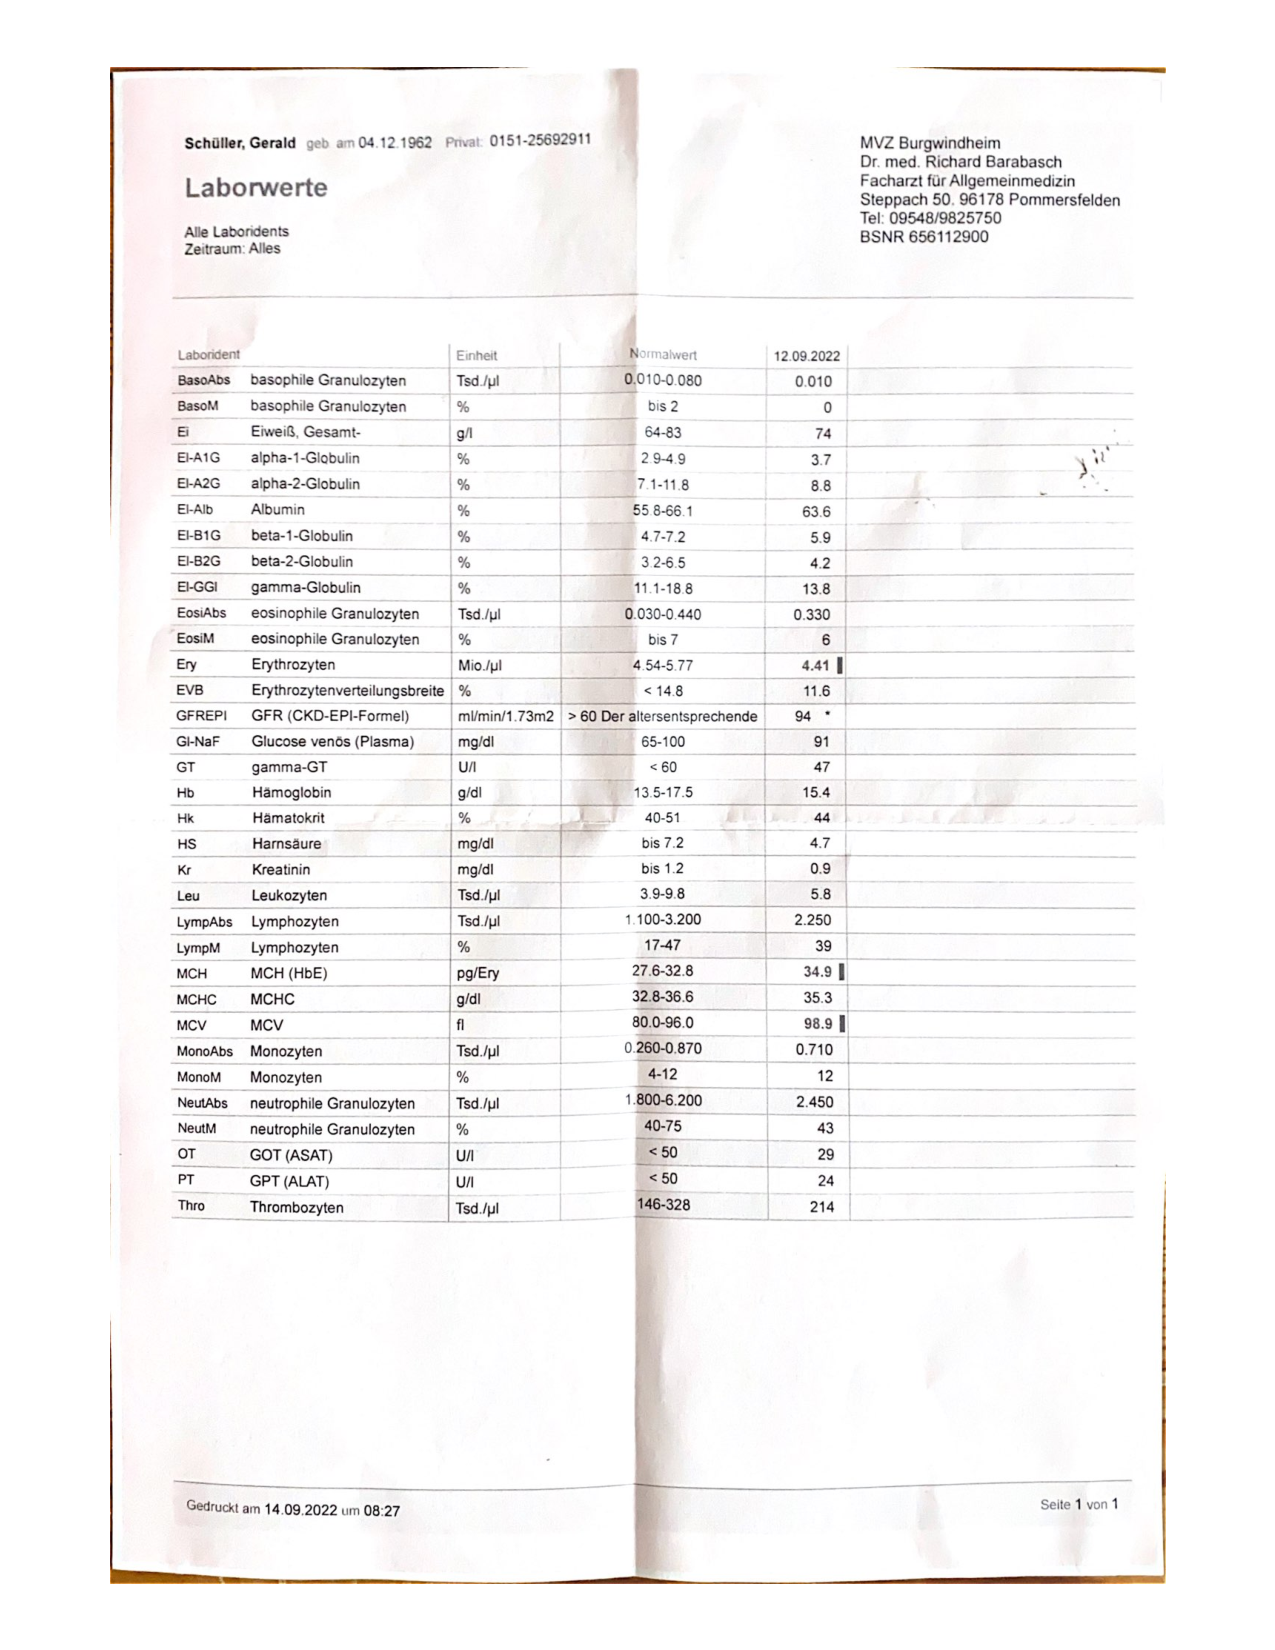
\includepdf[pages=-, scale=0.9, offset=0 0, pagecommand={%
    \begin{flushleft}  
        \section{Appendix}
      \end{flushleft} 
    \subsection{Laborwerte - 12.09.2022}\thispagestyle{plain}}
]{lw220912.pdf}

% Include the next pdf file.
% 
\includepdf[pages=-, scale=0.9, offset=0 0, pagecommand={%
%    \subsection{Ludwig Wittgenstein, Tractatus}\thispagestyle{plain}}
% ]{tractatus.pdf}


\subsection{Saaletalklinik}

\verb+https://saaletal.campus-nes.de/behandlungsangebot/unsere-kliniken/saaletalklinik.html+


\subsubsection{Therapiekonzept}

\verb+https://saaletal.campus-nes.de/fileadmin/user_upload/Therapiekonzept_Saaletalklinik_2014.pdf+


\subsubsection{Sportgeräte}

Liegestützgriffe \\
Roller 

\subsubsection{Zazen}

Sitzkissen \\
Matte


\subsection{Menübilder}

\verb+cd menue; mogrify -format png vleber.jpeg+ \\
\verb+cd menue; mogrify -format png eleber.jpeg+ \\
\verb+cd menu; gthumb vleber.png+

\vskip 4pt
\verb+https://tex.stackexchange.com/questions/234441/latex-includegraphics-width-and-height+


\subsubsection{Thunfisch mit Spinat-Ravioli}

\begin{figure}[H] % <-- Use [H] for exactly here
  
% \centering
\parbox{4cm}{
  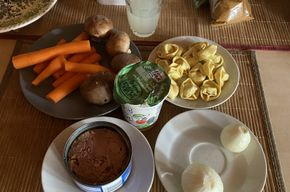
\includegraphics[
    width=4cm,
    height=3cm,
    keepaspectratio,
  ]{menue/vThunfischR.png}
\caption{Vorbereitung}}
\qquad
\begin{minipage}{4cm}
  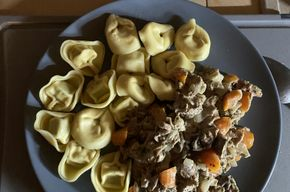
\includegraphics[
    width=4cm,
    height=3cm,
    keepaspectratio,
  ]{menue/eThunfischR.png}
\caption{Ergebnis}

\end{minipage}
\end{figure}


\subsubsection{Leber mit Bohnen}

\begin{figure}[H] % <-- Use [H] for exactly here
  
% \centering
\parbox{4cm}{
  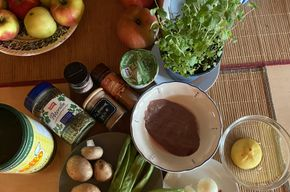
\includegraphics[
    width=4cm,
    height=3cm,
    keepaspectratio,
  ]{menue/vLeberBohnen.png}
\caption{Vorbereitung}}
\qquad
\begin{minipage}{4cm}
  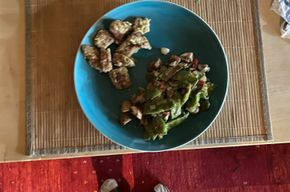
\includegraphics[
    width=4cm,
    height=3cm,
    keepaspectratio,
  ]{menue/eLeberBohnen.png}
\caption{Ergebnis}

\end{minipage}
\end{figure}


\subsubsection{Tofu mit Kartoffeln}

\begin{figure}[H] % <-- Use [H] for exactly here
  
% \centering
\parbox{4cm}{
  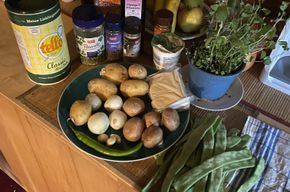
\includegraphics[
    width=4cm,
    height=3cm,
    keepaspectratio,
  ]{menue/vTofuKartoffeln.png}
\caption{Vorbereitung}}
\qquad
\begin{minipage}{4cm}
  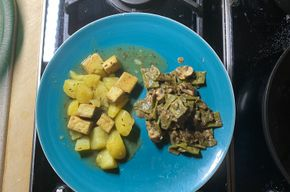
\includegraphics[
    width=4cm,
    height=3cm,
    keepaspectratio,
  ]{menue/eTofuKartoffeln.png}
\caption{Ergebnis}

\end{minipage}
\end{figure}


\subsubsection{Leber mit Kohlrabi}

\begin{figure}[H] % <-- Use [H] for exactly here
  
% \centering
\parbox{4cm}{
  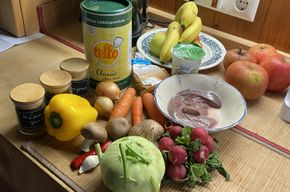
\includegraphics[
    width=4cm,
    height=3cm,
    keepaspectratio,
  ]{menue/vLeberKohlrabi.png}
\caption{Vorbereitung}}
\qquad
\begin{minipage}{4cm}
  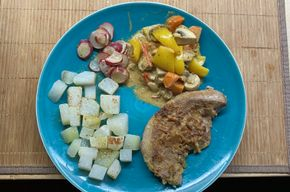
\includegraphics[
    width=4cm,
    height=3cm,
    keepaspectratio,
  ]{menue/eLeberKohlrabi.png}
\caption{Ergebnis}

\end{minipage}
\end{figure}


\subsubsection{Wiener mit Sauerkraut}

\begin{figure}[H] % <-- Use [H] for exactly here
  
% \centering
\parbox{4cm}{
  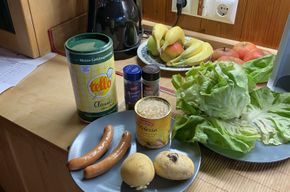
\includegraphics[
    width=4cm,
    height=3cm,
    keepaspectratio,
  ]{menue/vWienerSk.png}
\caption{Vorbereitung}}
\qquad
\begin{minipage}{4cm}
  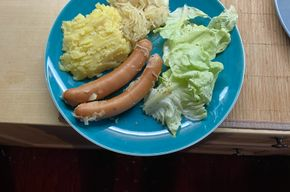
\includegraphics[
    width=4cm,
    height=3cm,
    keepaspectratio,
  ]{menue/eWienerSk.png}
\caption{Ergebnis}

\end{minipage}
\end{figure}


\subsubsection{Thunfisch mit Mohrrüben}

\begin{figure}[H] % <-- Use [H] for exactly here
  
% \centering
\parbox{4cm}{
  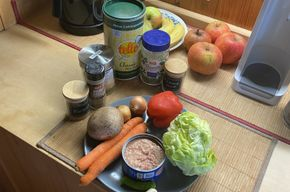
\includegraphics[
    width=4cm,
    height=3cm,
    keepaspectratio,
  ]{menue/vThunfischMr.png}
\caption{Vorbereitung}}
\qquad
\begin{minipage}{4cm}
  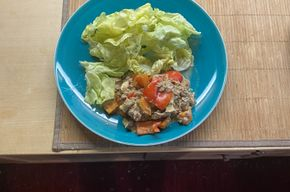
\includegraphics[
    width=4cm,
    height=3cm,
    keepaspectratio,
  ]{menue/eThunfischMr.png}
\caption{Ergebnis}

\end{minipage}
\end{figure}


\subsection{Charaktereigenschaften}

\verb+https://wortwuchs.net/charaktereigenschaften/+

abenteuerlustig \\
abergläubisch \\
abwesend \\
aggressiv \\
aktiv \\
analytisch \\
angriffslustig \\
ängstlich \\
anspruchsvoll \\
anstrengend \\
antriebslos \\
aufdringlich \\
aufgeregt \\
aufgeweckt \\
auflehnend \\
aufmerksam \\
ausdauernd \\
ausweichend \\
begeistert \\
begierig \\
begriffsstutzig \\
belastbar \\
bequem \\
besserwisserisch \\
beweglich \\
bissig \\
differenziert \\
dünnhäutig \\
durchtrieben \\
effizient \\
ehrgeizig \\
eingeschüchtert \\
einsam \\
einzelgängerisch \\
elitär \\
empfindlich \\
entscheidungsfreudig \\
entschlossen \\
ernst \\
exakt \\
fatalistisch \\
fleißig \\
flexibel \\
fokussierend \\
frech \\
freundlich
gedankenverloren \\
geduldig \\
gehemmt \\
gierig \\
größenwahnsinnig \\
grüblerisch \\
gründlich \\
harmlos \\
hinterfotzig \\
höflich \\
innovativ \\
instinktiv \\
interessiert \\
intuitiv \\
ironisch \\
jähzornig \\
kämpferisch \\
kalkulierend \\
klug \\
kompliziert \\
konsequent \\
konstruktiv \\
konzentriert \\
leichtsinnig \\
leistungsbereit \\
lernwillig \\
lethargisch \\
lösungsorientiert \\
menschenscheu \\
methodisch \\
mimosenhaft \\
misstrauisch \\
motiviert \\
mutig \\
nachdenklich \\
naiv \\
nervös \\
neugierig \\
niedergeschlagen \\
optimistisch \\
pingelig \\
pragmatisch \\
raffiniert \\
realistisch \\
reflektierend \\
religiös \\
schreckhaft \\
selbständig \\
schüchtern \\
selbstreflektierend \\
selbstüberschätzend \\
skeptisch \\
sorgfältig \\
spirituell \\
sportlich \\
sprunghaft \\
steif \\
still \\
stolz \\
strukturiert \\
tagträumerisch \\
träumerisch \\
überempfindlich \\
unsicher \\
verklemmt \\
verlässlich \\
verunsichert \\
verträumt \\
verwahrlost \\
wankelmütig \\
willensstark \\
wortkarg \\
zäh \\
zielorientiert \\
zuverlässig


% xxx
% Start of the library.
%

% Print the complete library.
\nocite{*}

\printbibheading


\printbibliography[keyword=Bilder, heading=subbibliography,
  title={Bilderbücher}]


\printbibliography[keyword=Vorschule, heading=subbibliography,
  title={Vorschule}]


\printbibliography[keyword=Schule, heading=subbibliography,
  title={Schulbücher}]


\printbibliography[keyword=Evolution, heading=subbibliography,
  title={Evolution}]


\subsection{Tractatus}

\verb+https://www.mathebibel.de/funktionen+ \\
\verb+https://home.mathematik.uni-freiburg.de/wolke/Schuster_Skript.pdf+ \\
\verb+http://www.fb10.uni-bremen.de/khwagner/grundkurs2/kapitel3.aspx+ \\
\verb+https://ftp.agdsn.de/pub/mirrors/latex/dante/fonts/stix/doc/stix.pdf+


\subsection{Märchen}

\subsubsection{Das Hirtenbüblein}

\verb+https://de.wikisource.org/wiki/Das_Hirtenb%C3%BCblein_(1857)+

\vskip 4pt
Es war einmal ein Hirtenbübchen, das war wegen seiner weisen Antworten, die es
auf alle Fragen gab, weit und breit berühmt. Der König des Landes hörte auch
davon, glaubte es nicht und ließ das Bübchen kommen. Da sprach er zu ihm
,,kannst du mir auf drei Fragen, die ich dir vorlegen will, Antwort geben, so
will ich dich ansehen wie mein eigen Kind, und du sollst bei mir in meinem
königlichen Schloß wohnen.'' Sprach das Büblein ,,wie lauten die drei Fragen?''
Der König sagte ,,die erste lautet wie viel Tropfen Wasser sind in dem
Weltmeer?'' Das Hirtenbüblein antwortete ,,Herr König, laßt alle Flüsse auf der
Erde verstopfen, damit kein Tröpflein mehr daraus ins Meer lauft, das ich nicht
erst gezählt habe, so will ich euch sagen, wie viel Tropfen im Meere sind.''
Sprach der König ,,die andere Frage lautet wie viel Sterne stehen am Himmel?''
Das Hirtenbübchen sagte ,,gebt mir einen großen Bogen weiß Papier,'' und dann
machte es mit der Feder so viel feine Punkte darauf, daß sie kaum zu sehen und
fast gar nicht zu zählen waren und einem die Augen vergiengen, wenn man darauf
blickte. Darauf sprach es ,,so viel Sterne stehen am Himmel, als hier Punkte auf
dem Papier zählt sie nur.'' Aber niemand war dazu im Stand. Sprach der König
,,die dritte Frage lautet wie viel Secunden hat die Ewigkeit?'' Da sagte das
Hirtenbüblein ,,in Hinterpommern liegt der Demantberg, der hat eine Stunde [284]
in die Höhe, eine Stunde in die Breite und eine Stunde in die Tiefe; dahin kommt
alle hundert Jahr ein Vögelein und wetzt sein Schnäblein daran, und wenn der
ganze Berg abgewetzt ist, dann ist die erste Secunde von der Ewigkeit vorbei.''

\vskip 4pt
Sprach der König ,,du hast die drei Fragen aufgelöst wie ein Weiser und sollst
fortan bei mir in meinem königlichen Schlosse wohnen, und ich will dich ansehen
wie mein eigenes Kind.“

\subsubsection{Frau Holle}

\verb+https://de.wikisource.org/wiki/Frau_Holle_(1857)+

\vskip 4pt
Eine Wittwe hatte zwei Töchter, davon war die eine schön und fleißig, die andere
häßlich und faul. Sie hatte aber die häßliche und faule, weil sie ihre rechte
Tochter war, viel lieber, und die andere mußte alle Arbeit thun und der
Aschenputtel im Hause sein. Das arme Mädchen mußte sich täglich auf die große
Straße bei einem Brunnen setzen, und mußte so viel spinnen, daß ihm das Blut aus
den Fingern sprang. Nun trug es sich zu, daß die Spule einmal ganz blutig war,
da bückte es sich damit in den Brunnen und wollte sie abwaschen: sie sprang ihm
aber aus der Hand und fiel hinab. Es weinte, lief zur Stiefmutter und erzählte
ihr das Unglück. Sie schalt es aber so heftig und war so unbarmherzig, daß sie
sprach ,,hast du die Spule hinunterfallen lassen, so hol sie auch wieder herauf.''
Da gieng das Mädchen zu dem Brunnen zurück und wußte nicht was es anfangen
sollte: und in seiner Herzensangst sprang es in den Brunnen hinein, um die Spule
zu holen. Es verlor die Besinnung, und als es erwachte und wieder zu sich selber
kam, war es auf einer schönen Wiese wo die Sonne schien und viel tausend Blumen
standen. Auf dieser Wiese gieng es fort und kam zu einem Backofen, der war
voller Brot; das Brot aber rief ,,ach, zieh mich raus, zieh mich raus, sonst
verbrenn ich: ich bin schon längst ausgebacken.'' Da trat es herzu, und holte
mit dem Brotschieber alles nach einander heraus. Danach gieng es weiter und kam
zu einem Baum, der hieng voll Äpfel, und rief ihm zu ,,ach schüttel mich,
schüttel mich, wir Äpfel sind alle mit einander reif.'' Da schüttelte es den
Baum, daß die Äpfel fielen als regneten sie, und schüttelte bis keiner mehr oben
war; und als es alle in einen Haufen zusammengelegt hatte, gieng es wieder
weiter. Endlich kam es zu einem kleinen Haus, daraus guckte eine alte Frau,
weil sie aber so große Zähne hatte, ward ihm angst, und es wollte fortlaufen.
Die alte Frau aber rief ihm nach ,,was fürchtest du dich, liebes Kind? bleib bei
mir, wenn du alle Arbeit im Hause ordentlich thun willst, so soll dirs gut gehn.
Du mußt nur Acht geben daß du mein Bett gut machst und es fleißig aufschüttelst,
daß die Federn fliegen, dann schneit es in der Welt; ich bin die Frau Holle.''
Weil die Alte ihm so gut zusprach, so faßte sich das Mädchen ein Herz, willigte
ein und begab sich in ihren Dienst. Es besorgte auch alles nach ihrer
Zufriedenheit, und schüttelte ihr das Bett immer gewaltig auf daß die Federn wie
Schneeflocken umher flogen; dafür hatte es auch ein gut Leben bei ihr, kein
böses Wort, und alle Tage Gesottenes und Gebratenes. Nun war es eine Zeitlang
bei der Frau Holle, da ward es traurig und wußte anfangs selbst nicht was ihm
fehlte, endlich merkte es daß es Heimweh war; ob es ihm hier gleich viel
tausendmal besser gieng als zu Haus, so hatte es doch ein Verlangen dahin.
Endlich sagte es zu ihr ,,ich habe den Jammer nach Haus kriegt, und wenn es mir
auch noch so gut hier unten geht, so kann ich doch nicht länger bleiben, ich muß
wieder hinauf zu den Meinigen.'' Die Frau Holle sagte ,,es gefällt mir, daß du
wieder nach Haus verlangst, und weil du mir so treu gedient hast, so will ich
dich selbst wieder hinauf bringen.'' Sie nahm es darauf bei der Hand und führte
es vor ein großes Thor. Das Thor ward aufgethan, und wie das Mädchen gerade
darunter stand, fiel ein gewaltiger Goldregen, und alles Gold blieb an ihm
hängen, so daß es über und über davon bedeckt war. ,,Das sollst du haben, weil
du so fleißig gewesen bist'' sprach die Frau Holle und gab ihm auch die Spule
wieder, die ihm in den Brunnen gefallen war. Darauf ward das Thor verschlossen,
und das Mädchen befand sich oben auf der Welt, nicht weit von seiner Mutter
Haus: und als es in den Hof kam, saß der Hahn auf dem Brunnen und rief

\vskip 4pt
,,kikeriki, \\
unsere goldene Jungfrau ist wieder hie.''

\vskip 4pt
Da gieng es hinein zu seiner Mutter, und weil es so mit Gold bedeckt ankam, ward
es von ihr und der Schwester gut aufgenommen.

\vskip 4pt
Das Mädchen erzählte alles, was ihm begegnet war, und als die Mutter hörte wie
es zu dem großen Reichthum gekommen war, wollte sie der andern häßlichen und
faulen Tochter gerne dasselbe Glück verschaffen. Sie mußte sich an den Brunnen
setzen und spinnen; und damit ihre Spule blutig ward, stach sie sich in die
Finger und stieß sich die Hand in die Dornhecke. Dann warf sie die Spule in den
Brunnen und sprang selber hinein. Sie kam, wie die andere, auf die schöne Wiese
und gieng auf demselben Pfade weiter. Als sie zu dem Backofen gelangte, schrie
das Brot wieder ,,ach, zieh mich raus, zieh mich raus, sonst verbrenn ich, ich
bin schon längst ausgebacken.'' Die Faule aber antwortete ,,da hätt ich Lust
mich schmutzig zu machen,'' und gieng fort. Bald kam sie zu dem Apfelbaum, der
rief ,,ach, schüttel mich, schüttel mich, wir Äpfel sind alle mit einander reif.''
Sie antwortete aber ,,du kommst mir recht, es könnte mir einer auf den Kopf
fallen,'' und gieng damit weiter. Als sie vor der Frau Holle Haus kam, fürchtete
sie sich nicht, weil sie von ihren großen Zähnen schon gehört hatte, und
verdingte sich gleich zu ihr. Am ersten Tag that sie sich Gewalt an, war fleißig
und folgte der Frau Holle, wenn sie ihr etwas sagte, denn sie dachte an das
viele Gold, das sie ihr schenken würde; am zweiten Tag aber fieng sie schon an
zu faullenzen, am dritten noch mehr, da wollte sie Morgens gar nicht aufstehen.
Sie machte auch der Frau Holle das Bett nicht wie sichs gebührte, und schüttelte
es nicht, daß die Federn aufflogen. Das ward die Frau Holle bald müde und sagte
ihr den Dienst auf. Die Faule war das wohl zufrieden und meinte nun würde der
Goldregen kommen; die Frau Holle führte sie auch zu dem Thor, als sie aber
darunter stand, ward statt des Goldes ein großer Kessel voll Pech ausgeschüttet.
,,Das ist zur Belohnung deiner Dienste'' sagte die Frau Holle und schloß das
Thor zu. Da kam die Faule heim, aber sie war ganz mit Pech bedeckt, und der Hahn
auf dem Brunnen, als er sie sah, rief

\vskip 4pt
,,kikeriki, \\
unsere schmutzige Jungfrau ist wieder hie.''

\vskip 4pt
Das Pech aber blieb fest an ihr hängen und wollte, so lange sie lebte, nicht
abgehen.

\subsubsection{Der Arme und der Reiche}

\verb+https://de.wikisource.org/wiki/Der_Arme_und_der_Reiche_(1857)+

\vskip 4pt
Vor alten Zeiten, als der liebe Gott noch selber auf Erden unter den Menschen
wandelte, trug es sich zu, daß er eines Abends müde war und ihn die Nacht
überfiel, bevor er zu einer Herberge kommen konnte. Nun standen auf dem Weg vor
ihm zwei Häuser einander gegenüber, das eine groß und schön, das andere klein
und ärmlich anzusehen, und gehörte das große einem Reichen, das kleine einem
armen Manne. Da dachte unser Herr Gott ,,dem Reichen werde ich nicht
beschwerlich fallen: bei ihm will ich übernachten.'' Der Reiche, als er an seine
Thüre klopfen hörte, machte das Fenster auf und fragte den Fremdling was er
suche? Der Herr antwortete ,,ich bitte um ein Nachtlager.'' Der Reiche guckte
den Wandersmann von Haupt bis zu den Füßen an, und weil der liebe Gott schlichte
Kleider trug und nicht aussah wie einer, der viel Geld in der Tasche hat,
schüttelte er mit dem Kopf und sprach ,,ich kann euch nicht aufnehmen, meine
Kammern liegen voll Kräuter und Samen, und sollte ich einen jeden beherbergen,
der an meine Thüre klopft, so könnte ich selber den Bettelstab in die Hand
nehmen. Sucht euch anderswo ein Auskommen.'' Schlug damit sein Fenster zu und
ließ den lieben Gott stehen. Also kehrte ihm der liebe Gott den Rücken und gieng
hinüber zu dem kleinen Haus. Kaum hatte er angeklopft, so klinkte der Arme schon
sein Thürchen auf und bat den Wandersmann einzutreten. ,,Bleibt die Nacht über
bei mir,'' sagte er ,,es ist schon finster, und heute könnt ihr doch nicht weiter
kommen.'' Das gefiel dem lieben Gott und er trat zu ihm ein. Die Frau des Armen
reichte ihm die Hand, hieß ihn willkommen und sagte er möchte sichs bequem
machen und vorlieb nehmen, sie hätten nicht viel, aber was es wäre, gäben sie
von Herzen gerne. Dann setzte sie Kartoffeln ans Feuer, und derweil sie kochten,
melkte sie ihre Ziege, damit sie ein wenig Milch dazu hätten. Und als der Tisch
gedeckt war, setzte sich der liebe Gott nieder und aß mit ihnen, und schmeckte
ihm die schlechte Kost gut, denn es waren vergnügte Gesichter dabei. Nachdem sie
gegessen hatten, und Schlafenszeit war, rief die Frau heimlich ihren Mann und
sprach ,,hör, lieber Mann, wir wollen uns heute Nacht eine Streu machen, damit
der arme Wanderer sich in unser Bett legen und ausruhen kann: er ist den ganzen
Tag über gegangen, da wird einer müde.'' ,,Von Herzen gern,'' antwortete er,
,,ich wills ihm anbieten,'' gieng zu dem lieben Gott und bat ihn, wenns ihm
recht wäre, möcht er sich in ihr Bett legen und seine Glieder ordentlich
ausruhen. Der liebe Gott wollte den beiden Alten ihr Lager nicht nehmen, aber
sie ließen nicht ab, bis er es endlich that und sich in ihr Bett legte: sich
selbst aber machten sie eine Streu auf die Erde. Am andern Morgen standen sie
vor Tag schon auf und kochten dem Gast ein Frühstück, so gut sie es hatten. Als
nun die Sonne durchs Fensterlein schien und der liebe Gott aufgestanden war, aß
er wieder mit ihnen und wollte dann seines Weges ziehen. Als er in der Thüre
stand, kehrte er sich um und sprach ,,weil ihr so mitleidig und fromm seid, so
wünscht euch dreierlei, das will ich euch erfüllen.'' Da sagte der Arme ,,was
soll ich mir sonst wünschen als die ewige Seligkeit, und daß wir zwei, so lang
wir leben, gesund dabei bleiben und unser nothdürftiges tägliches Brot haben;
fürs dritte weiß ich mir nichts zu wünschen.'' Der liebe Gott sprach ,,willst
du dir nicht ein neues Haus für das alte wünschen?'' ,,O ja,'' sagte der Mann,
,,wenn ich das auch noch erhalten kann, so wär mirs wohl lieb.'' Da erfüllte der
Herr ihre Wünsche, verwandelte ihr altes Haus in ein neues, gab ihnen nochmals
seinen Segen und zog weiter.

\vskip 4pt
Es war schon voller Tag, als der Reiche aufstand. Er legte sich ins Fenster und
sah gegenüber ein neues, reinliches Haus mit rothen Ziegeln, wo sonst eine alte
Hütte gestanden hatte. Da machte er große Augen, rief seine Frau herbei und
sprach ,,sag mir, was ist geschehen? Gestern Abend stand noch die alte elende
Hütte, und heute steht da ein schönes neues Haus. Lauf hinüber und höre wie das
gekommen ist.'' Die Frau gieng und fragte den Armen aus: er erzählte ihr
,,gestern Abend kam ein Wanderer, der suchte Nachtherberge, und heute Morgen
beim Abschied hat er uns drei Wünsche gewährt, die ewige Seligkeit, Gesundheit
in diesem Leben und das nothdürftige tägliche Brot dazu und zuletzt noch statt
unserer alten Hütte ein schönes neues Haus'' Die Frau des Reichen lief eilig
zurück und erzählte ihrem Manne wie alles gekommen war. Der Mann sprach ,,ich
möchte mich zerreißen und zerschlagen: hätt ich das nur gewußt! der Fremde ist
zuvor hier gewesen und hat bei uns übernachten wollen, ich habe ihn aber
abgewiesen.'' ,,Eil dich,'' sprach die Frau, ,,und setze dich auf dein Pferd,
so kannst du den Mann noch einholen, und dann mußt du dir auch drei Wünsche
gewähren lassen.''

\vskip 4pt
Der Reiche befolgte den guten Rath, jagte mit seinem Pferd davon und holte den
lieben Gott noch ein. Er redete fein und lieblich und bat er möchts nicht übel
nehmen, daß er nicht gleich wäre eingelassen worden, er hätte den Schlüssel zur
Hausthüre gesucht, derweil wäre er weggegangen: wenn er des Weges zurück käme,
müßte er bei ihm einkehren. ,,Ja,'' sprach der liebe Gott, ,,wenn ich einmal
zurückkomme, will ich es thun.'' Da fragte der Reiche ob er nicht auch drei
Wünsche thun dürfte, wie sein Nachbar? Ja, sagte der liebe Gott, das dürfte er
wohl, es wäre aber nicht gut für ihn, und er sollte sich lieber nichts
wünschen. Der Reiche meinte er wollte sich schon etwas aussuchen, das zu seinem
Glück gereiche, wenn er nur wüßte, daß es erfüllt würde. Sprach der liebe Gott
,,reit heim, und drei Wünsche, die du thust, die sollen in Erfüllung gehen.''

\vskip 4pt
Nun hatte der Reiche was er verlangte, ritt heimwärts und fieng an nachzusinnen
was er sich wünschen sollte. Wie er sich so bedachte und die Zügel fallen ließ,
fieng das Pferd an zu springen, so daß er immerfort in seinen Gedanken gestört
wurde und sie gar nicht zusammen bringen konnte. Er klopfte ihm an den Hals und
sagte ,,sei ruhig, Liese,'' aber das Pferd machte aufs neue Männerchen. Da ward
er zuletzt ärgerlich und rief ganz ungeduldig ,,so wollt ich, daß du den Hals
zerbrächst!'' Wie er das Wort ausgesprochen hatte, plump, fiel er auf die Erde,
und lag das Pferd todt und regte sich nicht mehr; damit war der erste Wunsch
erfüllt. Weil er aber von Natur geizig war, wollte er das Sattelzeug nicht im
Stich lassen, schnitts ab, hiengs auf seinen Rücken, und mußte nun zu Fuß gehen.
,,Du hast noch zwei Wünsche übrig'' dachte er und tröstete sich damit. Wie er
nun langsam durch den Sand dahin gieng, und zu Mittag die Sonne heiß brannte,
wards ihm so warm und verdrießlich zu Muth: der Sattel drückte ihn auf den
Rücken, auch war ihm noch immer nicht eingefallen, was er sich wünschen sollte.
,,Wenn ich mir auch alle Reiche und Schätze der Welt wünsche,'' sprach er zu
sich selbst, ,,so fällt mir hernach noch allerlei ein, dieses und jenes, das
weiß ich im voraus: ich wills aber so einrichten, daß mir gar nichts mehr übrig
zu wünschen bleibt.'' Dann seufzte er und sprach ,,ja, wenn ich der bairische
Bauer wäre, der auch drei Wünsche frei hatte, der wußte sich zu helfen, der
wünschte sich zuerst recht viel Bier, und zweitens so viel Bier als er trinken
könnte, und drittens noch ein Faß Bier dazu.'' Manchmal meinte er jetzt hätte
er es gefunden, aber hernach schiens ihm doch zu wenig. Da kam ihm so in die
Gedanken was es seine Frau jetzt gut hätte, die säße daheim in einer kühlen
Stube und ließe sichs wohl schmecken. Das ärgerte ihn ordentlich, und ohne daß
ers wußte, sprach er so hin ,,ich wollte die säße daheim auf dem Sattel, und
könnte nicht herunter, statt daß ich ihn da auf meinem Rücken schleppe.'' Und
wie das letzte Wort aus seinem Munde kam, so war der Sattel von seinem Rücken
verschwunden, und er merkte daß sein zweiter Wunsch auch in Erfüllung gegangen
war. Da ward ihm erst recht heiß, er fieng an zu laufen und wollte sich daheim
ganz einsam in seine Kammer hinsetzen und auf etwas Großes für den letzten
Wunsch sinnen. Wie er aber ankommt und die Stubenthür aufmacht, sitzt da seine
Frau mittendrin auf dem Sattel und kann nicht herunter, jammert und schreit. Da
sprach er ,,gib dich zufrieden, ich will dir alle Reichthümer der Welt herbei
wünschen, nur bleib da sitzen.'' Sie schalt ihn aber einen Schafskopf und sprach
,,was helfen mir alle Reichthümer der Welt, wenn ich auf dem Sattel sitze; du
hast mich darauf gewünscht, du mußt mir auch wieder herunter helfen.'' Er mochte
wollen oder nicht, er mußte den dritten Wunsch thun, daß sie vom Sattel ledig
wäre und herunter steigen könnte; und der Wunsch ward alsbald erfüllt. Also
hatte er nichts davon als Ärger, Mühe, Scheltworte und ein verlornes Pferd: die
Armen aber lebten vergnügt, still und fromm bis an ihr seliges Ende.

\subsubsection{Rumpelstilzchen}

\verb+https://de.wikisource.org/wiki/Rumpelstilzchen_(1857)+

\vskip 4pt
Es war einmal ein Müller, der war arm, aber er hatte eine schöne Tochter. Nun
traf es sich, daß er mit dem König zu sprechen kam, und um sich ein Ansehen zu
geben, sagte er zu ihm ,,ich habe eine Tochter, die kann Stroh zu Gold spinnen.''
Der König sprach zum Müller ,,das ist eine Kunst, die mir wohl gefällt, wenn
deine Tochter so geschickt ist, wie du sagst, so bring sie Morgen in mein
Schloß, da will ich sie auf die Probe stellen.'' Als nun das Mädchen zu ihm
gebracht ward, führte er es in eine Kammer, die ganz voll Stroh lag, gab ihr Rad
und Haspel und sprach ,,jetzt mache dich an die Arbeit, und wenn du diese Nacht
durch bis morgen früh dieses Stroh nicht zu Gold versponnen hast, so mußt du
sterben.'' Darauf schloß er die Kammer selbst zu, und sie blieb allein darin.

\vskip 4pt
Da saß nun die arme Müllerstochter und wußte um ihr Leben keinen Rath: sie
verstand gar nichts davon, wie man Stroh zu Gold spinnen konnte, und ihre Angst
ward immer größer, daß sie endlich zu weinen anfieng. Da gieng auf einmal die
Thüre auf, und trat ein kleines Männchen herein und sprach ,,guten Abend,
Jungfer Müllerin, warum weint sie so sehr?'' ,,Ach,'' antwortete das Mädchen,
,,ich soll Stroh zu Gold spinnen, und verstehe das nicht.'' Sprach das Männchen
,,was gibst du mir, wenn ich dirs spinne?'' ,,Mein Halsband'' sagte das Mädchen.
Das Männchen nahm das Halsband, setzte sich vor das Rädchen, und schnurr,
schnurr, schnurr, dreimal gezogen, war die Spule voll. Dann steckte es eine
andere auf, und schnurr, schnurr, schnurr, dreimal gezogen, war auch die zweite
voll: und so giengs fort bis zum Morgen, da war alles Stroh versponnen, und alle
Spulen waren voll Gold. Bei Sonnenaufgang kam schon der König und als er das
Gold erblickte, erstaunte er und freute sich, aber sein Herz ward nur noch
goldgieriger. Er ließ die Müllerstochter in eine andere Kammer voll Stroh
bringen, die noch viel größer war, und befahl ihr das auch in einer Nacht zu
spinnen, wenn ihr das Leben lieb wäre. Das Mädchen wußte sich nicht zu helfen
und weinte, da gieng abermals die Thüre auf, und das kleine Männchen erschien
und sprach ,,was gibst du mir, wenn ich dir das Stroh zu Gold spinne?'' ,,Meinen
Ring von dem Finger'' antwortete das Mädchen. Das Männchen nahm den Ring, fieng
wieder an zu schnurren mit dem Rade und hatte bis zum Morgen alles Stroh zu
glänzendem Gold gesponnen. Der König freute sich über die Maßen bei dem Anblick,
war aber noch immer nicht Goldes satt, sondern ließ die Müllerstochter in eine
noch größere Kammer voll Stroh bringen und sprach ,,die mußt du noch in dieser
Nacht verspinnen: gelingt dirs aber, so sollst du meine Gemahlin werden.''
,,Wenns auch eine Müllerstochter ist,'' dachte er, ,,eine reichere Frau finde
ich in der ganzen Welt nicht.'' Als das Mädchen allein war, kam das Männlein
zum drittenmal wieder und sprach ,,was gibst du mir, wenn ich dir noch diesmal
das Stroh spinne?'' ,,Ich habe nichts mehr, das ich geben könnte'' antwortete
das Mädchen. ,,So versprich mir, wenn du Königin wirst, dein erstes Kind.''
,,Wer weiß wie das noch geht'' dachte die Müllerstochter und wußte sich auch in
der Noth nicht anders zu helfen; sie versprach also dem Männchen was es
verlangte, und das Männchen spann dafür noch einmal das Stroh zu Gold. Und als
am Morgen der König kam und alles fand wie er gewünscht hatte, so hielt er
Hochzeit mit ihr, und die schöne Müllerstochter ward eine Königin.

\vskip 4pt
Über ein Jahr brachte sie ein schönes Kind zur Welt und dachte gar nicht mehr an
das Männchen: da trat es plötzlich in ihre Kammer und sprach ,,nun gib mir was
du versprochen hast.'' Die Königin erschrack und bot dem Männchen alle
Reichthümer des Königreichs an, wenn es ihr das Kind lassen wollte: aber das
Männchen sprach ,,nein, etwas lebendes ist mir lieber als alle Schätze der Welt.''
Da fieng die Königin so an zu jammern und zu weinen, daß das Männchen Mitleiden
mit ihr hatte: ,,drei Tage will ich dir Zeit lassen,'' sprach er, ,,wenn du bis
dahin meinen Namen weißt, so sollst du dein Kind behalten.''

\vskip 4pt
Nun besann sich die Königin die ganze Nacht über auf alle Namen, die sie jemals
gehört hatte, und schickte einen Boten über Land, der sollte sich erkundigen
weit und breit was es sonst noch für Namen gäbe. Als am andern Tag das Männchen
kam, fieng sie an mit Caspar, Melchior, Balzer, und sagte alle Namen, die sie
wußte, nach der Reihe her, aber bei jedem sprach das Männlein ,,so heiß ich
nicht.'' Den zweiten Tag ließ sie in der Nachbarschaft herumfragen wie die Leute
da genannt würden, und sagte dem Männlein die ungewöhnlichsten und seltsamsten
Namen vor, ,,heißt du vielleicht Rippenbiest oder Hammelswade oder Schnürbein?''
aber es antwortete immer ,,so heiß ich nicht.'' Den dritten Tag kam der Bote
wieder zurück und erzählte ,,neue Namen habe ich keinen einzigen finden können,
aber wie ich an einen hohen Berg um die Waldecke kam, wo Fuchs und Has sich gute
Nacht sagen, so sah ich da ein kleines Haus, und vor dem Haus brannte ein Feuer,
und um das Feuer sprang ein gar zu lächerliches Männchen, hüpfte auf einem Bein
und schrie

\vskip 4pt
,,heute back ich, morgen brau ich, \\
übermorgen hol ich der Königin ihr Kind; \\
ach, wie gut ist daß niemand weiß \\
daß ich Rumpelstilzchen heiß!''

\vskip 4pt
Da könnt ihr denken wie die Königin froh war, als sie den Namen hörte, und als
bald hernach das Männlein herein trat und fragte ,,nun, Frau Königin, wie heiß
ich?'' fragte sie erst ,,heißest du Kunz?'' ,,Nein.'' ,,Heißest du Heinz?''
,,Nein.''

\vskip 4pt
,,Heißt du etwa Rumpelstilzchen?''

\vskip 4pt
,,Das hat dir der Teufel gesagt, das hat dir der Teufel gesagt'' schrie das
Männlein und stieß mit dem rechten Fuß vor Zorn so tief in die Erde, daß es bis
an den Leib hineinfuhr, dann packte es in seiner Wuth den linken Fuß mit beiden
Händen und riß sich selbst mitten entzwei.


\subsection{Zensus}

\subsubsection{Bibliographie}

\verb+https://www.zensus2022.de/DE/Was-ist-der-Zensus/_inhalt.html+

\subsubsection{Definitionen}

\begin{mdframed}[style=daystyle, leftmargin=-25pt]
  \begin{itemize}
    \setlength\itemsep{-3pt}
  \item {\emps {Zensus}} 2022 findet in Deutschland wieder ein Zensus statt. Mit
    dieser statistischen Erhebung wird ermittelt, wie viele Menschen in
    Deutschland leben, wie sie wohnen und arbeiten.
  \end{itemize}
\end{mdframed}

\subsubsection{Anmeldung}

\begin{labeling}{Anzahl der Wohnungen:}
  \setlength\itemsep{-3pt}
\item[Zugangsnummer:]        4032 7571 6347
\item[Atkivierungscode:]     5u9j99mh6wg
\item[Anschrift:]            Ich bin Eigentümer
\item[Gebäude:]              Wohngebäude 
\item[Anzahl der Wohnungen:] 1
\item[Fertigstellung:]       2011
\item[Gebäudetyp:]           Freistehendes Einfamilienhaus
\item[Eigentümer:]           Privatpersion
\item[Heizungsart:]          Zentralheizung
\item[Energieträger:]        Holz
\item[Wohnungsnutzung:]      Vom Eigentümer bewohnt
\item[Anzahl der Personen:]  2
\item[Namen:]                Schüller Gerald, Schleicher Renate
\item[Wohnfläche:]           128 $m^2$
\item[Anzahl der Räume:]     6
\item[Weitere Wohngebäude:]  Nein
\end{labeling}

\subsection{Grundsteuer}

\subsubsection{Bibliographie}

\verb+https://de.wikipedia.org/wiki/Grundsteuer+ \\
\verb+https://www.bundesfinanzministerium.de/Content/DE/FAQ/faq-die-neue-grundsteuer.html+ \\
\verb+https://www.elster.de/eportal/start+

\subsubsection{Definitionen}

\begin{mdframed}[style=daystyle, leftmargin=-25pt]
  \begin{itemize}
    \setlength\itemsep{-3pt}
  \item {\emps {Grundsteuer}} (Bodenzins) ist eine Geldleistung für ein
    Eigentum an einem Teil der Erdoberfläche, das im Grundbuch beschrieben wird.
  \end{itemize}
\end{mdframed}

\subsubsection{Grundsteuererklärung}

\begin{enumerate}[label={\Square}]
    \setlength\itemsep{-3pt}
  
  \item [\XBox] Das Dokument muss ich bis zum 31.10.2022 abgeben.
    
  \item [\XBox] Die Erklärung muss ich elektronisch über das ELSTER-Portal an das
    Finanzamt übermitteln.
    
  \item [\XBox] Ein ELSTER-Zertifikat erhalte ich unter \verb+https://www.elster.de/eportal/start+
    
  \item [\XBox] Für das ELSTER-Login benötige ich eine Zertifikationsdatei und ein Passwort.
    
  \item [\XBox] Zugang bekomme ich mit der steuerlichen Identifikationsnummer: \\
    IdNr.: 62 098 453 150; Benutzername: hozan; Lieblingsbuch: Tractatus
    
  \item [\XBox] Ich erhalte zwei Briefe: Aktivierungs-Code und Abrufcode.
    
  \item [\XBox] Per EMail bestätige ich die Aktivierung meines Benutzerkontos: \\
    Benutzername: hozan; Aktivierungs-ID: 282875961012266960
    
  \item [\XBox] Innerhalb von 14 Tagen schickt mir das Finanzamt den Aktivierungs-Code
    postalisch.
    
  \item [\XBox] Mit dem Aktivierungs-Code kann ich die Registrierung fortsetzen: \\
    Aktivierungs-ID: 282875961012266960 \\
    Aktivierungs-Code: 9UZL-AMTL-M4HJ
    
  \item [\XBox] Zertifikationsdatei erstellen: \\
    Name der Zertifikatsdatei: hozan\_elster\_29.09.2022\_14.32.pfx \\
    Passwort für Login: =Logisch2022

  \item [\XBox] Zertifikatsdatei herunterladen: ~/Download/hozan\_elster\_29.09.2022\_14.32.pfx

  \item [\XBox] Erstmaliges Login - Mein Profil ergänzen: \\
    Steuernummer: 207/684/07526

  \item [\XBox] Benutzerkontoinformationen \\
      Gerald Josef Schüller \\
      Benutzerkonto-ID: 1091780273

      \vskip 4pt
      Registriert am \\
      29.09.2022

      \vskip 4pt
      Identifiziert mit \\
      Identifikationsnummer: 62098453150
      
      \vskip 4pt
      Art des Zertifikats \\
      Persönliches Zertifikat 

      \vskip 4pt
      Gültigkeit des Zertifikats \\
      Gültig bis: 29.09.2025 um 14:36 Uhr

    \item [\XBox] Mein ELSTER: Alle Formulare: Grundsteuer: Grundsteuer für Bayern

    \item Grundsteuer für Bayern \\
      Für das Ausfüllen des Formulars benötigen Sie je nach persönlicher
      Situation unter anderem folgende Informationen:

      \vskip 4pt
      Aktenzeichen Ihres Grundstücks bzw. Ihres Betriebs der Land- und Forstwirtschaft \\
      Flurstücksfläche \\
      Flurstücksnummer \\
      Gebäudefläche

      \vskip 4pt
      Weitere Informationen finden Sie unter www.grundsteuer.bayern.de.

      \vskip 4pt
      Vom 1. Juli 2022 bis zum 31. Dezember 2022 können Sie ausgewählte Daten,
      wie z. B. Flurstücksnummer und amtliche Fläche, aus dem
      Liegenschaftskataster zum Stichtag 1. Januar 2022 kostenlos über das
      Internetportal BayernAtlas-Grundsteuerabrufen. Beim BayernAtlas-Grundsteuer
      handelt es sich um ein Angebot der Bayerischen Vermessungsverwaltung. Sie
      können der Veröffentlichung der Daten zu Ihrem Flurstück im
      BayernAtlas-Grund\-steuer widersprechen:
      
      \vskip 4pt
      \verb+https://www.ldbv.bayern.de/produkte/grundsteuer.html+

\end{enumerate}

% \subsubsection{Aktenzeichen}

% Include the pdf file.
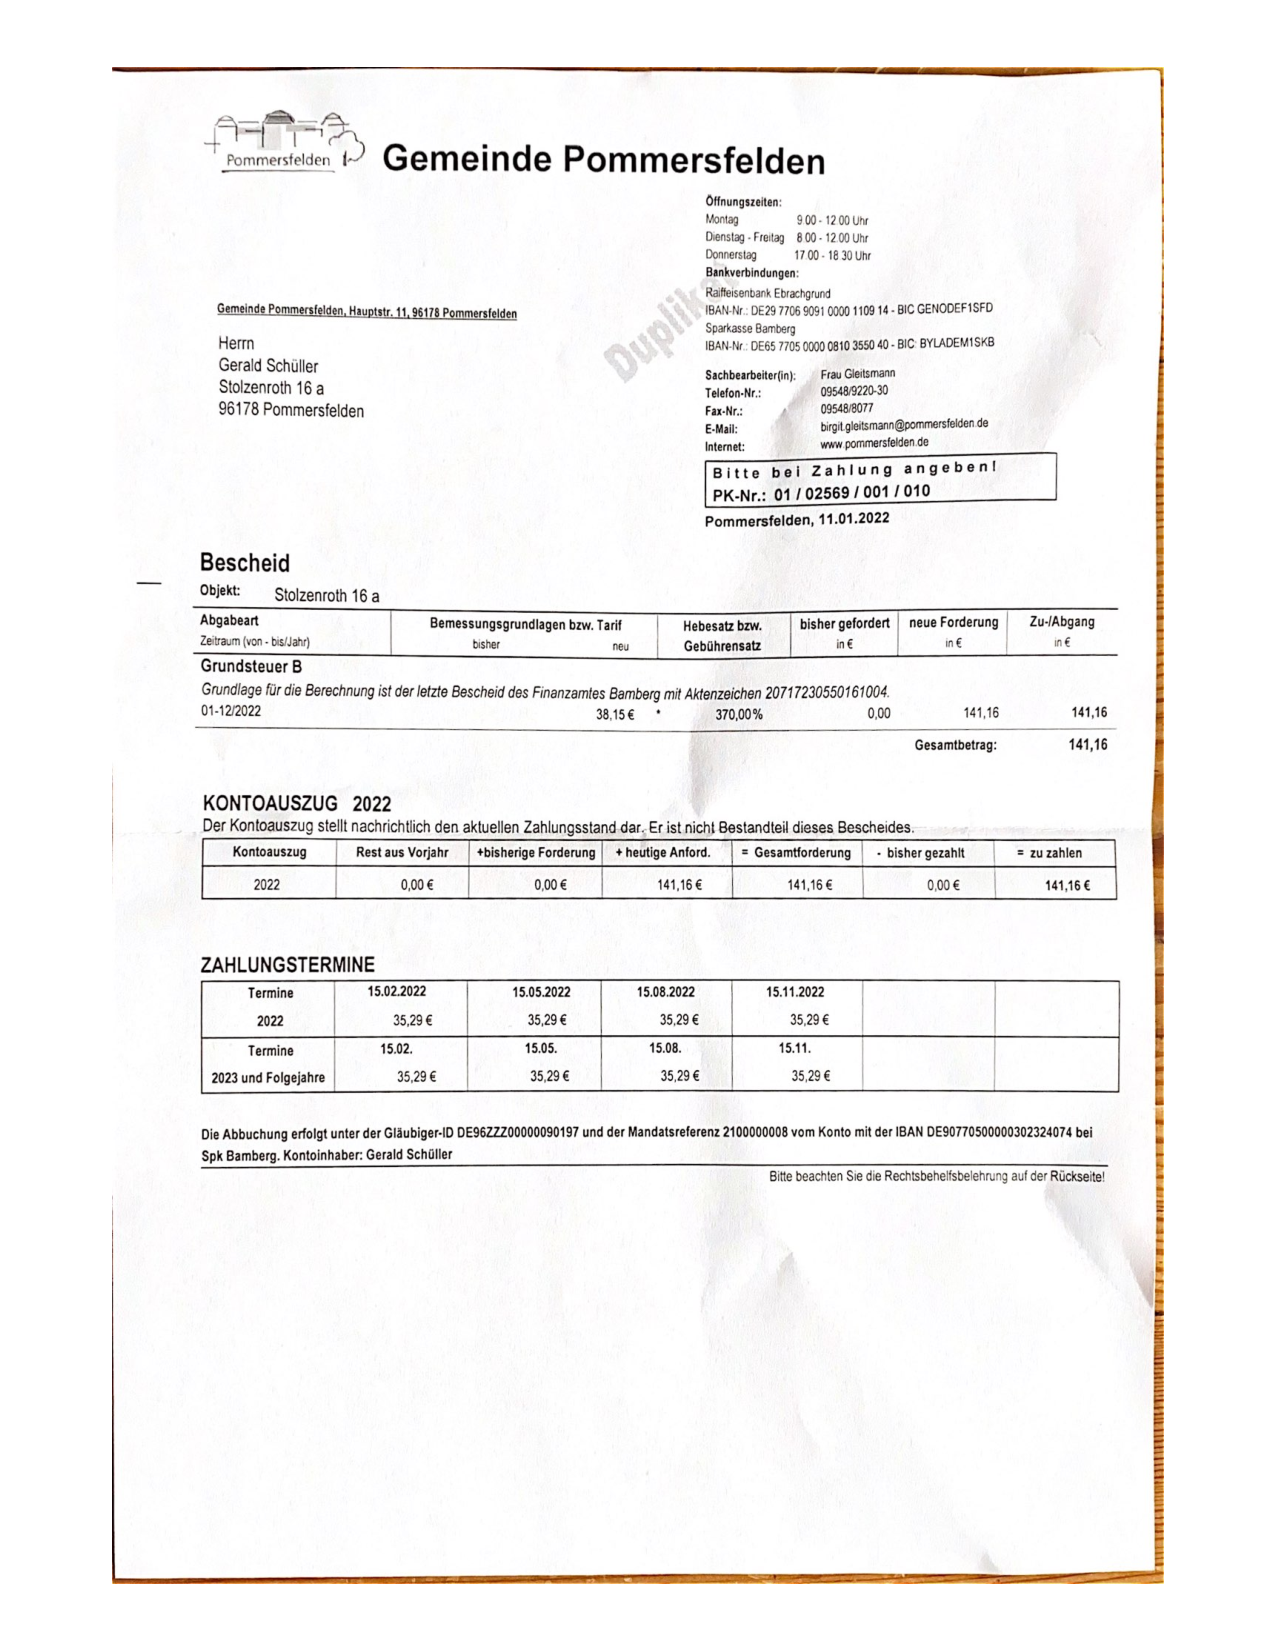
\includepdf[pages=-, scale=0.9, offset=0 0, pagecommand={%
    \begin{flushleft}  
        \subsubsection{Aktenzeichen}
      \end{flushleft} 
    \paragraph{Bescheid}\thispagestyle{plain}}
]{GrstAktz.pdf}


\subsection{Ausblick}

\subsubsection{Muskelaufbau}

\verb+https://www.welt.de/sport/fitness/plus214620124+ \\
\verb+/Fitness-Training-Die-groessten-Fehler-beim-Muskelaufbau.html+

% End of a LaTeX text, that is to be printed.

\end{document}
